%% Based on a TeXnicCenter-Template by Tino Weinkauf.
%%%%%%%%%%%%%%%%%%%%%%%%%%%%%%%%%%%%%%%%%%%%%%%%%%%%%%%%%%%%%

%%%%%%%%%%%%%%%%%%%%%%%%%%%%%%%%%%%%%%%%%%%%%%%%%%%%%%%%%%%%%
%% HEADER
%%%%%%%%%%%%%%%%%%%%%%%%%%%%%%%%%%%%%%%%%%%%%%%%%%%%%%%%%%%%%
\documentclass[a4paper,twoside,11pt]{article}
% Alternative Options:
%	Paper Size: a4paper / a5paper / b5paper / letterpaper / legalpaper / executivepaper
% Duplex: oneside / twoside
% Base Font Size: 10pt / 11pt / 12pt


%% Language %%%%%%%%%%%%%%%%%%%%%%%%%%%%%%%%%%%%%%%%%%%%%%%%%
\usepackage[USenglish]{babel} %francais, polish, spanish, ...
\usepackage[T1]{fontenc}
%%\usepackage[ansinew]{inputenc}

\usepackage{lmodern} %Type1-font for non-english texts and characters

%% NG: Try the following for sans serif.
%% Well - take your pick. helvet leaves math in serif. But is otherwise rather nice?
\usepackage[scaled]{helvet}
%%\usepackage[math]{kurier}  %% Not nice.
%%\usepackage[math]{iwona}   %% Not nice.
%%\usepackage{cmbright}      %% Still will not work after installing hfbright.
\renewcommand*\familydefault{\sfdefault}

\usepackage{eulervm}
\usepackage{url}

%% NG: Try this for colour.
\usepackage{color}

\usepackage{float}

%% NG: Try this for HTML output
%% Also choose LaTeX => HTML of course ...
%%\usepackage[html]{tex4ht}

%% Packages for Graphics & Figures %%%%%%%%%%%%%%%%%%%%%%%%%%
\usepackage{graphicx} %%For loading graphic files
%\usepackage{subfig} %%Subfigures inside a figure
%\usepackage{tikz} %%Generate vector graphics from within LaTeX

%% Please note:
%% Images can be included using \includegraphics{filename}
%% resp. using the dialog in the Insert menu.
%% 
%% The mode "LaTeX => PDF" allows the following formats:
%%   .jpg  .png  .pdf  .mps
%% 
%% The modes "LaTeX => DVI", "LaTeX => PS" und "LaTeX => PS => PDF"
%% allow the following formats:
%%   .eps  .ps  .bmp  .pict  .pntg

%% NG: Try this to scale graphics to be at most the line length wide.
%% \includegraphics[width=\maxwidth]{figure}
\makeatletter
\def\maxwidth{%
  \ifdim\Gin@nat@width>\linewidth
    \linewidth
  \else
    \Gin@nat@width
  \fi
}
\makeatother

%% NG: Try fancy chapter headings.
%% This is Ulf Lindgren's FncyChap package. But set to Sans.
%\usepackage[Lenny]{fncychap}
%\ChTitleVar{\Huge\bfseries\sf}
%\usepackage[Glenn]{fncychap}
%\ChTitleVar{\Large\bfseries\sf}

%% NG: And we might want text in a box.
\usepackage{boxedminipage}

%% Math Packages %%%%%%%%%%%%%%%%%%%%%%%%%%%%%%%%%%%%%%%%%%%%
\usepackage{amsmath}
\usepackage{amsthm}
\usepackage{amsfonts}
\usepackage{mathrsfs}


%% Line Spacing %%%%%%%%%%%%%%%%%%%%%%%%%%%%%%%%%%%%%%%%%%%%%
%\usepackage{setspace}
%\singlespacing        %% 1-spacing (default)
%\onehalfspacing       %% 1,5-spacing
%\doublespacing        %% 2-spacing


%% Other Packages %%%%%%%%%%%%%%%%%%%%%%%%%%%%%%%%%%%%%%%%%%%
\usepackage{a4wide} %%Smaller margins = more text per page.
\usepackage{fancyhdr} %%Fancy headings
%\usepackage{longtable} %%For tables, that exceed one page

%% NG: Fancy verbatim text
\usepackage{relsize,fancyvrb}

%% NG: Font for Creative Commons license thing
\usepackage{cclicenses}

%% NG: Try barcodes (crumbs!)
%\usepackage{pst-barcode,pstricks-add}

%% NG: Node diagrams
\usepackage{pstricks,pst-node}

%% NG: Landscape?
\usepackage{lscape}

%% NG: Source code listings
\usepackage{listings,color}
\lstloadlanguages{Python,bash}
\lstdefinestyle{cp}{
  language=Python,
  frame=single,
  showstringspaces=false,
  basicstyle=\footnotesize\ttfamily
}
\lstdefinestyle{sh}{
  language=bash,
  frame=single,
  showstringspaces=false,
  basicstyle=\footnotesize\ttfamily
}
\lstdefinestyle{cpt}{
  language=Python,
  frame=single,
  showstringspaces=false,
  basicstyle=\tiny\ttfamily
}
\lstset{style=sh}

%% Index
%\usepackage{makeidx}
%\makeindex


%%%%%%%%%%%%%%%%%%%%%%%%%%%%%%%%%%%%%%%%%%%%%%%%%%%%%%%%%%%%%
%% Remarks
%%%%%%%%%%%%%%%%%%%%%%%%%%%%%%%%%%%%%%%%%%%%%%%%%%%%%%%%%%%%%
%
% TODO:
% 1. Edit the used packages and their options (see above).
% 2. If you want, add a BibTeX-File to the project
%    (e.g., 'literature.bib').
% 3. Happy TeXing!
%
%%%%%%%%%%%%%%%%%%%%%%%%%%%%%%%%%%%%%%%%%%%%%%%%%%%%%%%%%%%%%

%%%%%%%%%%%%%%%%%%%%%%%%%%%%%%%%%%%%%%%%%%%%%%%%%%%%%%%%%%%%%
%% Options / Modifications
%%%%%%%%%%%%%%%%%%%%%%%%%%%%%%%%%%%%%%%%%%%%%%%%%%%%%%%%%%%%%

%\input{options} %You need a file 'options.tex' for this
%% ==> TeXnicCenter supplies some possible option files
%% ==> with its templates (File | New from Template...).
\newcommand{\newpara}{\par\vspace{4mm}\noindent}
\newcommand{\myldots}{\ldots\ }

\addto\captionsUSenglish{\renewcommand*\abstractname{Summary}}

% Let us try bold text in red ...
\definecolor{OurRed}{rgb}{0.9,0.1,0.1}
\newcommand{\textbfc}[1]{\textbf{\textcolor{OurRed}{#1}}}
\newcommand{\textttc}[1]{\texttt{\textcolor{OurRed}{#1}}}
\newcommand{\textc}[1]{\textcolor{OurRed}{#1}}

% And in green ...
\definecolor{OurGreen}{rgb}{0.1,0.5,0.1}
\newcommand{\textbfg}[1]{\textbf{\textcolor{OurGreen}{#1}}}

% Alter some LaTeX defaults for better treatment of figures:
    % See p.105 of "TeX Unbound" for suggested values.
    % See pp. 199-200 of Lamport's "LaTeX" book for details.
    %   General parameters, for ALL pages:
    \renewcommand{\topfraction}{0.9}	% max fraction of floats at top
    \renewcommand{\bottomfraction}{0.8}	% max fraction of floats at bottom
    %   Parameters for TEXT pages (not float pages):
    \setcounter{topnumber}{2}
    \setcounter{bottomnumber}{2}
    \setcounter{totalnumber}{4}     % 2 may work better
    \setcounter{dbltopnumber}{2}    % for 2-column pages
    \renewcommand{\dbltopfraction}{0.9}	% fit big float above 2-col. text
    \renewcommand{\textfraction}{0.07}	% allow minimal text w. figs
    %   Parameters for FLOAT pages (not text pages):
    \renewcommand{\floatpagefraction}{0.7}	% require fuller float pages
	% N.B.: floatpagefraction MUST be less than topfraction !!
    \renewcommand{\dblfloatpagefraction}{0.7}	% require fuller float pages

%% argmin math operator    
\DeclareMathOperator*{\argmin}{\arg\!\min}

%% Choose to include the giant COMP figures or NOT.
\newif\ifinclcomp
\inclcompfalse
%%\inclcomptrue

    
\usepackage[xetex,unicode,
	pdftitle={GPLOT: A DIMFILM Based Graph Plotting Program for CDC NOS 2.8},
	pdfauthor={Nick Glazzard},
	colorlinks,linkcolor=blue,citecolor=blue,urlcolor=blue
	]{hyperref}

%%%%%%%%%%%%%%%%%%%%%%%%%%%%%%%%%%%%%%%%%%%%%%%%%%%%%%%%%%%%%
%% DOCUMENT
%%%%%%%%%%%%%%%%%%%%%%%%%%%%%%%%%%%%%%%%%%%%%%%%%%%%%%%%%%%%%
\begin{document}

\title{\textbf{GPLOT}: A \textbf{DIMFILM} Based Graph Plotting Program \\ for CDC NOS 2.8}
\author{Nick Glazzard}
%%\date{November 20, 2012}
\maketitle


%%\begin{abstract}
%%Stuff
%%\end{abstract}

%%\clearpage

%%\tableofcontents

%%\clearpage

\section{Introduction}
\newpara
\textbf{GPLOT} is an interactive graphics program based on U.L.C.C. \textbf{DIMFILM}, a substantial graphics
library written and maintained
by Dr. John Gilbert between 1972 and approximately 1995. The version of \textbf{DIMFILM} used is
from somewhere around 1984 and is the second major version, which moved away from CDC Fortran
to portable, standard Fortran-77 (necessitated by U.L.C.C.'s move to Amdahl IBM compatible machines). 
\newpara
\textbf{GPLOT}, in contrast, was deliberately written for the CDC \texttt{FTN5} compiler under NOS 2.8 and
was not intended to be portable. It uses seven letter identifiers, dynamic memory allocation (via
the Common Memory Manager), and makes some use of NOS system calls.
\newpara
That said, it can be built and used on ``Unix-like'' systems (Debian Linux and macOS have been tested)
where it behaves almost identically to the NOS version.
\newpara
Originally, \textbf{GPLOT} was focussed on plotting graphs from tabulated data and could perhaps be thought of
as a stripped down \textbf{Gnuplot}, though with far fewer capabilities.
Recent versions have extended its capabilities in new directions so that it can be used for drawing block diagrams,
tables and other technical drawings.
\newpara
The primary `interactive' output device for \textbf{GPLOT} is \textbf{GTerm} -- a simple terminal emulator with colour graphics
capabilities written in Python (see the \textbf{GTerm} project repository for more information). \textbf{GPLOT} also 
supports Tektronix 401x terminals (which \texttt{xterm} emulates, although Ren\'{e} Richarz's
excellent 4014 emulator is preferred).
\newpara
Output in the form of graphics files which  can be included in other documents is available in two formats:
Encapsulated PostScript files and SVG files. The latter is 
used by the \textbf{PMDHTML} Markdown to HTML program and the \textbf{PLNOTES} short document maintenance scheme for NOS
(which is not described further here) as well as for HTML documents in general. The former is useful for \LaTeX and other
``print'' style document systems.
\newpara
A major goal for \textbf{GPLOT} is that it should be \textit{very easy to use} --- as easy as other graph plotting
programs on modern operating systems (such an \textbf{Gnuplot}, matplotlib, etc.) --- although \textbf{GPLOT} is not
directly comparable to those programs. In some aspects, it does much less than they do, but it also does
things they do not do.
\newpara
To build and install \textbf{GPLOT} on an emulated CYBER mainframe (with DtCyber), or on a ``Unix-like'' system,
please refer to the main \textbf{GPLOT} Github project \texttt{README.md}. This describes the build procedures in
a step-by-step fashion and also explains how a single source code base can be used fairly easily on both NOS and
``Unix-like'' systems.
\newpara
\textbf{GPLOT} (with \textbf{DIMFILM}) is almost entirely self-contained -- it has no dependencies beyond the operating
system and language runtime libraries. By modern standards, it is very light weight. It should be possible to
port it to other systems with working Fortran-77 compilers and runtimes, provided they do not insist on six character
variable and function names (although it would not be very hard to work around that with a simple Python program
to transform the source code). Many historic systems, as well as almost all modern systems, should be able to
build and run it. That said, it will almost certainly not run on systems as small as PDP-11s.


\section{Running \textbf{GPLOT}}
\textbf{GPLOT} needs two files: \texttt{GPLOT} (the pre-loaded binary executable) 
and \texttt{DADIMFO} (which contains
the font data for \textbf{DIMFILM}). To run \textbf{GPLOT} on NOS, use:
\begin{verbatim}
/ATTACH,GPLOT.
/GPLOT.
\end{verbatim}
\texttt{GPLOT} will \texttt{ATTACH} the font file (\texttt{DADIMFO}) itself.
On NOS, options supplied on the ``command line'' should be comma separated, following
the usual rules for CCL (Cyber Control Language). Note that arguments containing spaces
need to be ``quoted'' by enclosing them in dollar signs (as per normal CCL practice).

\newpara
To run \textbf{GPLOT} on a ``Unix-like'' system, use:
\begin{verbatim}
$ ugplot
\end{verbatim}
On these systems, options should be space separated and arguments containing spaces
should be enclosed in double quotation marks -- the usual rules for the shell being
used should be followed. Note, though, that the \texttt{keyword=value} format is used, as
it is on NOS. \texttt{ugplot} must be used here -- this is a shell script that establishes
symbolic links as necessary to arrange that the font file is accessible, then runs \textbf{GPLOT}.

\newpara
The following options are recognized.
\begin{itemize}
\item \textttc{OBEY=FILE}\\
   \textbf{GPLOT} will read commands from the specified \texttt{LOCAL} file with name \texttt{FILE}. 
   The program exits when the file has been read.
\item \textttc{PARM=STRING}\\
   Used with \texttt{OBEY=FILE}. \texttt{STRING} is passed as one or more parameters to the \texttt{OBEY} file.
    See \ref{obfile} for more details.
   Under NOS, if \texttt{STRING} needs to contain spaces (i.e. there is more than one parameter), it should be enclosed in
   \$ (or \texttt{``}) signs. If any single parameter in \texttt{STRING} itself needs to contain spaces,
   that parameter should be enclosed in
   single quotes.
\item \textttc{GET=YN}\\
   Turn on automatic \texttt{GET}s of indirect \texttt{PERMANENT} files before \texttt{READ} and \texttt{OBEY} 
   try to access the files they need. \texttt{YN} is
   \texttt{YES} or \texttt{NO} (or an abbreviation down to \texttt{Y} or \texttt{N}). 
   This saves having to issue \texttt{GET} in \textbf{GPLOT} (or NOS before \textbf{GPLOT} is
   run) in order to make the files to be used \texttt{LOCAL}. On the other hand, if changes have been made to a \texttt{LOCAL} version
   of a \texttt{PERMANENT} file, these will be lost when \textbf{GPLOT} \texttt{READs} or \texttt{OBEYs} 
   that file with `auto \texttt{GET}' in effect. So be 
   careful! This option is not relevant on ``Unix-like'' systems.
 \item \textttc{SAVE=YN}\\
   Turn on automatic \texttt{SAVE} or \texttt{REPLACE} of graphics output files as indirect \texttt{PERMANENT} files.
   This option is not relevant on ``Unix-like'' systems.
\item \textttc{DEBUG=YN}\\
   Outputs debugging information (mostly to do with \texttt{OBEY} file arguments and parameter substitutions currently).
\item \textttc{QUIET=YN}\\
   Displays the unabbreviated command and \texttt{OBEY} nesting level for every command executed. Note that this may
   upset some output devices (especially the Tektronix 401x).
\item \textttc{SLIDE=YN}\\
	Tell \textbf{DIMFILM} to use a graph plotting layout suitable for slides. This is the default, as it seems better suited to most
	output devices. The alternative tends to have text and other features that look too small on the page or display. Some
	people might like that, though. 
\end{itemize}
An example of a \textbf{GPLOT} control statement is:
\begin{verbatim}
GPLOT,OBEY=DOPLOT,PARM=$X Y 'A TITLE'$.
\end{verbatim}

\newpara
On a ``Unix-like'' system, this would be:
\begin{verbatim}
ugplot obey=doplot parm="x y 'a title'"
\end{verbatim}

\section{Commands}
All commands can be abbreviated so long as they uniquely identify a command.
(If the abbreviation is ambiguous, you will get a warning message and no command will
be executed). 
\newpara
All commands are shown in \texttt{UPPER CASE}, as that is the primary (\texttt{NORMAL}) character mode
for NOS. In \texttt{NORMAL} mode, lower case is equivalent to upper case, so lower case can be used
if desired. 

\begin{quote}
\begin{center}
\textbf{Warning}\\
\end{center}
\textbf{GPLOT} should
\textit{not} be used in \texttt{ASCII} mode on NOS (in which lower case characters are \textit{really} lower case),
otherwise command names will not be recognised, amongst other problems.
This does not mean that lower case text cannot be plotted, though -- it can.

\newpara
On ``Unix-like'' systems, lower case input can be used freely. Command names are converted to upper case internally.
Strings preserve the case as entered. Also, EPS and SVG output files are given their usual extensions
(extensions are alien to NOS and COS).

\newpara
In order to simplify usage on ``Unix-like'' systems, \textbf{GPLOT} converts all file names to lower case on those
systems. This may (rarely) be undesirable, but is thought to be helpful in general.
\end{quote}

\newpara
Commands are divided in to related groups below, but that is only for 
convenience in describing them.

\subsection{Basic Graphics Commands}
These are the lowest level facilities on which graph plotting is built.
\begin{itemize}
\item \textttc{DEVICE NAME [OUTPUT-FILE [SIZES]]} --- Select the output device.\\
   The EPS and SVG devices need an output file name to write to. Note that this
   will be created as a \texttt{LOCAL} file and will need to be made permanent with
   \texttt{SAVE} or \texttt{REPLACE} on NOS unless the \texttt{SAVE=YES} option has been used.
   For the EPS and SVG devices, an additional SIZES specification may be
   given. See Section \ref{devinfolabel} for the available devices and their
   characteristics.
\item \textttc{CLEAR [NAME]} --- Clear the drawing area.\\
  The device display will be set to its default background colour (white, except on
  the Tektronix 401x, which is black).
   Any previously drawn material will be erased. If
   \texttt{EPSCOL} or \texttt{SVG} devices are being used, the \texttt{NAME}
   argument can be used to set the name to be used by the \emph{next} output file(s).
   Note that the name given must be 4 or fewer characters on NOS, or 72 characters
   on ``Unix-like'' systems. See \ref{devinfolabel} for more information. Using
   \texttt{CLEAR} with a file name before outputting anything is a good way to create a
   specifically named output file. The file named in the \texttt{DEVICE} command will
   simply be deleted if it is found to be empty when the \texttt{CLEAR} command is encountered.
\item \textttc{BOUNDS XL XH YL YH} --- Set the plotting bounds.\\
   This establishes a user coordinate system with $x_l,y_l$ at the bottom left
   and $x_h,y_h$ at the top right. The \texttt{MOVE}, \texttt{DRAW}, 
   \texttt{PANE} and \texttt{BLANK} commands use this
   coordinate system.
\item \textttc{PANE XL XH YL YH} --- Set the \texttt{PANE} (clipping area).\\
   All drawing with \texttt{MOVE}, \texttt{DRAW} and \texttt{TEXT} will be clipped to the area specified
   here. In contrast, all graph plotting commands will apply inside this area,
   so that graphs will be scaled to fit this region. This is a way to plot
   multiple graphs side by side.
\item \textttc{UNPANE} --- Stop using any pane.\\ 
   The full drawing area will be used after this.
 \item \textttc{OUTLINE object} --- Outline an area.\\
   The area is determined by \texttt{object}, which may be: \texttt{PANE}, \texttt{BLANK},
   \texttt{BOUNDS} or \texttt{DEVICE}.
\item \textttc{BLANK XL XH YL YH} --- Set the blank area.\\
   No drawing with either the basic graphics or graph plotting routines will
   make a mark inside the specified area. This can be useful for reserving a
   space for a graph key, for example.
\item \textttc{UNBLANK} --- Stop using any blank area.\\
   The previous blank area is no longer protected after this.
\item \textttc{COLOUR R G B} --- Set the RGB colour to use for drawing.\\
   \textbf{DIMFILM} maintains a separate drawing colour and line width for three
   different classes of graphical objects: lines, including those on graph plots;
   text (character strings); and graph plot annotations. This \texttt{COLOUR}
   command will be applied to the colour/style group last selected with
   a \texttt{CSGROUP} command (all 3 groups being the default if \texttt{CSGROUP} hasn't
   been used).
\item \textttc{WIDTH WIDTH} --- Set the line width.\\
   The width is a multiple of a device dependent "base width" and not all devices
   can draw wide lines (currently, only the Tektronix device cannot). This \texttt{WIDTH} will
   apply to the currently selected colour/style group as explained for \texttt{COLOUR}.
\item \textttc{CSGROUP GROUPNAME} --- Set the current colour/style group.\\
	This chooses which class of graphical objects any subsequent \texttt{COLOUR} and \texttt{WIDTH}
	commands apply to. The \texttt{GROUPNAME} values are: 
	\begin{itemize}
	\item \textttc{ALL} -- Apply COLOUR and WIDTH to all three colour/style groups.
	\item \textttc{GENERAL} -- Apply them to line drawing operations.
	\item \textttc{TEXT} -- Apply them to text drawing operations.
	\item \textttc{ANNOT} -- Apply them to graph plot annotation operations.
	\end{itemize}
	As usual, these group names can be abbreviated, providing the abbreviation
	remains unique.
\item \textttc{STYLE STYLENAME} --- Set the line style.\\
   The following styles are defined: \texttt{SOLID}, \texttt{DASH},
   \texttt{DOT}, \texttt{DASHDOT}. These are
   probably self explanatory! Note that this is not constrained to to the current
   colour/style group.
\item \textttc{MOVE X Y} --- Move to position.
   The virtual pen is moved to $(x,y)$ in \texttt{BOUNDS} coordinates.
\item \textttc{DRAW X Y} --- Draw to position.\\
   The virtual pen is lowered and moved to $(x,y)$ in \texttt{BOUNDS} coordinates.
\item \textttc{TEXT "TEXT"} --- Draw text.\\
   The string \texttt{TEXT} is drawn at the current pen position. The string may be enclosed
   in double quotation marks to allow spaces in the string. The text will be drawn
   with the current font, which defaults to \texttt{SANS.SIMPLEX}. The string may contain many special
   formatting sequences. The most frequently useful are \texttt{*L} to switch to lower case
   and \texttt{*U} to switch back to upper. The full set of format controls are described in
   the \textbf{DIMFILM} manual, and a summary of most of them is given in Table~\ref{tab:textformats}.
   On systems other than NOS, lower case letters will be preserved.
\item \textttc{FILL} --- Fill the drawing area with the current colour.\\
   This clears the graphics area to the current colour, erasing it. It differs from
   \texttt{CLEAR} in that \texttt{CLEAR} always fills with white and empties any buffered graphics commands
   in the device (if relevant). \texttt{FILL} is only really useful after a \texttt{CLEAR} though, as it
   destroys anything already drawn. This command is device dependent and isn't useful for all devices.
   Only \textbf{GTerm} supports it currently.
\end{itemize}

\begin{table}
\begin{footnotesize}
\centering
\begin{tabular}{|| l | l ||}
\hline
Sequence & Purpose \\
\hline
\texttt{*U} & Start upper case. This is the default state and \texttt{\$U} is not useful.\\
\texttt{*L  \ldots \$L} & Start and end lower case.\\
\texttt{*B} & Backspace over last character.\\
\texttt{*1} or \texttt{*2} or \texttt{*3} & Select a font set.\\
\texttt{*+  \ldots \$+ } & Start and end super-script. Maximum of 2 levels.\\
\texttt{*- \ldots \$-} & Start and end sub-script. Maximum of 2 levels.\\
\texttt{*= \ldots \$=} & Start and end underlining.\\
\texttt{*N} & Reset sub- or super- script level to zero.\\
\texttt{*O }\ldots \$O & Make sub- or super- scripts fully below or above previous character (for summations).\\
\texttt{*,} numerator \texttt{\$,} denominator \texttt{\$.} & Construct a fraction.\\
\texttt{*:nn} & Output current symbol font character with code number \texttt{nn} (00 to 96).\\
\texttt{*::nn} & Output current marker font character with code number \texttt{nn} (00 to 96).\\
\texttt{*Vnn }& Output current font set alphabetic character with code number \texttt{nn} (00 to 96).\\
\hline
\end{tabular}
\caption{Special text formatting character sequences}
\label{tab:textformats}
\end{footnotesize}
\end{table}

\subsection{Further Plotting Commands}
These add a small number of primitive shapes as well as more control over how text is drawn.

\begin{itemize}
\item \textttc{CIRCLE X Y R} -- Draw a circle.\\
  Centre at $(x,y)$ with radius $r$.
\item \textttc{ARC X Y R A1 A2} -- Draw an arc of a circle.\\
  Centre at $(x,y)$ and with radius $r$, starting at angle
  $a_1$ and ending at angle $a_2$. The angles are measured in degrees counter-clockwise from the positive X axis.
\item \textttc{RECT X Y W H} -- Draw a rectangle.\\
  With bottom left at $(x,y)$, width $w$, height $h$.
\item \textttc{CRECT X Y W H} -- Draw a rectangle.\\
  Centred on  $(x,y)$, width $w$, height $h$.
\item \textttc{FONT FONTNAME} -- Set the current font.\\
  The \texttt{FONTNAME} must be one of the alphabetic fonts listed by \texttt{LISTFONT}.
\item \textttc{SYMHT H} -- Set the height characters, symbols and markers.\\
  The height is given in user bounds units.
\item \textttc{SYMANG A} -- Set the angle at which text is drawn.\\
  The angle is in degrees measured counter-clockwise from the positive X axis.
\item \textttc{CTEXT W "TEXT"} -- Draw text centred at the current position.\\
  The text is scaled so its width is $w$ in user bounds units.
\item \textttc{MARKER NUMBER YES} -- Draw marker \texttt{NUMBER} at the current position.
\end{itemize}

\subsection{Graph Axis Commands}
Before plotting a graph, \textbf{GPLOT} needs to know the range and type of the axes on which
to plot the graph. The default settings of \texttt{XYAUTO}, \texttt{XLINEAR} 
and \texttt{YLINEAR} mean that \textit{none}
of the commands below \textit{need} to be used before plotting, but you may want to use them. 
\begin{itemize}
\item \textttc{XYAUTO} --- Find both axis ranges automatically.\\
   \textbf{DIMFILM} will examine the range of the data in use when an \texttt{XYPOINT}, 
   \texttt{XYLINE} or \texttt{XYHISTOGRAM}
   command occurs and will set the axis ranges to match. Linear axes will be used.
\item \textttc{XYSAME} --- Keep the previous axis ranges.\\
   If a graph was plotted with \texttt{XYAUTO} on, and other graphs need to be plotted on the same
   axes, use \texttt{XYSAME} after the first graph has been drawn. 
\item \textttc{XRANGE XLO YHI} --- Set the X axis range.\\
   The X axis will run from \texttt{XLO} to \texttt{XHI}.
\item \textttc{YRANGE YLO YHI} --- Set the Y axis range.\\
   The Y axis will run from \texttt{YLO} to \texttt{YHI}.
\item \textttc{XLINEAR} --- Use a linear X axis.\\
   This is the default.
\item \textttc{YLINEAR} --- Use a linear Y axis.\\
   This is the default.
\item \textttc{XLOG} --- Use a logarithmic X axis.
\item \textttc{YLOG} --- Use a logarithmic Y axis.
\end{itemize}

\subsection{Graph Plotting Commands}
These are the commands that get the data to be graphed and actually draw graphs. Before data
can be plotted, it must be \texttt{READ}, so the graph drawing commands 
(\texttt{XYPOINT}, \texttt{XYLINE} and \texttt{XYHISTOGRAM})
will not work until a \texttt{READ} has got some data. The graphs that can be drawn depend on what
data is \texttt{READ} --- this can be two real numbers per point (for $(x,y)$), three -- which adds 
information for a symmetric Y error bar, or four -- which adds data needed for asymmetric Y
error bars, or symmetric Y and X error bars. The graph drawing commands will always use all
the data available, so if \texttt{READ} has got data for $(x,y)$ and a symmetric Y error bar, for example,
that is what \texttt{XYPOINT} and \texttt{XYLINE} will draw. To stop drawing unwanted items, simply re-read the
data omitting the undesired items.
\begin{itemize}
\item \textttc{MAXPOINTS NUMBER} -- Set maximum number of data points.\\ 
   Memory for data to be plotted is allocated dynamically (this could be
   done in most major Fortran implementations, even though it is completely non-standard
   in Fortran-77 and earlier --- there is much, possibly deliberate, ignorance on the part
   of academics of what could actually be done in this language). Four real numbers are allocated
   for each point --- two for an $(x,y)$ coordinate and two for error bar data. On starting,
   \textbf{GPLOT} allocates space for 1000 points. This can be changed at any time (although any data
   \texttt{READ} will be thrown away if it is changed, of course). The number of data points is limited
   by the amount of central memory on the machine, and how much of that you are allowed to use by
   your account settings. Under emulation, there is no reason not to use the maximum
   available --- 262,144 words of which 131,072 can be used by any one job (minus a bit, of
   course!). \textbf{GPLOT} is, unfortunately, not small ... and will grow as more facilities are
   added. At present, the maximum number of points allowed is set to 10000 and this is close to the
   maximum possible. The limit of addressable central memory is the main limitation on what
   can actually be done under NOS. Although extended memory and `out-of-core' solutions (where
   most of the data resides on disk) may be possible in some cases, that isn't always so (e.g.
   \textbf{DIMFILM} needs the data it plots to be in central memory), and these methods always come
   with a significant performance and complexity cost.
   \begin{quote}
     \begin{center}
       \textbf{Note}\\
       On ``Unix-like'' systems, this command has no effect. The default value is always used
       regardless of what may be specified here.
     \end{center}
   \end{quote}
\item \textttc{READ NAME XCOL YCOL [YECOL [XECOL]]} --- Read a data file using the specified `columns'.\\
   The file \texttt{NAME} (which must be a \texttt{LOCAL} file -- possibly obtained inside \textbf{GPLOT} using
   the \texttt{GET} command) should contain numbers (in the standard character code), with at least one per line,
   separated by spaces or commas. There may be any number of spaces preceding or separating each number
   (subject to line length limitations -- the limit is 80). Blank lines are skipped and ignored.
   Lines with the character \texttt{`C'} in column 1 are ignored (allowing comments). 
   The \texttt{numbers} may be integers
   or any real number format (exponential or not), optionally preceded by a \texttt{+} or \texttt{-} sign. 
   \texttt{READ} will
   try to interpret anything that \textit{could} be a number \textit{as} a number. It will stop reading a data item
   when a non-numeric character is found --- but this is not treated as an error.\\
   Each space (or single
   comma) separated number on a line is termed a `column', and these are numbered starting at 1. So column
   2 is the second number on each line. Column numbers must be specified for \texttt{XCOL} and \texttt{YCOL} data to
   obtain at least an $(x,y)$ coordinate for each point. As a special case, \texttt{XCOL} may be 0, in which case,
   the X coordinate is set to the point number (starting at 1). This allows a data file with a single
   data item per line to be processed.\\
   If a column number is supplied for \texttt{YECOL},
   then that column's values will be used for symmetric Y error bars. If a column number is also specified
   for \texttt{XECOL}, then that data will be used as either a symmetric X error bar or as the upper part of an asymmetric
   Y error bar, depending on the setting made with the \texttt{ASYMYERRORBARS} command. The default is to interpret 
   \texttt{YECOL} and \texttt{XECOL} as the lower and upper extents of asymmetric Y error bars, as this may be more frequently
   useful, There is currently no way to draw asymmetric X error bars --- although this could be added if the
   storage of 6 numbers per point was acceptable (I'm not sure it is).\\
   If \texttt{NAME} is \texttt{HERE} (i.e. the string \texttt{HERE}), 
   then no data file is opened. Instead, \texttt{READ} tries to read data from
   the command input stream itself (\texttt{INPUT} or an \texttt{OBEY} file -- see below). 
   \texttt{READ} will stop reading data items
   when it finds a line that contains the string \texttt{EOF} as its only item. This facility is mostly to allow
   other programs to write a self contained \texttt{OBEY} file that executes a complete plotting task then exits \textbf{GPLOT}.
   A major anticipated application of this is plotting data from APL.
\item \textttc{MARKER NUMBER} --- Set the marker number to be used for points.\\
   This is a character number in \texttt{Font 9001}. Characters are associated
   with numbers 2 to 25, but with 5 and 11 omitted. Numbers 2, 3, 4, 8, 9, 19 and 20 are perhaps the most useful.
   Something may need to be done to improve this font or at least supply descriptive names for the markers!
\item \textttc{XYPOINT} --- Draw an XY graph with points.\\
   The points will be drawn with the last marker set with a \texttt{MARKER}
   command, or 3 (the default) if no \texttt{MARKER} command is used. 
   Depending on the data items \texttt{READ} and the \texttt{ASYMYERRORBARS}
   setting, symmetric Y, asymmetric Y or symmetric Y and X error bars will also be drawn.
\item \textttc{XYLINE} --- Draw an XY graph with lines.\\
   By default, data points will be joined with straight lines (linear
   interpolation -- of a kind) and in \texttt{SOLID} line style. The line style can be changed with the \texttt{STYLE} command.
   Cubic or quintic interpolation can be used between the data points to get smooth curves instead of straight lines.
   At least 3 points are required for cubic and 5 for quintic interpolation. If there are insufficient points, linear
   interpolation is used as a fall-back. The interpolation is as supplied by \textbf{DIMFILM} --- as always, whether it is appropriate
   depends on the data and its desired interpretation. I'm not certain exactly how \textbf{DIMFILM} comes up with the interpolation,
   although it is visually fine.
\item \textttc{XYHISTOGRAM} --- Draw an XY histogram.\\
   Bars (of a type determined by \texttt{HISTSTYLE} --- default: \texttt{ABUT}) 
   are drawn centered on the X coordinate and extending vertically
   from the $X=0$ axis to the Y coordinate. Error bar data (if any) is ignored.
\item \textttc{HISTSTYLE STYLENAME [WIDTH]} --- Sets the histogram bar style.\\
   \texttt{STYLENAME} is one of the following:
   \begin{itemize}
   \item \textttc{ABUT} --- Open rectangular bars are drawn, centred on an X coordinate, and with a width determined by the X location
   of the preceding point (apart from the first point, which uses the location of the second point), so that the bars touch one
   another along the X direction.
   \item \textttc{ABUT+SHADE} --- as \texttt{ABUT}, but the bars are filled with `shading' ---
   lines at 45 degrees spaced 0.02 of the X \texttt{BOUNDS} range
   apart.
   \item \textttc{LINES} --- Zero width lines are used for the bars.
   \item \textttc{WIDE} --- Bars of the specified \texttt{WIDTH} (in X axis units) are drawn without shading.
   \item \textttc{WIDE+SHADE} --- As \texttt{WIDE}, but with shading.
   \end{itemize}
\item \textttc{INTERPOLATE STYLE [N]} --- Set the interpolation mode for \texttt{XYLINE}.\\
   \texttt{STYLE} may be: \texttt{LINEAR}, \texttt{CUBIC} or \texttt{QUINTIC} --- which are hopefully self explanatory!
   As explained in \texttt{XYLINE}, either straight lines or smooth curves can join the points. 
   If \texttt{CUBIC} or \texttt{QUINTIC} is used, the
   number of intermediate (linear) segments drawn for the curve between each point is controlled by \texttt{N} (default: 10).
\item \textttc{ASYMYERRORS MODE} --- Use asymmetric Y error bars if \texttt{MODE} is \texttt{ON}.\\
   If \texttt{OFF}, symmetric Y and X error bars are drawn. Error bars will only be drawn if error bar
   data has been \texttt{READ}, and both \texttt{YECOL} and \texttt{XECOL} must have been 
   specified to get asymmetric Y error bars or
   symmetric Y and X error bars.
 \item \textttc{USEKEY} --- Prepare to create a key for a graph.\\
   A separate panel will be created to the right of the graph plotting area containing a key or legend
   to identify lines or sets of points on a graph.
 \item \textttc{ADDKEY} --- Add a key entry for the data plotted by the previous \texttt{XYLINE} or \texttt{XYPOINT} command.
 \item \textttc{KEYS} --- Create the accumulated key and draw it.
 \item \textttc{GRAPHMODE STATE} --- Automatically set bounds so that graphs occupy as much area on a device as possible.\\
   \texttt{STATE} must be either \texttt{ON} or \texttt{OFF}. The bounds default to 0 to 1 on both axes. All graph plotting takes place within the
   current pane, which is identical to the bounds unless specifically set. However, the bounds area will be centered in the
   output device drawable area in order to keep a unit step on both axes the same (so circles are circles and not ellipses
   when drawn). To fully use the device drawable area, the bounds must have the same aspect ratio as the device.
   GRAPHMODE ON arranges for this to happen internally.
 \item \textttc{SUBFIGGRID NX NY IX IY [SHRINK]} --- Set up to draw a graph as part of a rectangular array of sub-figures.\\
   This allows a pane to be automatically set up so that the next graph is plotted as one of an array
   of \texttt{NX} by \texttt{NY} graphs at
   the \texttt{IX,IY} coordinate of that grid. As always in \textbf{GPLOT},
   grid coordinates start at 1 and range up to \texttt{NX} or \texttt{NY} inclusive.
   The optional \texttt{SHRINK} argument is a floating
   point number less than 1 which shrinks the pane about its center to control the separation of the graphs.
\end{itemize}


\subsection{Graph Annotation Commands}
Graphs almost always need some annotation. Minimal annotation is: ticks on the axes, numeric values
against those ticks, and a framing rectangle drawn around the graph plotting area. These are always
drawn after each graph drawing command (\texttt{XYPOINT}, \texttt{XYLINE}, \texttt{XYHISTOGRAM}) 
unless \texttt{ANNOTATE OFF} is used.
\texttt{TITLE}, \texttt{XLABEL}, \texttt{YLABEL} and \texttt{GRID} annotation elements are only 
drawn if these are explicitly specified.
\begin{itemize}
\item \textttc{ANNOTATE ON} or \texttt{OFF} --- Turn annotation on or off.\\
   Typically, annotation is wanted whenever a single graph is drawn. However, after drawing one curve
   (etc.) with annotation, it might be desirable to turn off annotation when drawing the other curves
   on the same axes. It is certainly more efficient to do so, and some devices with some line width settings
   may show visible changes when items are drawn over existing identical elements (for whatever reason).
\item \textttc{TITLE "TEXT"} --- Set the title.\\
   This is drawn at the top of the graph, centred on the width of the graph drawing area.
   \texttt{TEXT} may be enclosed in double quotes to allow spaces and format commands 
   (such as \texttt{*L} and \texttt{*U}) are
   understood.
\item \textttc{XLABEL "TEXT"} --- Set the X axis label.\\
   This is plotted below the X axis (at the bottom of the graph drawing area.
\item \textttc{YLABEL "TEXT"} --- Set the Y axis label.\\
   This is plotted (vertically) to the left of the Y axis.
\item \textttc{GRID Style} --- Draw a grid with lines at the major axis ticks for one or both axes.\\
   Style may be: \texttt{NONE}, \texttt{X}, \texttt{Y}, or \texttt{BOTH}, which are hopefully self explanatory.
   Note that the grid will only be drawn if \textttc{ANNOTATE ON} is in effect (it will not be  drawn if
   \textttc{RIGHTANNOT ON} is in effect).
\item \textttc{GSTYLE Mode} --- Choose the overall graph drawing style.  \\
	Mode may be:
	\texttt{BOXED}, \texttt{AXES} or \texttt{OPEN}. The default is \texttt{BOXED}, with axis annotations along the
	edges of a boxed region. The \texttt{OPEN} option disposes of the right and top edges.
	\texttt{AXES} draws only axis lines that pass through a point which can be specified but defaults to $(0,0)$. This
	gives a dramatically different appearance. Note that the point the axes pass through must be in the range of
	graph values to be drawn, otherwise one or both of the axes will be omitted..
\item \textttc{AXCUT X Y} --- Set the coordinates through which axis lines will pass. \\
	If using \texttt{GSTYLE AXES} this must
	be used to position the axes in the coordinate ranges being used, otherwise no annotation will appear.
\item \textttc{RIGHTANNOT ON} or \texttt{OFF} --- Selects annotation of the right hand edge for \texttt{GSTYLE BOXED}. \\
	This will
	only be drawn if \texttt{ANNOTATE OFF} has been previously used to stop left edge annotation. Using this with changes to 
	\texttt{YRANGE} allows data with different Y value ranges to be drawn on the same plot.
\item \textttc{ RYLABEL "TEXT"} --- Sets the right hand edge label.\\
	This is useful if \texttt{RIGHTANNOT ON} is used.
\end{itemize}

\subsection{\textbf{GPLOT} System Commands}
These commands don't draw anything, but they show the state of \textbf{GPLOT}, interact usefully with NOS, and allow
something like plotting macros (with parameters) to be used.
\begin{itemize}
\item \textttc{OBEY NAME [PARAMETERS]} --- Start reading commands from file \texttt{NAME}.\label{obfile}\\
   The file may contain any \textbf{GPLOT} command (one per line), including \texttt{OBEY}. \texttt{OBEY} files may be
   nested up to 5 deep (this could be increased, but 5 seems likely to be enough). If \texttt{PARAMETERS}
   is specified, it should be a single string without spaces or a string enclosed in double quotation
   marks. Each space separated word in the \texttt{PARAMETERS} string defines a single parameter, which are
   given numbers based on position starting at 1 on the left. Up to 9 parameters can usefully be set up
   in the \texttt{PARAMETERS} string. When reading commands from an \texttt{OBEY} file, \textbf{GPLOT} will apply a simple
   parameter substitution process: each space separated word of the form: \texttt{\$N}, where \texttt{N} 
   is \texttt{1} to \texttt{9}, will
   be replaced by the \texttt{N}th word of the \texttt{PARAMETER} string. It is possible to pass parameters containing spaces
   by enclosing them in single quotes in the \texttt{PARAMETER} string. For example:
   \begin{verbatim}
   OBEY FRED "FIRST 'SECONDA SECONDB'"
   \end{verbatim}
   defines two actual parameters that will be substituted for the formal parameters \texttt{\$1} and \texttt{\$2} wherever
   these occur as space separated words in the file \texttt{FRED}. \texttt{\$2} will, in fact, be substituted as:
   \begin{verbatim}
   "SECONDA SECONDB"
   \end{verbatim}
   in order to preserve the embedded space(s). This is useful for passing \texttt{TITLE} strings to \texttt{OBEY} files,
   for example.
\item \textttc{HELP} --- Outputs summary help information, including the supported output devices.
\item \textttc{STATUS} --- Displays various \textbf{GPLOT} state information.\\
   This includes the number of points available, whether anything has been read, the \texttt{BOUNDS}, whether
   any \texttt{PANE} or \texttt{BLANK} is in effect, etc.
\item \textttc{LOGFILE NAME} --- Opens a command log file called \texttt{NAME}.\\
   This is a \texttt{LOCAL} file to which any interactive input from you, the user, is written. Commands executed
   from any \texttt{OBEY} files are not logged. This lets you log a session and repeat it (perhaps after editing)
   by executing the log file as an \texttt{OBEY} file. You will need to \texttt{SAVE} or \texttt{REPLACE} the file to make it
   \texttt{PERMANENT} if you want to keep it between jobs. When \texttt{LOGFILE} is executed, any previously open log file
   is closed and a new one is opened. If the new one has a different name from the old, the old one will
   not be destroyed.
\item \textttc{MEMTEST} --- Test dynamic memory is working.\\
   Which it will be! More usefully, it also generates test data in the form of a sine wave, which can then
   be plotted to evaluate how well an output device is working, or to get familiar with \textbf{GPLOT}.
\item \textttc{GET NAME} --- Get an indirect access \texttt{PERMANENT} file.\\
   This is useful to avoid having to exit \textbf{GPLOT} to make some data file \texttt{LOCAL} so it can be \texttt{READ}.
   There is no command as yet to \texttt{ATTACH} a direct access \texttt{PERMANENT} file, although it would be easy
   to add one.
\item \textttc{LISTFONT} --- Lists the available fonts.\\
	The names of all available fonts are shown, along with the type of font: \texttt{ALPHABETIC}, \texttt{SYMBOL} or 
	\texttt{MARKER}.
\item \textttc{VERSION [N]} --- Print (if \texttt{N} is omitted) the current version of \textbf{GPLOT}.
        If \texttt{N} is supplied, it should be the
        number of the string register (1 to 9) in to which to put version information.
\item \textttc{WAIT} --- Wait for input from the user if the device is interactive (\textbf{GTerm} or Tektronix 401x).
  The user should respond with \texttt{Y (enter)} or just \texttt{(enter)} to continue.
  If \texttt{N (enter)} is used, the request
  for a response will be repeated. If \texttt{Q (enter)} is used, \textbf{GPLOT} will perform
  an \texttt{EXIT} command and terminate.
\item \texttt{RESET} --- Reset most of \textbf{GPLOT} state to the default values. This does not include any data that has been
  \texttt{READ} or the selected device.
\item \textttc{PREFIX PATH} --- Set a prefix string to be pre-pended to all input file names.\\
  This is ignored on NOS. On ``Unix-like'' systems, it allows a directory to be set in which to look for all
  input files. The format of this string is not examined by \textbf{GPLOT}, but currently a \texttt{/} character is added to the end
  of it. This behaviour may change in future versions, as this may be inappropriate on other operating systems to which
  \textbf{GPLOT} may be ported.
\item \textttc{EXIT} --- Exit \textbf{GPLOT}.\\
   This closes any log file, flushes graphics commands to the output device, and shuts down \textbf{DIMFILM}. 
   Then it exits \textbf{GPLOT} --- surprise!
\end{itemize}

\section{Defining and Using Functions}
The ability to define and use functions is based on an \textbf{RPN evaluator} for simplicity, where operands are held on a \textbf{stack}.
However, in this case, the values on the
stack are arrays, each containing up to \texttt{MAXPOINTS} elements. These stack entries may also be used to hold scalar values
as needed by the RPN operators. The scalar values are held in the first element of the arrays. 

\subsection{Overview, storage and RPN evaluator commands}
There are a number of \textbf{commands} associated with the RPN evaluator and these are like other \textbf{GPLOT} commands.
The RPN evaluator itself deals with \textbf{operators} which act on \textbf{operands} with an entire thing to be evaluated defined
as an \textbf{RPN-string} consisting of comma separated operands and operator names. The operand and operator name strings are
the two types of \textbf{tokens} understood by the RPN evaluator. 
\newpara
The size of the stack can be set with the command:
\begin{itemize}
\item \textttc{NSTACK n}
\end{itemize}
where \texttt{n} is an integer greater than or equal to 4. The default is 8. The number of words used by the stack is 
\texttt{NSTACK * MAXPOINTS}
and this must be compatible with the maximum field length. The first four stack entries are also used to store X and Y points 
and X and Y error bars for graph plotting, so \texttt{NSTACK} must be at least 4.
\newpara
The stack entries are numbered 0, 1 \ldots \texttt{NSTACK-1}. Stack entry 0 is special:
\begin{itemize}
\item It can only be written to by the \textttc{ERANGE} command or the \textttc{XLIN}, \textttc{XLOG} and \textttc{SETX} 
RPN operators.
\item Writing to it with \textttc{ERANGE}, \textttc{XLIN} or \textttc{XLOG} sets the evaluation range and the number of active elements in
the stack arrays -- i.e. the array length, \texttt{NELEM} for evaluation purposes\footnote{Also referred to as
\texttt{NEVAL} internal to \texttt{GPLOT}.}.
\item Its contents can be accessed by the \textttc{X} RPN operator.
\end{itemize}
It is usual for the contents of stack level 0 to define the values for which the function will be evaluated, which is why its contents
are accessed with the operator named \textttc{X}. Since the effective array length must be known for the vast majority of operators to
work, either the \textttc{ERANGE} command \emph{must be used before} any RPN is evaluated or the \textttc{XLIN} or \textttc{XLOG} 
operators must be used before any other RPN operators. The contents of stack level 0 will be called the \textbf{X range array.}
\newpara
Stack level 1 is also special in that it contains the Y values corresponding to the X values in the X range array when plotting graphs.
This may be referred to as the \textbf{Y value array}. There is an RPN operator which explicitly sets this by copying the contents of
the top-of-stack (TOS) array into it.
\newpara
There are RPN operators which directly produce graphical output. It is sometimes useful to know the bounds of that output before
actually drawing anything, and three commands are provided to do that.
\begin{itemize}
\item \textttc{BBSTART} prevents RPN operators that would normally draw things from doing so, but instead has them accumulate bounding
	box information.
\item \textttc{BBEND} restores normal operation of the graphics drawing RPN operators.
\item \textttc{BBSET} sets the bounds to the accumulated bounding box and is equivalent to issuing a BOUNDS command with the
	appropriate arguments.
\end{itemize}
\newpara
Three other groups of storage are also defined for use with function definition and evaluation:
\begin{itemize}
\item \textbf{Scalar Registers}: There are 9 registers (named 1 to 9) that can be used with \texttt{STO} and \texttt{RCL} commands and RPN
	operators to save scalar variables.
\item \textbf{String Registers}: There are 9 registers (named 1 to 9) to hold strings of up to 80 characters. These can be set with the
	\texttt{STRING} command and accessed by RPN operators.
\item \textbf{Procedure Registers}: These 9 registers (named 1 to 9) are used to hold RPN procedures as strings that can be `called`. The
	contents can be set with the command \texttt{PROC} to a literal string, or loaded from a procedure library file using the
	\texttt{LOADPROC} command (see below).
\end{itemize}
\newpara
A procedure is defined in the form of an \textbf{RPN-string} as a series of comma separated tokens:
\begin{verbatim}
TOKEN,TOKEN,...,TOKEN
\end{verbatim}
A \texttt{TOKEN} is a numeric constant operand or an RPN operator. Unlike commands, RPN operator names cannot be abbreviated. 
\newpara
There are two commands which can cause an \texttt{RPN-string} to be evaluated. The main one is:
\begin{itemize}
\item \textttc{EVAL RPN-string}
\end{itemize}
The \texttt{RPN-string} for EVAL can `call` procedures stored in Procedure Registers (as \texttt{RPN-string}s) using the token
\texttt{@n} where \texttt{n} is the Procedure Register number (1 to 9). This \texttt{@n}  token cannot be used in the \texttt{RPN-string}s)
stored in Procedure Registers, as a proper call stack is not maintained.
\newpara
A very useful variant on EVAL is:
\begin{itemize}
\item \textttc{ITEVAL start end step RPN-string}
\end{itemize}
which will evaluate the RPN-string \texttt{max( int( (end - start + step) / step ), 0 ) } times, as per a Fortran DO-loop. The value of
the loop counter can be accessed using the token \texttt{I} in the \texttt{RPN-string}. The \texttt{I} token has the value 1 if used in an
\texttt{RPN-string} evaluated via \texttt{EVAL}.

\subsection{How the RPN evaluator works}
The RPN evaluator's basic operation given an \texttt{RPN-string} is as follows:
\begin{enumerate}
\item Split \texttt{RPN-string} into tokens using commas as token separators.
\item Loop over the tokens.
\item For each token, first check if it could be an operand:
  \begin{enumerate}
  \item If it can be interpreted as a decimal number (integer, or real using floating point or scientific notation), treat it as an
  	operand and push a constant array with every element set to this value on the stack 
  	(if there is room -- if the stack would overflow abandon evaluation with an error message).
  \item If the token is \texttt{X}, push the X range array on to the stack.
  \item If the token is \texttt{PI}, push a constant array with every element set to $\pi$ on to the stack.
  \item If the token is \texttt{TWPI}, push a constant array with every element set to $2 \pi$ on to the stack.
  \item If the token is \texttt{PI/2}, push a constant array with every element set to $\frac{\pi}{2}$ on to the stack.
  \item If the token is \texttt{E}, push a constant array with every element set to $e$ on to the stack.
  \item If the token is \texttt{I}, push a constant array with every element set to the iteration number on to the stack if
  	the evaluation is being done from \texttt{ITEVAL} or 1 otherwise.
  \end{enumerate}
\item If it is not an operand, see if it is a known operator. If not, that is an error and evaluation is abandoned.
\item Given that the token is a known operator, the number of operands it needs is known. If there are insufficient
	operands on the stack, abandon evaluation with stack underflow.
\item Try to execute the operator. It is applied to all elements of its operand arrays to produce one or more
	results, which are usually also naturally arrays, but if the result is naturally scalar, all elements of the output array
	are set to that value. The operands are popped off the stack and the results are pushed on to it.
\item In the rare case that an operator has more results than operands, a check is made for stack overflow. If that
	would happen, evaluation is abandoned.
\item Some operators can also fail with some operands which are not within the domain of the operator or would result
	in divide by zero. If these conditions occur, evaluation is abandoned with a domain error or divide by zero error.
	The tolerance for possible divide by zero conditions can be set with the \textttc{ZEROVAL} command before evaluation.
\item Some operators cause graphics output as a `side effect` \ldots albeit a rather critical one!
\end{enumerate}

\subsection{Operands and Operators}
In the following descriptions of the available operators, the symbol \texttt{A} is an array of \texttt{NELEM} values 
existing as a operand on the stack. The symbol \texttt{C} is a scalar value (a simple constant) existing as an operand
on the stack and actually stored in the first element of the \texttt{NELEM} length array used for all operands. The convention used for describing Forth operators is used:\\
\texttt{( O1 O2 \ldots -- R1 R2 \ldots )} \\
where \texttt{O1} (etc.) are the operands that must be on the stack before the operator is used (and it consumes them),
and \texttt{R1} (etc.) are the values left on the stack by the operator. The \texttt{--} signifies the action of the operator.
\texttt{TOS} is short for Top Of Stack.

\subsubsection{Constants}
Most of these tokens set the top-of-stack (TOS) to an arbitrary value or to one of several standard constants, all of which need no further
description. There are two operators in this group and these are:
\begin{itemize}
\item \texttt{I} : This is the iteration number if the \texttt{RPN-string} is being evaluated from \texttt{ITEVAL} or the constant 1 otherwise.
\item \texttt{IDX} : This fills the TOS array with the index of its array elements -- \texttt{1 \ldots MAXSTACK} -- so that \texttt{A[I]=I}. 
\end{itemize}
\newpara
\begin{small}
 \texttt{
\begin{tabular}{|| l | l  | l ||}
\hline
Token & Actions & Description\\
\hline
<DIGITS> & (    -- C1 )  & SET TOS ARRAY TO A LITERAL CONSTANT.\\
X & (    -- A1 )  & SET TOS TO X RANGE ARRAY.\\
PI  & (    -- C1 ) & SET TOS TO PI.\\
E & (    -- C1 ) &  SET TOS TO E.\\
TWPI & (    -- C1 ) & SET TOS TO 2 PI.\\
PI/2 & (    -- C1 ) & SET TOS TO PI / 2.\\
\hline
I & (    -- C1 ) & SET TOS TO ITERATION NUMBER FROM ITEVAL. 1 IF IN EVAL.\\
\hline
IDX & (    -- A1 ) & SET TOS TO THE ARRAY ELEMENT INDEX. \\
\hline
\end{tabular}
}
\end{small}

\subsubsection{Stack Manipulation}
These operators provide the essential stack operations needed by all RPN evaluators. They also provide:
\begin{itemize}
\item \texttt{SETX} and \texttt{SETY} : Easy ways of setting the stack levels used as X (also evaluation range) and Y values 
	for graph plotting from the TOS values.
\item \texttt{XLIN} and \texttt{XLOG} : Sets the X (evaluation range) stack level to equally spaced values 
	in a linear or logarithmic space.
\item \texttt{I0IJ} and \texttt{I1IJ} : Convert a 1D, 1 based, array index to a pair of 2D array indices for a 2D array 
	with a given first dimension. The first of these generates 0 based 2D array indices and the second generates 1 based
	indices. In all cases, the specified first dimension of the 2D array must be $>0$!
\end{itemize}
\newpara
\begin{small}
 \texttt{
\begin{tabular}{|| l | l  | l ||}
\hline
Token & Actions & Description\\
\hline
SWAP or S & ( A1 A2 -- A2 A1 ) & SWAP OR EXCHANGE TOP 2 STACK ARRAYS.\\
DUP or \& & ( A1 -- A1 A1 ) & DUPLICATE TOP OF STACK\\
POP & ( A1 -- ) & POP TOP OF STACK\\
G & (\ldots AN \ldots C1 -- AN ) & GET STACK LEVEL AT DEPTH C1 INTO TOP OF STACK\\
CL & ( -- ) & CLEAR STACK\\
SETX & ( A1 -- A1 ) & OVERWRITE RANGE / GRAPH X VALUES WITH STACK TOP VALUES: X = A1\\
SETY & ( A1 -- A1 ) & OVERWRITE GRAPH Y VALUES WITH STACK TOP VALUES: Y = A1\\
XLIN & ( C1 C2 C3 -- ) & X = C1 TO C2 IN C3 LINEAR STEPS\\
XLOG & ( C1 C2 C3 C4 -- ) & X = C1**C2 TO C1**C3 IN C4 STEPS\\
EL & ( A1 C2 -- A1 C2 ) & C2 = A1[C2]\\
I0IJ & ( C1 C2 -- C1' C2' ) & C1'=MOD(C1,C2), C2'=(C1/C2) : 1D TO 2D INDICES, 0 BASED.\\
I1IJ & ( C1 C2 -- C1' C2' ) & C1'=MOD(C1,C2)+1, C2'=(C1/C2)+1 : 1D TO 2D INDICES, 1 BASED.\\
\hline
\end{tabular}
}
\end{small}

\subsubsection{Basic Arithmetic}
These operators provide the arithmetic operations of a basic RPN calculator, but operating on arrays.
\newpara
\begin{small}
 \texttt{
\begin{tabular}{|| l | l  | l ||}
\hline
Token & Actions & Description\\
\hline
+ & ( A1 A2 -- A1 ) & ADD ARRAY ELEMENTS: A1 = A1 + A2\\
- & ( A1 A2 -- A1 ) & SUBTRACT ARRAY ELEMENTS: A1 = A1 - A2\\
R- & ( A1 A2 -- A1 ) & REVERSE SUBTRACT: A1 = A2 - A1\\
* & ( A1 A2 -- A1 ) & MULTIPLY ARRAY ELEMENTS: A1 = A1 * A2\\
** & ( A1 A2 -- A1 ) & EXPONENTIATION: A1 = A1 ** A2\\
/ & ( A1 A2 -- A1 ) & DIVIDE ARRAY ELEMENTS: A1 = A1 / A2\\
R/ & ( A1 A2 -- A1 ) & REVERSE DIVIDE: A1 = A2 / A1\\
RCP & ( A1 -- A1 ) & RECIPROCAL A1 = 1.0 / A1\\
CHS & ( A1 -- A1 ) & A1 = -A1\\
ABS & ( A1 -- A1 ) & A1 = ABS(A1)\\
\hline
\end{tabular}
}
\end{small}

\subsubsection{Math Functions}
These operators provide all the standard functions that would be found on a scientific calculator, but operating on arrays.
\newpara
\begin{small}
 \texttt{
\begin{tabular}{|| l | l  | l ||}
\hline
Token & Actions & Description\\
\hline
SIN & ( A1 -- A1 ) & A1 = SIN(A1)\\
COS & ( A1 -- A1 ) & A1 = COS(A1)\\
TAN & ( A1 -- A1 ) & A1 = TAN(A1) \\
ASIN & ( A1 -- A1 ) & A1 = ARCSIN(A1)  \\
ACOS & ( A1 -- A1 ) & A1 = ARCCOS(A1)  \\
ATAN & ( A1 -- A1 ) & A1 = ARCTAN(A1)  \\
SINH & ( A1 -- A1 ) & A1 = SINH(A1), DOMAIN |X| < 742.36  \\
COSH & ( A1 -- A1 ) & A1 = COSH(A1), DOMAIN |X| < 742.36 \\
TANH & ( A1 -- A1 ) & A1 = TANH(A1), DOMAIN |X| < 742.36 \\
SQRT & ( A1 -- A1 ) & A1 = SQRT(A1) \\
LOG & ( A1 -- A1 ) & BASE E LOGARITHM: A1 = LN(A1) \\
LG10 & ( A1 -- A1 ) & BASE 10 LOGARITHM: A1 = LOG10(A1) \\
LOG2 & ( A1 -- A1 ) & BASE 2 LOGARITHM: A1 = LOG2(A1) \\
EXP & ( A1 -- A1 ) & A1 =  E ** A1  DOMAIN: -675.81 TO 741.66 \\
RAND & ( A1 -- A1 ) & UNIFORMLY DISTRIBUTED RANDOMS [0:A1): A1 = A1 * RANDOM \\
SEED & ( C1 -- ) & SET RANDOM NUMBER SEED TO A1[1] \\
GCD & ( C1 C2 -- C1 ) & FIND GREATEST COMMON DIVISOR OF C1, C2\\
\hline
\end{tabular}
}
\end{small}

\subsubsection{Number Range Related Functions}

\begin{small}
 \texttt{
\begin{tabular}{|| l | l  | l ||}
\hline
Token & Actions & Description\\
\hline
MIN & ( A1 A2 -- A1 ) & A1 = MIN(A1,A2) \\
MAX & ( A1 A2 -- A1 ) & A1 = MAX(A1,A2) \\
MOD & ( A1 A2 -- A1 ) & A1 = MOD(A1,A2) OR A1 = A1 \% A2 \\
SIGN & ( A1 -- A1 ) & A1 = (A1 < 0) ? -1 : 1 \\
\hline
\end{tabular}
}
\end{small}

\subsubsection{Conditionals}
There functions compare arrays of numbers and set a result array to 0 or 1 (false or true) depending on the
result of that comparison. There is also a \texttt{SEL} operator which uses the result of a comparison to select elements from 
one array or another. There is currently no way to conditionally execute code in the RPN-string, so they do not provide anything
like \texttt{IF \ldots THEN \ldots} functionality.
\newpara
\begin{small}
 \texttt{
\begin{tabular}{|| l | l  | l ||}
\hline
Token & Actions & Description\\
\hline
ODD & ( A1 -- A1 ) & A1 = 1 WHERE INT(A1) IS ODD ELSE 0 \\
GT & ( A1 A2 -- A1 A2 A3 ) & A3 = (A1 > A2) ? 1 : 0 ; \\
LT & ( A1 A2 -- A1 A2 A3 ) & A3 = (A1 < A2) ? 1 : 0 ; \\
LE & ( A1 A2 -- A1 A2 A3 ) & A3 = (A1 <= A2) ? 1 : 0 ; \\
GE & ( A1 A2 -- A1 A2 A3 ) & A3 = (A1 >= A2) ? 1 : 0 ; \\
EQ & ( A1 A2 -- A1 A2 A3 ) & A3 = (A1 == A2) ? 1 : 0 ; \\
NE & ( A1 A2 -- A1 A2 A3 ) & A3 = (A1 != A2) ? 1 : 0 ; \\
NOT & ( A1 -- A1 ) & A1 = (A1 == 0) ? 1 : 0 ; \\
SEL & ( A1 A2 A3 -- A1 A2 A3 ) & A3 = (A3 == 0) ? A1 : A2 ; \\
\hline
\end{tabular}
}
\end{small}

\subsubsection{Number Type Conversions}
These operators can the integer and fractional parts of a number and convert a number to the `nearest' integer in various ways.
Numbers are always kept as floating point internally, though.
\newpara
\begin{small}
 \texttt{
\begin{tabular}{|| l | l  | l ||}
\hline
Token & Actions & Description\\
\hline
INT & ( A1 -- A1 ) & TRUNCATION A1 = INT(A1) \\
FRAC & ( A1 -- A1 ) & FRACTIONAL PART A1 = FRAC(A1) \\
FLR & ( A1 -- A1 ) & A1 = FLOOR(A1) \\
CEIL & ( A1 -- A1 ) & A1 = CEILING(A1) \\
\hline
\end{tabular}
}
\end{small}

\subsubsection{Graphics}
These operators provide a pretty complete set drawing functions. If the \texttt{BBSTART} command has been given, they do not
actually draw anything. Instead, they accumulate a bounding box, which can be used by issuing a \texttt{BBSET} command,
which sets the plotting bounds to the accumulated bounding box. Using the \texttt{BBEND} command restores the
normal drawing functions of these operators.
\newpara
\begin{small}
 \texttt{
\begin{tabular}{|| l | l  | l ||}
\hline
Token & Actions & Description\\
\hline
M & ( C1 C2 -- ) & MOVE TO (C1,C2) \\
D & ( C1 C2 -- ) & DRAW TO (C1,C2) \\
C & ( C1 C2 C3 -- ) & DRAW CIRCLE, CENTER C1,C2 RADIUS C3. \\
A & ( C1 C2 C3 C4 C5 -- ) & DRAW ARC, CENTER C1,C2 RADIUS C3, ANGLES C4 TO C5. \\
BOX & ( C1 C2 C3 C4 -- ) & DRAW RECTANGLE, BOTTOM LEFT C1,C2 WIDTH C3 HEIGHT C4. \\
HDSH & ( A1 -- A1 ) & DRAW RELATIVE (1,0) IF A1[I] > 0 ELSE MOVE \\
VDSH & ( A1 -- A1 ) & DRAW RELATIVE (0,1) IF A1[I] > 0 ELSE MOVE \\
PTHO & ( A1 A2 -- ) & DRAW POLYLINE X=A1,Y=A2, OPEN \\
PTHC & ( A1 A2 -- ) & DRAW POLYLINE X=A1,Y=A2, CLOSED \\
T & ( C1 -- ) & DRAW CONTENTS OF STRING REGISTER C1 AS TEXT. \\
TVF & ( C1 C2 -- C1 ) & DRAW C1 AS TEXT USING FORMAT STRING IN C2. \\
TVI & ( C1 C2 -- C1 ) & DRAW INT(C1) AS TEXT USING FORMAT STRING IN C2. \\
TS & ( C1 -- ) & DRAW SYMBOL WITH CODE NUMBER C1 \\
TM & ( C1 -- ) & DRAW MARKER WITH CODE NUMBER C1 \\
TC & ( C1 -- ) & DRAW CHARACTER WITH CODE C1 FROM CURRENT ALPHABET \\
TH & ( C1 -- ) & SET TEXT/MARKER/SYMBOL HEIGHT \\
TA & ( C1 -- ) & SET TEXT DRAWING ANGLE IN DEGREES CCW \\
TSC & ( -- ) & START TEXT CONTINUATION \\
TEC & ( -- ) & END TEXT CONTINUATION \\
TLEN & ( C1 -- C1 ) & LENGTH IN BOUNDS UNITS AT HEIGHT=1 OF STRING IN REGISTER C1. \\
ROT & ( A1 A2 C3 -- A1 A2 ) & ROTATE X=A1,Y=A2 BY C3 RADIANS. \\
TRN & ( A1 A2 C3 C4 -- A1 A2 ) & TRANSLATE X=A1, Y=A2 BY C3,C4. \\
SCL & ( A1 A2 C3 C4 -- A1 A2 ) & SCALE X=A1, Y=A2 BY C3,C4. \\
R2D & ( C1 -- C1 ) & RADIANS TO DEGREES. \\
D2R & ( C1 -- C1 ) & DEGREES TO RADIANS. \\
LAB & ( C1 C2 C3 C4 C5 -- ) & LABEL AT (C1,C2), LEN C3, ANG C4, SR C5 \\
\hline
\end{tabular}
}
\end{small}

\subsubsection{Output and Memory Functions}
As with a calculator, the RPN evaluator provides a small number of `memories' (9) to which values can be stored
and then retrieved.
\newpara
These operators also give a way of examining arrays on the stack or the whole stack, which can be very useful for debugging. 
\newpara
\begin{small}
 \texttt{
\begin{tabular}{|| l | l  | l ||}
\hline
Token & Actions & Description\\
\hline
STO or = & ( A1 C2 -- A1 ) & STORE A1[1] (A.K.A. C1) IN REGISTER C2 \\
RCL or \# & ( C1 -- C1 ) & RECALL CONST VALUE FROM REGISTER INT(C1) \\
P & ( -- ) & PRINT TOS ARRAY FIRST AND LAST ELEMENTS \\
PE & ( A1 C2 C3 -- A1 ) & PRINT ELEMENTS C2 TO C3 OF A1 IN FREE FORMAT \\
PC & ( C1 -- C1 ) & PRINT C1 (TOS A[1]) IN FREE FORMAT. \\
DUMP & ( -- ) & PRINT ALL STACK LEVELS FIRST AND LAST ELEMENTS \\
\hline
\end{tabular}
}
\end{small}

\section{Defining and drawing L-systems}
Leveraging the functionality added for general purpose function evaluation described above, a quite specialised but
fun facility for defining and drawing L-systems is also available. Lindenmayer (L) systems were invented by the theoretical
biologist Aristid Lindenmayer in the 1960's to describe the growth and development of multicellular organisms such as 
algae and plants. They can also be used to draw a variety of fractal curves.
\newpara
L-systems are somewhat abstract and hard to grasp, but the graphical results make them worth persevering with.
They are based on formal systems in which there is a predefined alphabet of allowed symbols, some of which can
be interpreted as drawing commands. Others are place holders which have no associated graphical interpretation.
Once an L-system is defined, it can be \emph{developed} over a number of iterations. Once fully developed, it
will be drawn by executing the drawing commands associated with certain symbols. 
The allowed symbols are arranged as strings, and the development of an L-system proceeds by a series of
string manipulations -- primarily string substitution.
\newpara
An L-system is defined by four things:
\begin{itemize}
\item An axiom string. This is the starting point from which the final string to be drawn will be developed over a given
	number of iterations. In \textbf{GPLOT}, this is stored in string register 1.
\item A set of production rules. These are used to rewrite the string in each iteration. There can be up to 8 rules,
	stored in string registers 2 to 9. These begin with the symbol to be substituted, followed by a colon, then the
	symbols which are to be substituted in place of that symbol each time the symbol is encountered in the current
	string (initially the axiom string, then the result of the previous application of the production rules).
\item A turning angle, used when interpreting the final string as graphics commands.
\item An initial angle, stored in memory register 3, as well as
	the initial $(x,y)$ starting point for drawing being in memory registers 1 and 2.
\end{itemize}
\newpara
The \textbf{GPLOT} L-system facility uses the following alphabet:\\
\texttt{F, A, B, C, D, E, M, X, Y, +, -, [, ]}\\
of which \texttt{A, B, C, D, E, F, M, X, Y} may be substituted with another string defined in a production rule.
The graphics state used when drawing an L-system string consists of the current $(x,y)$ position and a current
drawing angle along which a virtual pen can move. The symbols with a graphical interpretation are:
\begin{itemize}
\item \texttt{F} -- draw a unit length line segment at the current drawing angle.
\item \texttt{D} -- as F but two different substitutable draw symbols are needed.
\item \texttt{M} -- move by unit length at the current drawing angle.
\item \texttt{+} -- turn counter-clockwise by the turning angle.
\item \texttt{-} -- turn clockwise by the turning angle.
\item \texttt{[} -- push the current position and angle on to a stack.
\item \texttt{]} -- pop a position and angle off the stack and make them current.
\end{itemize}
\newpara
An example of defining an L-system as an OBEY file is:
\begin{verbatim}
STRING 1 X
STRING 2 F:FF
STRING 3 X:F-[[X]+X]+F[+FX]-X 
STO 3 90
LSYSTEM 2 $1 22.5
\end{verbatim}
The (single) parameter that must be passed to this is the number of iterations to perform
before drawing the result. This example draws something that looks remarkably similar to
a straw-like plant.

\section{Output Devices}\label{devinfolabel}
\textbf{GPLOT} supports these devices:
\begin{itemize}
\item \textttc{GTERM} --- \textbf{GTerm} colour graphics terminal.\\
   This is a Python program I wrote to allow APL to be used with its proper character set, as
   well as to function as a better alternative to an \texttt{xterm} emulation of a Tektronix 401x for
   vector graphics output (e.g. that from \textbf{GPLOT}). Unlike Tek 401x emulations, it supports colour,
   anti-aliasing\footnote{Ren\'{e} Richarz's 4014 emulator is nicely anti-aliased, but \texttt{xterm} is not.} 
   and anything displayed can be saved as SVG. \textbf{GTerm} runs on Linux and macOS, but not
   on any version of Windows.
\item \textttc{TEK4K} --- Tektronix 4014 graphics terminal emulation.\\
   This should work with any Tek 401x emulator. It has been tested with \texttt{xterm} and with Ren\'{e} Richarz's
   excellent 4014 emulator. The latter has much higher quality graphics than \texttt{xterm}
   and reproduces other features of the Tektronix
   DVST displays for a very realistic experience.
\item \textttc{EPSCOL NAME [SIZE]} --- Output to a colour EPS file.\\
   Output goes to the \texttt{LOCAL} file \texttt{NAME}. As of V0.58,
   `real' EPS is generated directly in NOS, using 6/12 character encoding which supports all printable ASCII
   characters. \texttt{SIZE} is of the form: \texttt{W,H+X+Y} where \texttt{W} is the width,
   \texttt{H} the height and \texttt{X} and \texttt{Y} are offsets from the bottom left -- the
   units are inches in all cases.
\item \textttc{SVG NAME [SIZE]} --- Output SVG (Scalable Vector Graphics) to a file. This can be included in HTML files, and
  this format is used by the \texttt{PLNOTES} application on NOS to insert graphs and graphics into documents.
  \texttt{SIZE} is of the form: \texttt{W,H} which are
  the width and height in ``pixels'' (although, this does not affect the ``resolution'', just
  the size browsers and other software assign to it).
\end{itemize}
\newpara
There is also an \textttc{EPSBIN} device, which supports only black and white (i.e. binary) output colours, but this
is no longer thought to be useful and will not be described further.
\newpara
The length of \texttt{NAME} must be kept to 4 (!) characters on NOS and COS. The full output file name is formed from
the name supplied here, followed by 3 leading zero padded decimal digits (starting at 001). With a 4 character
\texttt{NAME}, this makes 7 characters in total, which is the maximum NOS and COS file name length. If \texttt{NAME} is longer than 4
characters, it is truncated to 4 by \textbf{GPLOT}.
\newpara
On Unix, the length of \texttt{NAME} may be up 72 characters (before truncation by \textbf{GPLOT}). 
\newpara
At the end of each frame (i.e. when a \texttt{CLEAR} command is used or when \textbf{GPLOT} is exited), the frame number part
of the name is incremented after the output file has been written. So, if \texttt{NAME} is \texttt{EPXA} then a series of
output files may be generated on NOS and COS: \texttt{EPXA001, EPXA002 ...}
\newpara
On Unix systems, the name may be more descriptive, use mixed case and will also be automatically given the 
appropriate extension. However, the output file names will be translated to all
lower case by \textbf{GPLOT}. E.g. If \texttt{NAME} is \texttt{ExampleA}, the output files may be named
\texttt{examplea001.eps, examplea002.eps ...}.

\section{Building and Maintaining \textbf{GPLOT} and \textbf{DIMFILM}}

Please see the main \texttt{README.md} for the \textbf{GPLOT} project on Github
for detailed information on how to build and install \textbf{GPLOT} on both NOS
and ``Unix''.

\section{\textbf{GPLOT} examples and tutorial}

\subsection{The simplest graph}

\begin{figure}
  \centering
  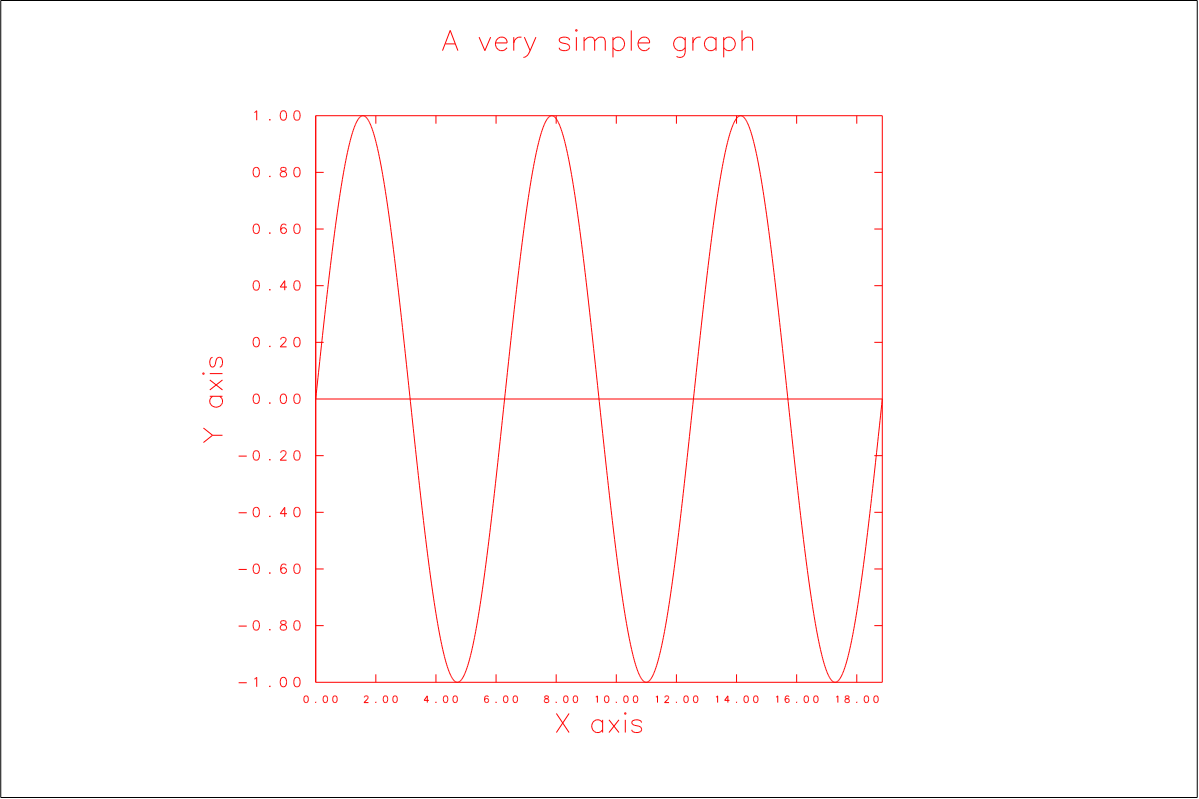
\includegraphics[width=\maxwidth]{../../temp/gr1001.eps}
  \caption{A very simple graph}
  \label{fig:gr1001}
\end{figure}

Let's start by plotting a very simple graph -- Figure \ref{fig:gr1001}.
Normally, data to be
plotted exists in disk files, but, in this first example, the data
will be internally generated by the \texttt{MEMTEST} command, which dynamically
allocates data arrays on NOS (static arrays are used on ``Unix-like'' systems)
and fills X,Y values with a sine wave.

\newpara
The script file (obey file) to generate this contains:
\begin{lstlisting}
# SIMPLEST GRAPH
#
RESET
MEMTEST
TITLE "A*L VERY SIMPLE GRAPH"
XLABEL "X*L AXIS"
YLABEL "Y*L AXIS"
XYLINE
\end{lstlisting}

\newpara
Although very minimal, there are a few points worth noting.

\begin{itemize}
\item For maximum NOS / ``Unix'' compatibility, it is best to use only UPPER CASE in obey files.
If you use lower case, it will work on both systems, but the results may be different. 
NOS (in \texttt{NORMAL} mode) will internally convert lower case to upper case. 
So ``A very simple graph'' will appear exactly as that on ``Unix'', but as ``A VERY SIMPLE GRAPH'' on NOS. 
Using upper case and \textbf{DIMFILM} ``string markup'' is portable and handles subscripts, superscripts, 
fractions and so on too. Note that \textbf{GPLOT} should \emph{not} be used in \texttt{ASCII} mode on NOS! 
\textbf{GPLOT} does not attempt to deal with 6/12 Display Code, but will convert it (mostly!) to upper case. 
However, internal arrays are not sized for 6/12 representations, so there will be problems 
(mainly strings being unexpectedly truncated rather than crahses, though).
\item The \texttt{RESET} command re-establishes a default state. If multiple obey files are used in one \textbf{GPLOT} session
without using \texttt{RESET} at the top of each file, the results will be unpredictable (the state 
at the end on one obey file will be inherited by the next).
\item This script is device independent. It can be used ``as is'' with any of the supported devices.
To generate SVG from it, we can use:
\begin{lstlisting}
/ GPLOT or $ UGPLOT
? dev svg sveg 1200,800
? prefix obey-files
? obey obgraf1
? ex
\end{lstlisting}
which will create an SVG file called \texttt{sveg001} (\texttt{sveg001.svg} on ``Unix'') using a 
``resolution'' of 1200 by 800 pixels (with SVG, this is
really a ``size'' rather than a resolution, as the vector data can be scaled without losing detail).
\item The various annotations associated with a graph (title, axis labels, etc.) should appear before the command which plots the data
(\texttt{XYLINE} here).
\item The ranges of the X and Y axes are automatically determined from the supplied data.
\item The graph is drawn in a square area in the center of the output device ``canvas''. 
When plotting graphs, it is often better to fill the output canvas.
\item Everything is drawn in a single colour (red).
\end{itemize}

\newpara
We will address these last two deficiencies in the next example.

\subsection{Bounds, panes, devices and coordinate systems in \textbf{DIMFILM}}

\newpara
It is perhaps worth understanding why the graph appears in a centered square area on the device
even at this stage. 

\newpara
\textbf{DIMFILM} lets the user define a ``world coordinate system'' or ``user coordinates''.
These ``bounds''
are defined by four numbers,
\texttt{xlo} to \texttt{xhi} defining a range of X coordinates, and
\texttt{ylo} to \texttt{yhi} defining a range of Y coordinates. This
coordinate system is intended to be ``square'' in that a unit step in X
should have the same length when drawn by the output device as a unit
step in Y. The output devices each have their own ranges of valid
coordinates. In the case of the interactive devices (\textbf{GTerm} and the
Tektronix 4014), these ranges are fixed (not strictly true for \textbf{GTerm}).
The valid range of coordinates can be set by the user for the ``file''
devices, SVG and EPS, by defining the ``paper size'' when the device is
opened. The coordinate systems of these devices are also defined to be
``square''.

\newpara
\textbf{DIMFILM} also has the concept of a ``pane'', which is initially identical
to the ``bounds''. The ``pane'' is a rectangular subregion of the
bounds, specified by four numbers in bounds coordinates.

\newpara
For general purpose drawing, you want to have a ``square'' coordinate
system, so that circles when drawn are circles and not ellipses.

\newpara
For plotting graphs of data, though, ``squareness'' is not usually
important. \textbf{DIMFILM} determines the locations and sizes of the various
elements of a graph in terms of fractions of the pane. The graph will be
placed inside the pane, squashed and stretched as may be to fill it.

\newpara
The default initial bounds (and pane) are set to 0 to 1 by 0 to 1, which
is a square region. To maintain ``squareness'' while maximising the use
of the display area, the bounds region must cover either the height or
the width of the display (or both).

\newpara
To make the situation clearer, we can draw the limits of the device
(which we have set to a 1200 by 800 ``pixel'' region when we opened the
SVG device) and the outline of the bounds (and pane) region by adding
these commands:

\begin{lstlisting}
OUTLINE DEVICE
OUTLINE BOUNDS
\end{lstlisting}

\newpara
(see Figure~\ref{fig:gr1a001}).

\begin{figure}
  \centering
  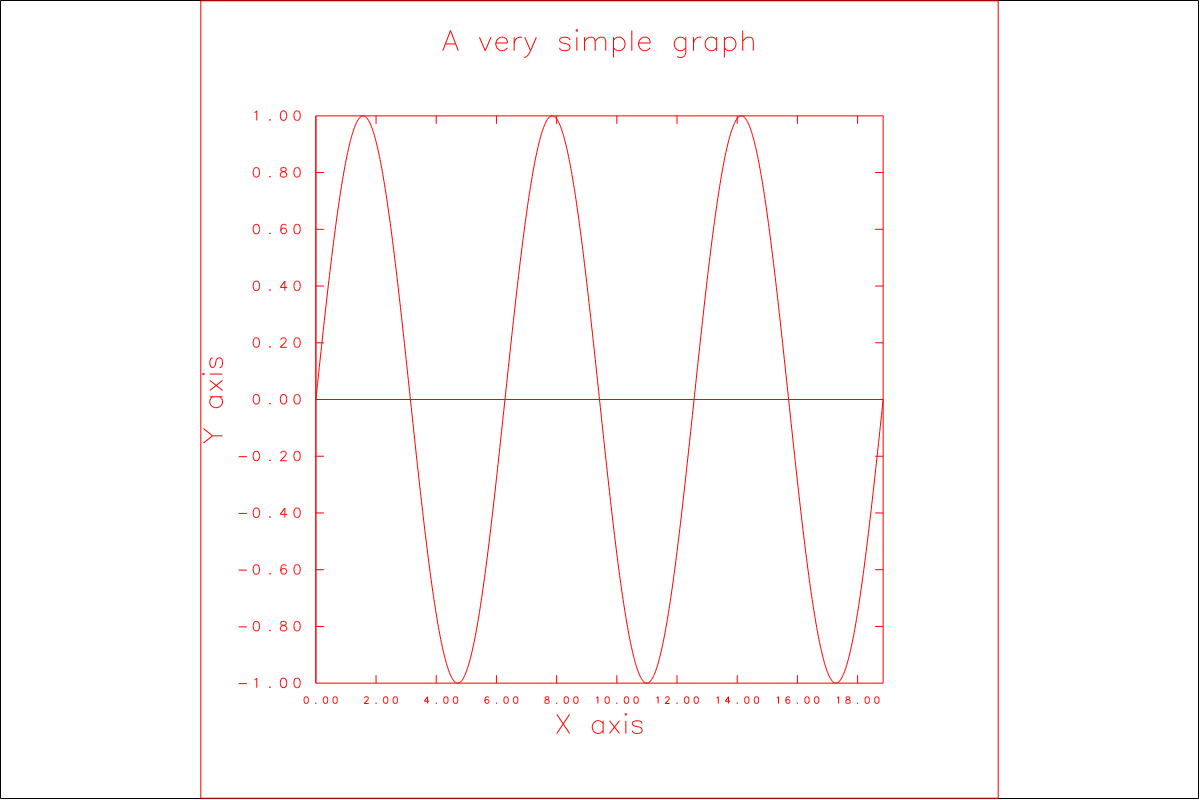
\includegraphics[width=\maxwidth]{../../temp/gr1a001.eps}
  \caption{A simple graph showing the bounds}
  \label{fig:gr1a001}
\end{figure}

\newpara
The only way to use the full area of the display is for the bounds to
have the same \emph{aspect ratio} as the display. That is:

\begin{lstlisting}
xhi - xlo     width_display
---------  =  -------------
yhi - ylo     height_display
\end{lstlisting}

\subsection{NOS, Unix-like systems and compatibility}\label{nos-unix-like-systems-and-compatibility}
\newpara
Before moving on, it may be worth discussing how \textbf{GPLOT} tries to maximise
compatability between these two very different operating systems.

\newpara
Perhaps the most obvious thing when glancing at the first example is
that the script is entirely UPPER CASE. This need not be so, and the
following will work on both ``Unix-like'' systems and NOS (although
after transfer to NOS without using 6/12 coding - which should not be
used - it will appear in upper case there).

\begin{lstlisting}
# Simplest graph.
#
reset
memtest
title "A very simple graph"
xlabel "X axis"
ylabel "Y axis"
xyline
outline dev
\end{lstlisting}

\newpara
On ``Unix-like'' systems, the output will be identical to the first
script's output. However, on NOS, the title and labels will appear in
upper case.

\newpara
Using \textbf{DIMFILM's} ``string markup sequences'' (the \texttt{*L} here)
allows lower case to be plotted on NOS.

\newpara
If you really don't like using upper case for some reason, you can use
lower case and ``string markup'' and get the same result as using upper
case on both systems.

\newpara
\textbf{GPLOT} also tries to use heuristics to make file name related matters
transparent, although there are limits to this considering each NOS
account has a flat file system with maximum 7 letter/digit upper case
only file names!

\newpara
For NOS / ``Unix'' compatibilty, you will have to stick to 7 character
file names. However, you can specify a path for ``Unix'' that is
prefixed to each file name using the \texttt{PREFIX} command. This
prefix is not used for device output files, though, so they will be
created in the current working directory.

\newpara
If you don't care about NOS compatibility, you can use long file names,
so long as the entire path name does not exceed 72 characters.

\newpara
Note that NOS does not have file name extensions. In contrast,
``Unix-like'' systems pretty much rely on having file name extensions.
EPS output files will be given \texttt{.eps} extensions on ``Unix'' and
SVG files \texttt{.svg}. These should not be added to the file names you
type in or put in scripts.

\newpara
To help identify what files contain on NOS, I use the first two
characters as a sort of ``extension'' -- e.g.~\texttt{OB} for obey files
-- but this is just a personal convention which NOS knows nothing about.

\newpara
\textbf{GPLOT} converts all supplied file names (including any \texttt{PREFIX})
to lower case on ``Unix''. You cannot use upper or mixed case file names
in \textbf{GPLOT} on ``Unix''. This applies to all input and output files. Very
rarely, this will be undesirable, but it almost always simplifies
matters. On NOS, all file names are upper case and all lower case is
converted to upper case by NOS.

\subsection{Using different colours and filling the canvas}\label{using-different-colours-and-filling-the-canvas}
\newpara
Here is the same graph as above, but with different classes of things in
different colours and filling the output canvas (Figure~\ref{fig:gr2001}).

\begin{figure}
  \centering
  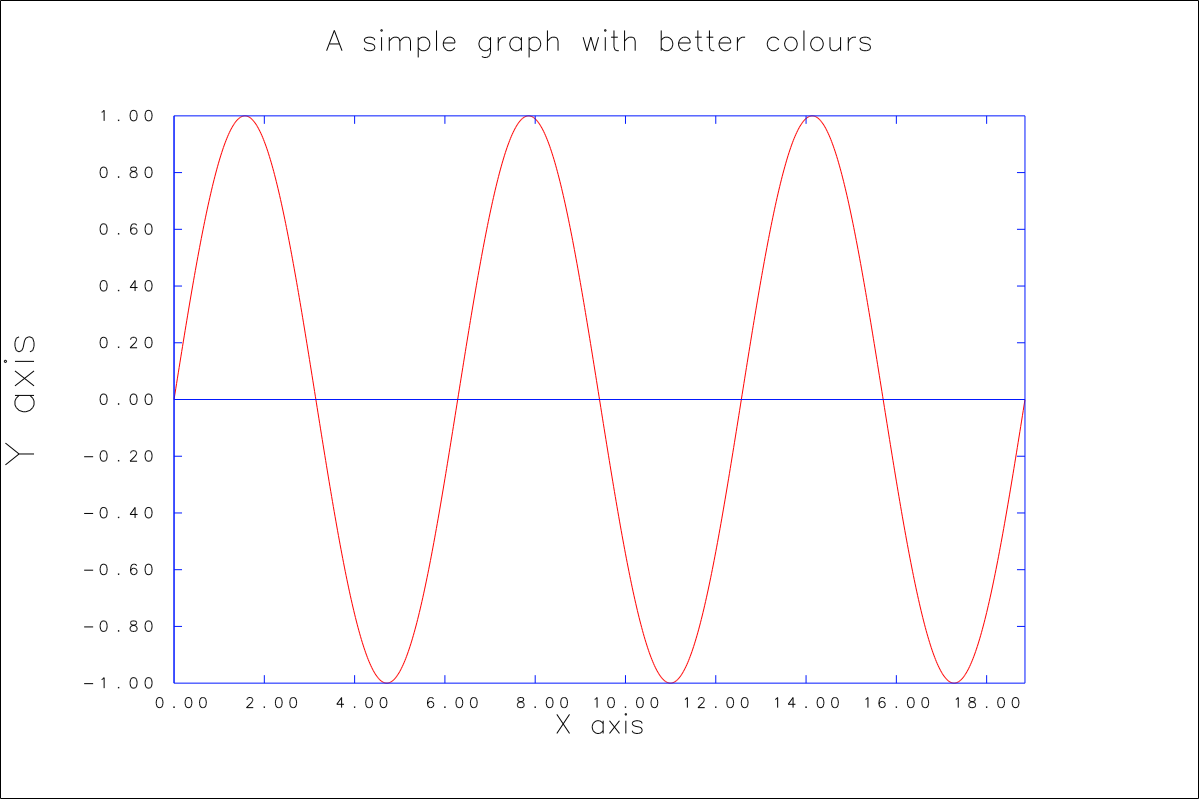
\includegraphics[width=\maxwidth]{../../temp/gr2001.eps}
  \caption{Better colours, filling the bounds}
  \label{fig:gr2001}
\end{figure}

\newpara
The code for this is:
\begin{lstlisting}
# USING COLOUR/STYLE GROUPS
#
RESET
GRAPHMODE ON
MEMTEST
CSGROUP GENERAL
COL 1 0 0
CSG TEXT
COL 0 0 0
CSG ANNOT
COL 0 0.1 1
TITLE "A*L SIMPLE GRAPH WITH BETTER COLOURS"
XLABEL "X*L AXIS"
YLABEL "Y*L AXIS"
XYLINE
OUTLINE DEV
\end{lstlisting}

\newpara
To use the full area of the device, the command:
\begin{lstlisting}
GRAPHMODE ON
\end{lstlisting}

\newpara
was added. This just sets the bounds to have the same aspect ratio as
the display device internally. In this case, to match the aspect ratio
of 1200 by 800 (3:2), the bounds will be set to 0 to 1.5 by 0 to 1.

\newpara
Note that
\begin{lstlisting}
GRAPHMODE OFF
\end{lstlisting}
resets the bounds to 0 to 1 by 0 to 1 and if bounds are explicitly
specified, they just supersede the ones set by \texttt{GRAPHMODE}.

\newpara
In \textbf{GPLOT/DIMFILM} there are 3 ``different classes of things'', namely:
\begin{itemize}
\item
  Text (\texttt{TEXT}): this refers to all types of ``strings''.
\item
  Annotation (\texttt{ANNOT}): this refers to the various things that
  annotate graphs specifically.
\item
  Other (\texttt{GENERAL}): All elements not in the above classes. This
  includes all lines and points.
\end{itemize}
All of them are members of the class \texttt{ALL}.

\newpara
These 3 classes are called ``colour/style groups'' and the current class
is selected with the \texttt{CSGROUP} command. Following this,
\texttt{COLOUR} and \texttt{WIDTH} commands set the colour (as
normalised RGB) and line width for that \texttt{CSGROUP} only. Perhaps
oddly, the line style (solid, dashed, etc.) is \emph{not} set
independently for different groups. The current line style applies to
all groups.

\newpara
Note that any command can be abbreviated -- so long as the abbreviation
remains unique, it will work. (Note that this is \emph{not} true of
evaluator operators, as we will see).


\subsection{Adding a grid or graticule}\label{adding-a-grid-or-graticule}
\newpara
In order to better see the values on plotted graphs, it is often useful
to have a grid or graticule over which the graphs are plotted (as with
traditional graph paper). This is easily added with the \texttt{GRID}
command:

\begin{lstlisting}
# ADD A GRID
#
RESET
GRAPHMODE ON
MEMTEST
CSGROUP GENERAL
COL 1 0 0
CSG TEXT
COL 0 0 0
CSG ANNOT
COL 0 0.1 1
TITLE "A*L SIMPLE GRAPH WITH A GRID"
XLABEL "X*L AXIS"
YLABEL "Y*L AXIS"
GRID BOTH
XYLINE
OUTLINE DEV
\end{lstlisting}

\newpara
resulting in Figure~\ref{fig:gr3001}.

\begin{figure}
  \centering
  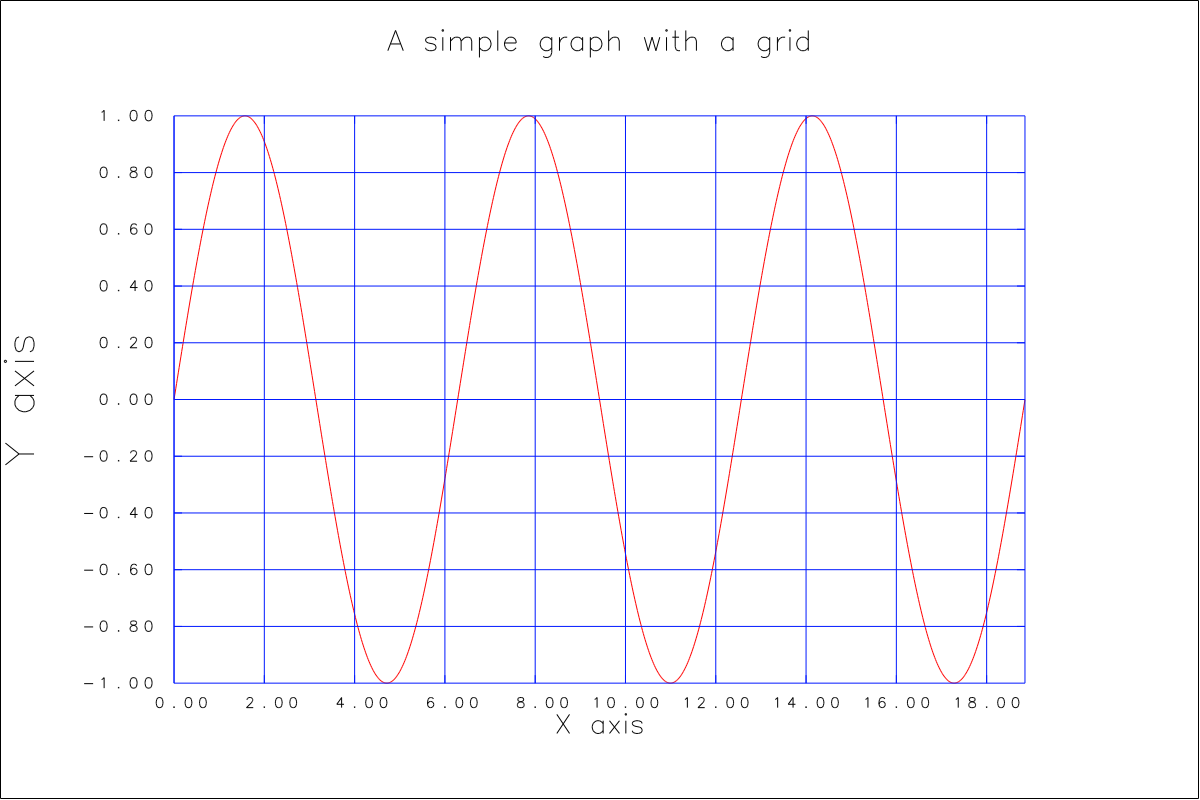
\includegraphics[width=\maxwidth]{../../temp/gr3001.eps}
  \caption{Adding a grid}
  \label{fig:gr3001}
\end{figure}


\subsection{Changing the width of lines}\label{changing-the-width-of-lines}
\newpara
As with colour, the width of lines can easily be set independently for
each colour/style group with the \texttt{WIDTH} command. As an example,
see Figure~\ref{fig:gr4001}.

\begin{lstlisting}
# GRAPH PLOT WITH WIDER LINE
#
RESET
MEMTEST
GRAPHMODE ON
CSGROUP GENERAL
COL 1 0 0
WIDTH 3
CSG TEXT
COL 0 0 0
CSG ANNOT
COL 0 0.1 1
TITLE "A*L SIMPLE GRAPH WITH A WIDER LINE"
XLABEL "X*L AXIS"
YLABEL "Y*L AXIS"
GRID BOTH
XYLINE
OUTLINE DEV
\end{lstlisting}

\begin{figure}
  \centering
  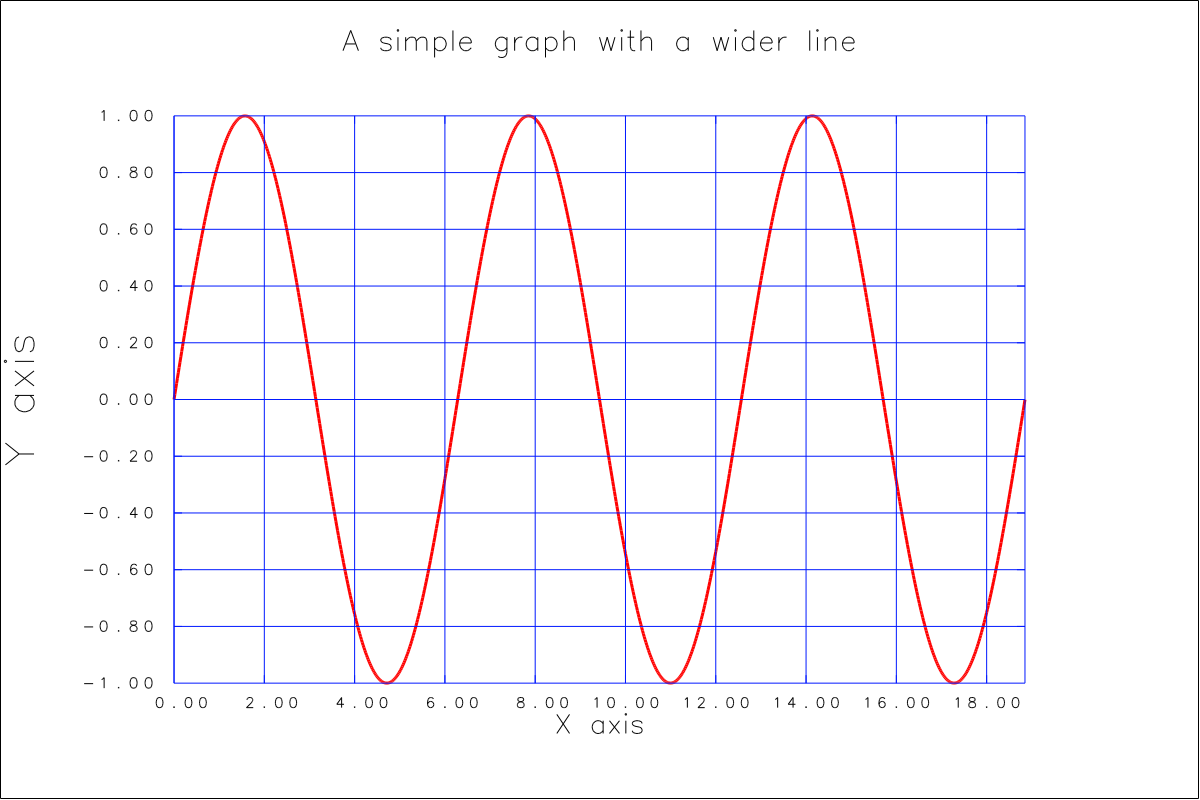
\includegraphics[width=\maxwidth]{../../temp/gr4001.eps}
  \caption{Adjusting line width}
  \label{fig:gr4001}
\end{figure}

\subsection{Different graph styles}\label{different-graph-styles}
\newpara
The graphs above are all drawn with the default ``framed'' graph style.
An alternative is the ``open'' style, shown in Figure~\ref{fig:gr5001}.

\begin{lstlisting}
# OPEN STYLE GRAPH
#
RESET
MEMTEST
GRAPHMODE ON
CSGROUP GENERAL
COL 1 0 0
WIDTH 3
CSG TEXT
COL 0 0 0
CSG ANNOT
COL 0 0.1 1
GSTYLE OPEN
TITLE "A*LN OPEN STYLE SIMPLE GRAPH"
XLABEL "X*L AXIS"
YLABEL "Y*L AXIS"
XYLINE
OUTLINE DEV
\end{lstlisting}

\begin{figure}
  \centering
  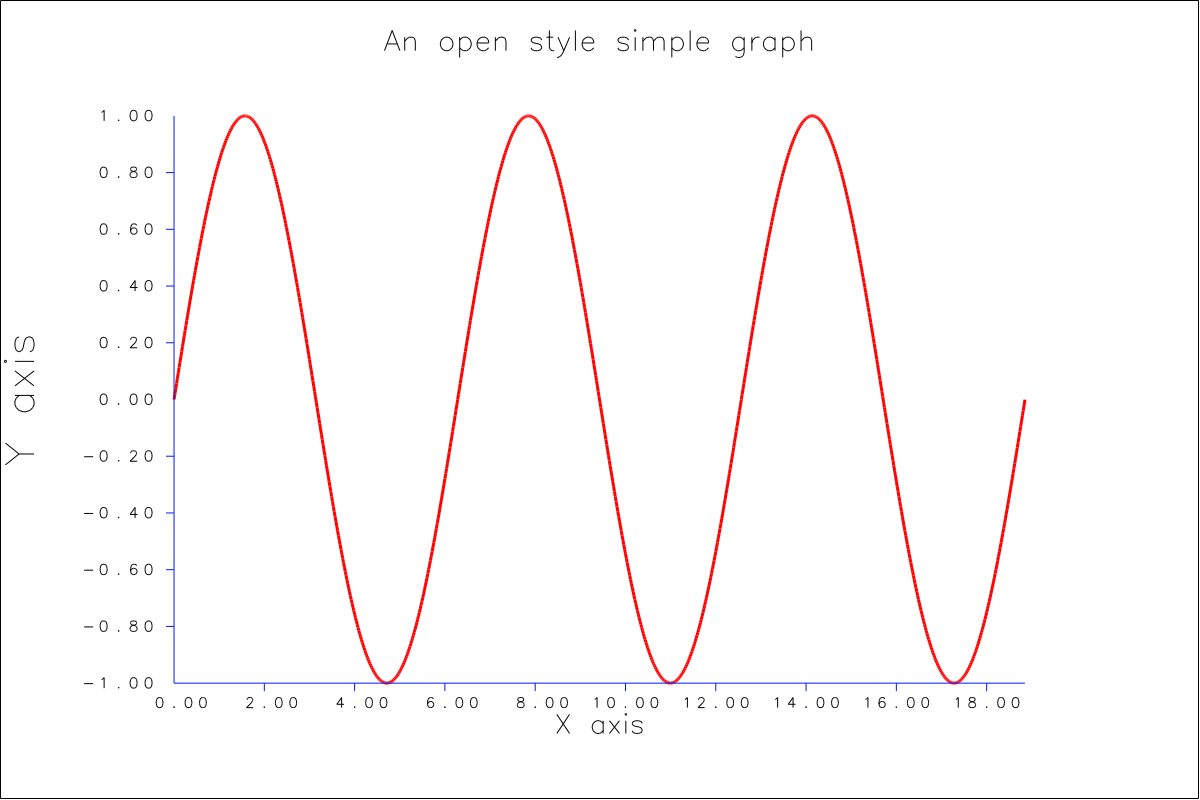
\includegraphics[width=\maxwidth]{../../temp/gr5001.eps}
  \caption{Open style graph}
  \label{fig:gr5001}
\end{figure}

\newpara
Another alternative is the ``axes'' style, as shown in Figure~\ref{fig:gr7001}.

\begin{figure}
  \centering
  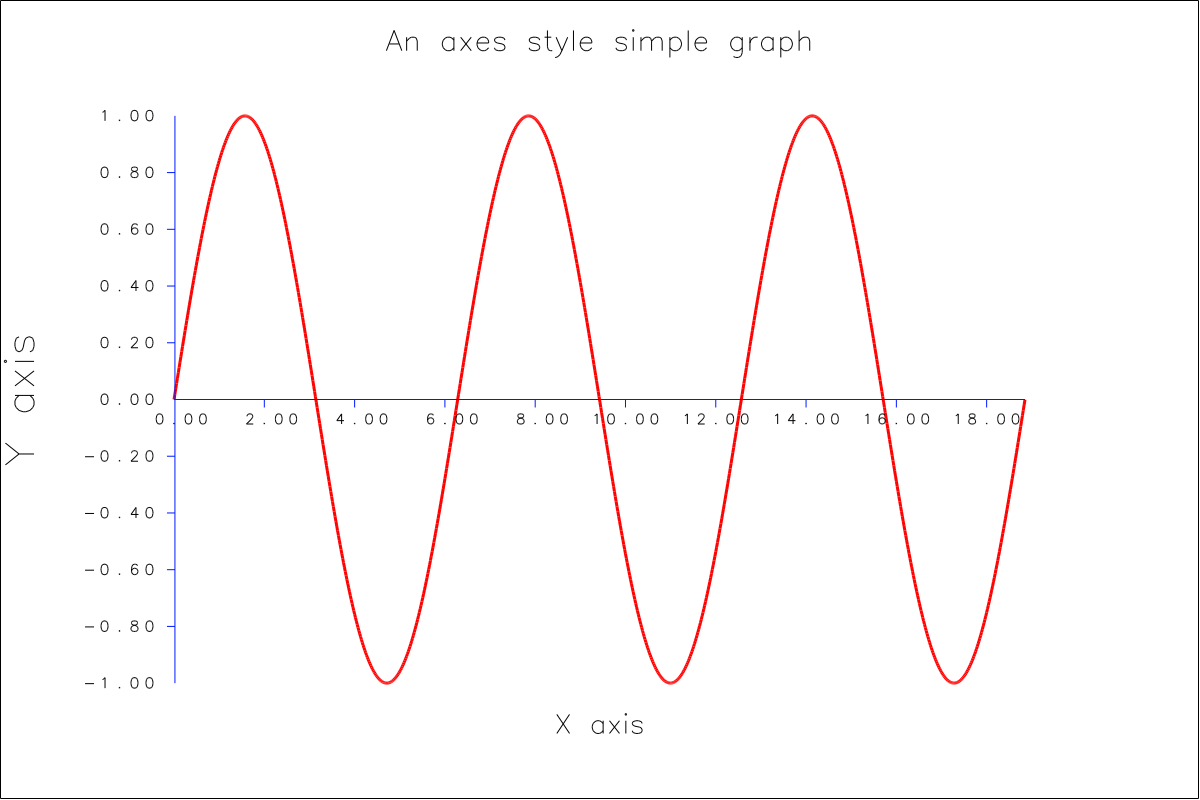
\includegraphics[width=\maxwidth]{../../temp/gr7001.eps}
  \caption{Axes style graph}
  \label{fig:gr7001}
\end{figure}

\begin{lstlisting}
# AXES STYLE GRAPH
#
RESET
MEMTEST
CSGROUP GENERAL
COL 1 0 0
WIDTH 3
CSG TEXT
COL 0 0 0
CSG ANNOT
COL 0 0.1 1
AXCUT 0.02 0
GSTYLE AXES
TITLE "A*LN AXES STYLE SIMPLE GRAPH"
XLABEL "X*L AXIS"
YLABEL "Y*L AXIS"
XYLINE
OUTLINE DEV
\end{lstlisting}

\newpara
To which a grid can be added in the obvious way (Figure~\ref{fig:gr8001}).

\begin{figure}
  \centering
  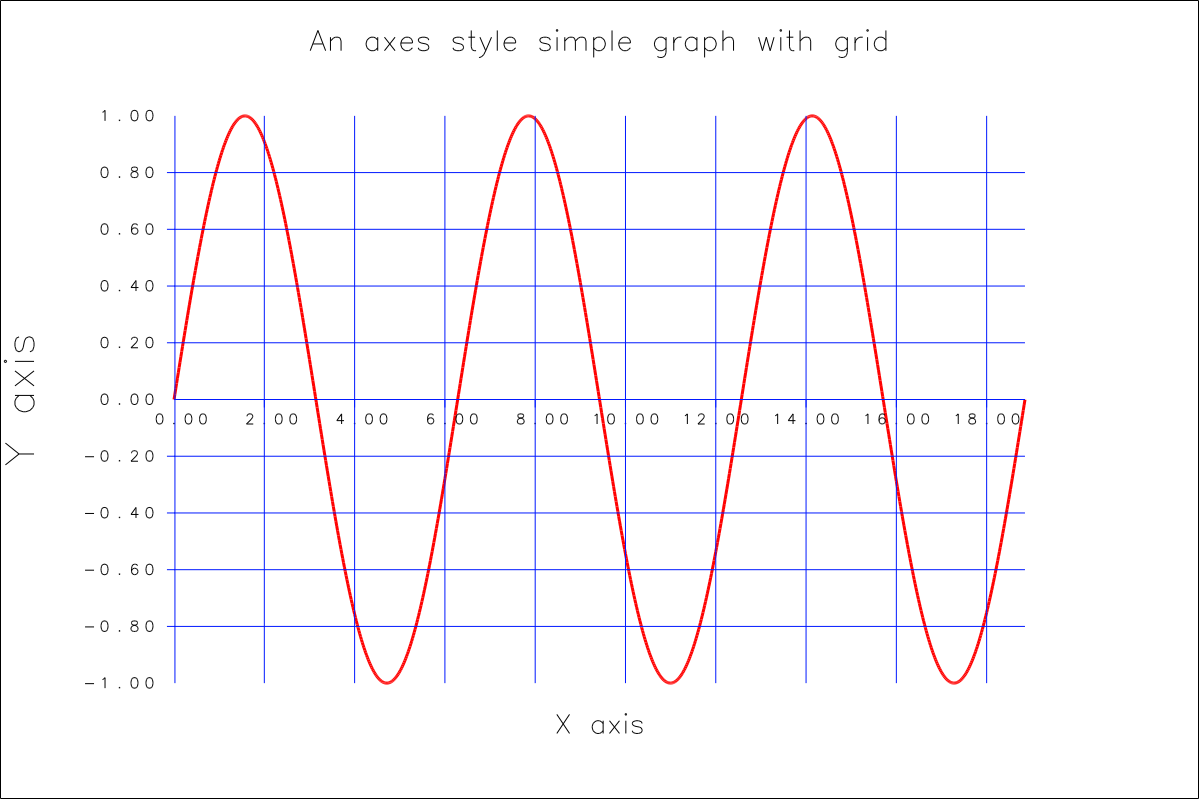
\includegraphics[width=\maxwidth]{../../temp/gr8001.eps}
  \caption{Adding a grid}
  \label{fig:gr8001}
\end{figure}

\begin{lstlisting}
# AXES STYLE GRAPH WITH GRID
#
RESET
GRAPHMODE ON
MEMTEST
CSGROUP GENERAL
COL 1 0 0
WIDTH 3
CSG TEXT
COL 0 0 0
CSG ANNOT
COL 0 0.1 1
AXCUT 0.02 0
GSTYLE AXES
GRID BOTH
TITLE "A*LN AXES STYLE SIMPLE GRAPH WITH GRID"
XLABEL "X*L AXIS"
YLABEL "Y*L AXIS"
XYLINE
OUTLINE DEV
\end{lstlisting}


\subsection{Multiple graphs on the same axes and ``HERE'' data}\label{multiple-graphs-on-the-same-axes-and-here-data}
\newpara
To plot more than one graph on the same axes is quite straightforward.
First, note that we haven't explicitly specified the ranges of the axes
in any of the graphs so far. Instead, the system has looked at the data
and automatically found reasonable ranges for the axes. This is very
often the best approach.

\newpara
To plot more than one graph and keep automatically determining the axis
ranges can be done with the with two commands: \texttt{XYSAME} and
\texttt{ANNOT\ OFF}. The second prevents annotation being drawn multiple
times and the first keeps the axis ranges automatically determined from
the first data plotted.

\newpara
\textbf{GPLOT} also lets you specify data ``inline'' in a script file. Here is a
very simple example (Figure~\ref{fig:gr10001}) and the script that generated it.

\begin{figure}
  \centering
  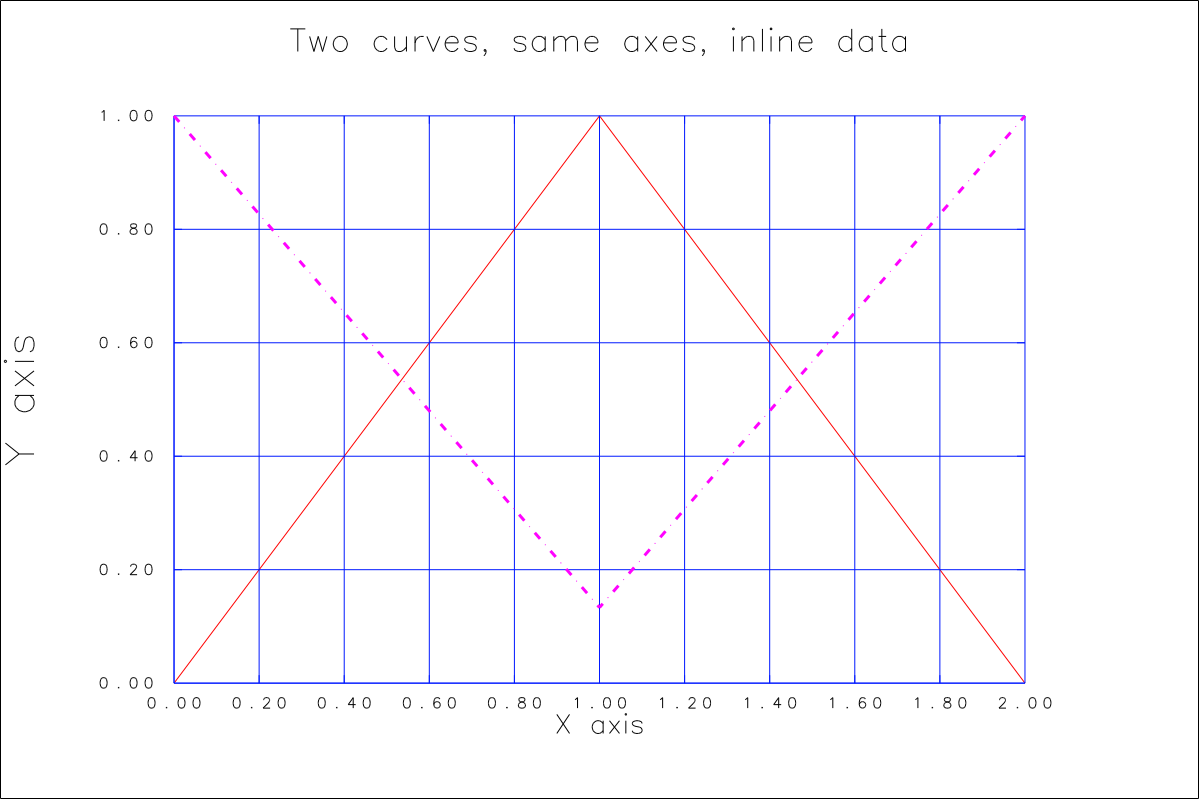
\includegraphics[width=\maxwidth]{../../temp/gr10001.eps}
  \caption{Multiple graphs, same axes}
  \label{fig:gr10001}
\end{figure}

\begin{lstlisting}
# 2 CURVE GRAPH WITH INLINE DATA
#
RESET
#
GRAPHMODE ON
GSTYLE BOXED
#
CSGROUP GENERAL
COL 1 0 0
WIDTH 1
STYLE SOLID
#
CSG TEXT
COL 0 0 0
STYLE SOLID
#
CSG ANNOT
COL 0 0.1 1
STYLE SOLID
#
#--- DEFINE SOME DATA INLINE 
READ HERE 1 2
0 0
1 1
2 0
EOF
#--- DRAW THAT WITH AUTO DETERMINED AXIS RANGES
GRID BOTH
TITLE "T*LWO CURVES, SAME AXES, INLINE DATA"
XLABEL "X*L AXIS"
YLABEL "Y*L AXIS"
XYLINE
#
#--- TURN OFF ANNOTATION AND KEEP AUTO DET RANGES FOR NEXT CURVE
ANNOT OFF 
XYSAME
#
#--- DEFINE SOME MORE DATA INLINE
READ HERE 1 2
0 1
1 0.1333
2 1
EOF
#
#--- DRAW THAT IN A DIFFERENT COLOUR AND WIDTH.
CSG GEN
COL 1 0 1
WIDTH 3
STYLE DASHDOT
XYLINE
OUTLINE DEVICE
\end{lstlisting}

\newpara
Note the \texttt{READ} command. This is described further in the section
on plotting data in files. For inline data, the keyword \texttt{HERE} is
used with it, and the data follows immediately. That data is terminated
by \texttt{EOF}. The numeric arguments to \texttt{READ} are ``column
numbers'' and will almost always be \texttt{1\ 2} for inline data.

\subsection{Multiple graphs and keys}\label{multiple-graphs-and-keys}
\newpara
\textbf{GPLOT} provides a straightforward (if inflexible) way of adding a key or
legend to help identify the meaning of the lines (or points) on graphs.

\newpara
Figure~\ref{fig:gr11001} is an example of three curves with a key and the generating script.
The data is again defined by ``HERE'' data.

\begin{figure}
  \centering
  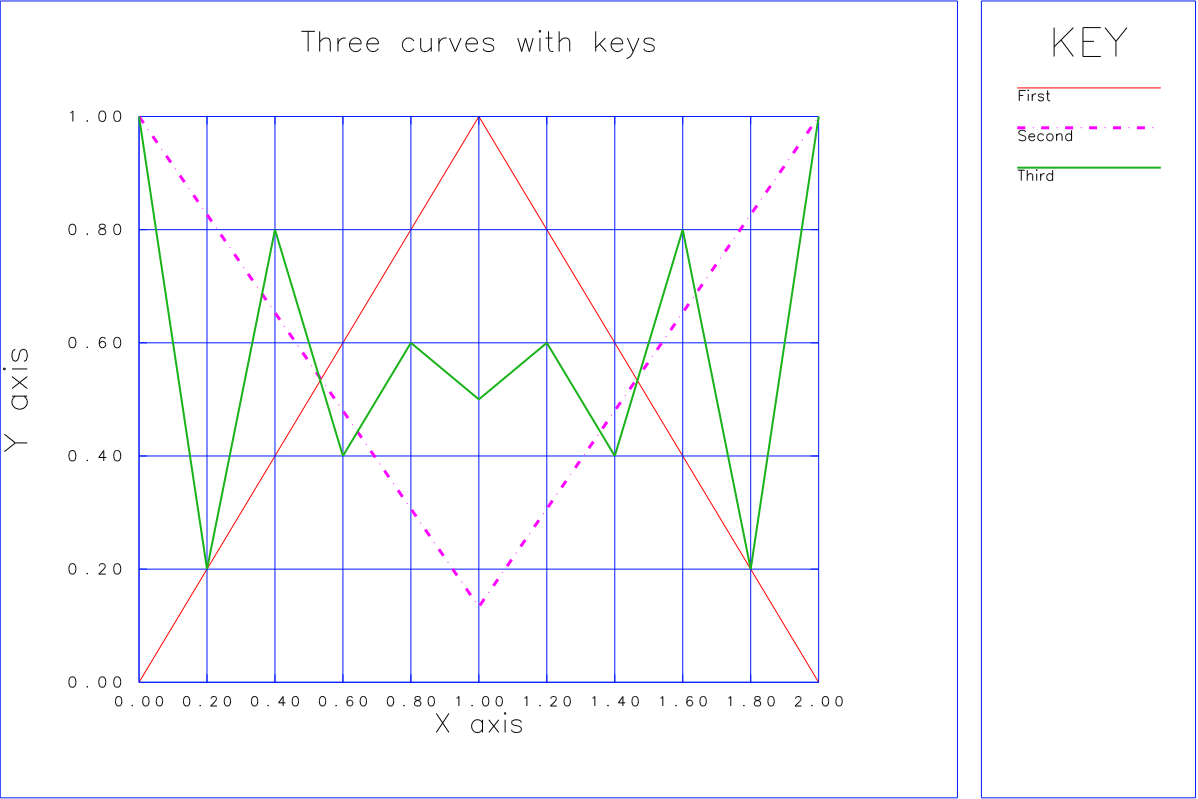
\includegraphics[width=\maxwidth]{../../temp/gr11001.eps}
  \caption{Multiple graphs with a key}
  \label{fig:gr11001}
\end{figure}

\begin{lstlisting}
# 3 CURVE GRAPH WITH INLINE DATA AND KEYS
#
RESET
GRAPHMODE ON
#
GSTYLE BOXED
#
CSGROUP GENERAL
COL 1 0 0
WIDTH 1
STYLE SOLID
#
CSG TEXT
COL 0 0 0
STYLE SOLID
#
CSG ANNOT
COL 0 0.1 1
STYLE SOLID
#
# --- DEFINE SOME DATA INLINE 
READ HERE 1 2
0 0
1 1
2 0
EOF
#
# --- WE WILL ADD KEYS.
USEKEY
#
# --- DRAW THAT WITH AUTO DETERMINED AXIS RANGES
GRID BOTH
TITLE "T*LHREE CURVES WITH KEYS"
XLABEL "X*L AXIS"
YLABEL "Y*L AXIS"
XYLINE
ADDKEY "F*LIRST"
#
# --- TURN OFF ANNOTATION AND KEEP AUTO DET RANGES FOR NEXT CURVE
ANNOT OFF 
XYSAME
#
# --- DEFINE SOME MORE DATA INLINE
READ HERE 1 2
0 1
1 0.1333
2 1
EOF
#
# --- DRAW THAT IN A DIFFERENT COLOUR AND WIDTH.
CSG GEN
COL 1 0 1
WIDTH 3
STYLE DASHDOT
XYLINE
ADDKEY "S*LECOND"
#
# --- DEFINE YET MORE DATA INLINE
READ HERE 1 2
0 1
0.2 0.2
0.4 0.8
0.6 0.4
0.8 0.6
1.0 0.5
1.2 0.6
1.4 0.4
1.6 0.8
1.8 0.2
2 1
EOF
#
# --- DRAW THAT IN A DIFFERENT COLOUR AND WIDTH.
CSG GEN
COL 0.1 0.7 0.1
WIDTH 2
STYLE SOLID
XYLINE
ADDKEY "T*LHIRD"
#
# --- DRAW THE LEGEND.
KEYS
OUTLINE DEV
\end{lstlisting}

\newpara
This allows adding keys for up to 20 curves (I find 10 curves on one
graph is as much as I can cope with). The maximum length of the key text
is also quite limited at a maximum of 15 characters (including any
markup sequences).

\newpara
The layout currently cannot be changed. The key/legend area is always
positioned to the right of the graph. This may be better than trying to
put the key on top of the graph, as it can be impossible to find a place
to put that without obscuring part of the data (at least, I've often
found that is the case over the decades). That approach could certainly
be added, though.

\subsubsection{Multiple curves with two different Y axis
ranges}\label{multiple-curves-with-two-different-y-axis-ranges}
\newpara
Sometimes it is useful to plot two (or more) curves with the same X axis
but, because they have significantly different Y ranges, two distinct Y
axes. This can be done by having one Y axis on the left of a graph and
another on the right.

\newpara
A simple example is shown in Figure~\ref{fig:gr12001}.

\begin{figure}
  \centering
  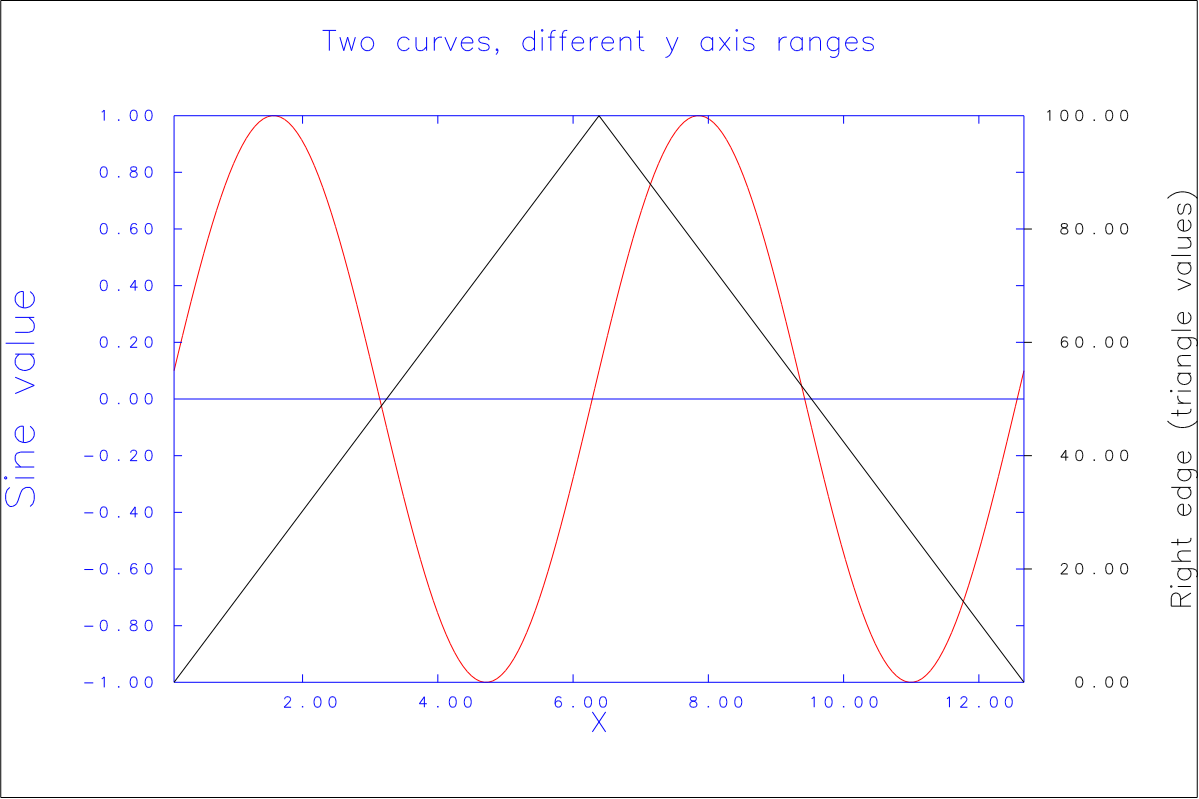
\includegraphics[width=\maxwidth]{../../temp/gr12001.eps}
  \caption{Common X axis, two different Y ranges}
  \label{fig:gr12001}
\end{figure}

\begin{lstlisting}
# TWO CURVES, DIFFERENT AXIS RANGES
#
RESET
GRAPHMODE ON
CSG ANNOT
COL 0 0 1
CSG TEXT
COL 0 0 1
#
# --- GENERATE A SINE WAVE.
EVAL 0.1,TWPI,2,*,0.1,+,201,XLIN,X,SIN
#
# --- PLOT IT WITH AUTO AXIS RANGES.
XLAB "X"
YLABEL "S*LINE VALUE"
TITLE "T*LWO CURVES, DIFFERENT Y AXIS RANGES"
XYL
ANNOT OFF
#
# --- DEFINE A TRIANGLE WAVE SHAPE.
READ HERE 1 2
0 0
5 100
10 0
EOF
#
# --- PLOT THAT WITH AUTO AXIS, PUT VALUES ON RIGHT
CSG ALL
COLOUR 0 0 0
RIGHTANNOT ON
RYLABEL "R*LIGHT EDGE (TRIANGLE VALUES)"
XYL
OUTLINE DEV
\end{lstlisting}

\newpara
This example includes the first use of the evaluator so far (to create
the sine wave curve). It is not essential to this example, though.

\newpara
Note that the axis ranges are still automatically determined
(\texttt{XYSAME} is not used for obvious reasons). The
\texttt{ANNOT\ OFF} command is need though, before the
\texttt{RIGHTANNOT} command is used.

\newpara
It is possible to create a key for such a graph too (Figure~\ref{fig:gr13001}).

\begin{figure}
  \centering
  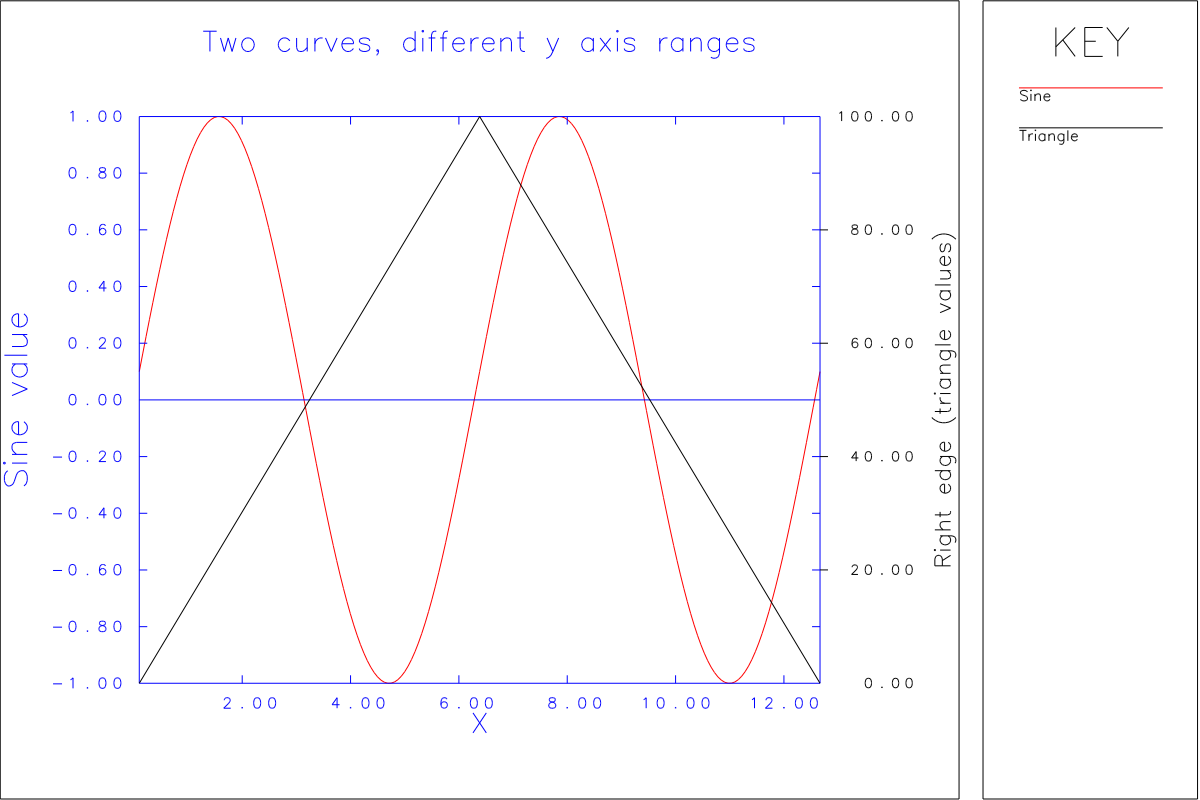
\includegraphics[width=\maxwidth]{../../temp/gr13001.eps}
  \caption{Two different Y ranges and a key}
  \label{fig:gr13001}
\end{figure}

\begin{lstlisting}
# TWO CURVES, DIFFERENT AXIS RANGES, KEY
#
RESET
GRAPHMODE ON
CSG ANNOT
COL 0 0 1
CSG TEXT
COL 0 0 1
#
# --- GENERATE A SINE WAVE.
EVAL 0.1,TWPI,2,*,0.1,+,201,XLIN,X,SIN
#
# --- WE WILL USE KEYS.
USEKEY
#
# --- PLOT IT WITH AUTO AXIS RANGES.
XLAB "X"
YLABEL "S*LINE VALUE"
TITLE "T*LWO CURVES, DIFFERENT Y AXIS RANGES"
XYL
ADDKEY "S*LINE"
ANNOT OFF
#
# --- DEFINE A TRIANGLE WAVE SHAPE.
READ HERE 1 2
0 0
5 100
10 0
EOF
#
# --- PLOT THAT WITH AUTO AXIS, PUT VALUES ON RIGHT
CSG ALL
COLOUR 0 0 0
RIGHTANNOT ON
RYLABEL "R*LIGHT EDGE (TRIANGLE VALUES)"
XYL
ADDKEY "T*LRIANGLE"
#
# --- DRAW LEGEND.
KEYS
OUTLINE DEV
\end{lstlisting}

\subsection{Plotting data stored in a disk file}\label{plotting-data-stored-in-a-disk-file}
\newpara
So far, we have plotted data that has been generated by \textbf{GPLOT} or stored
as ``HERE'' data in the command stream. Very often, the data to be
plotted will be in disk files, though.

\newpara
\textbf{GPLOT} provides a very simple, albeit basic, way of reading such data and
plotting it. Given a file containing the same number of numeric items on
each line, with those items separated by spaces or a comma (and perhaps
spaces), \textbf{GPLOT} can treat the n-th number on each line as an entry in a
column of numbers. The columns are numbered 1, 2, 3, etc.

\newpara
Any line that begins with \texttt{\#} or \texttt{C} (upper case C, not
lower case) will be skipped as a comment. Any entirely blank lines will
also be skipped.

\newpara
The \texttt{READ} command is followed by the name of the data file to be
read then the column numbers for the X and Y coordinates.

\newpara
Figure~\ref{fig:gr14001} is an example of some real measured data stored in a file
(\texttt{DAEG1}) and plotted.

\begin{figure}
  \centering
  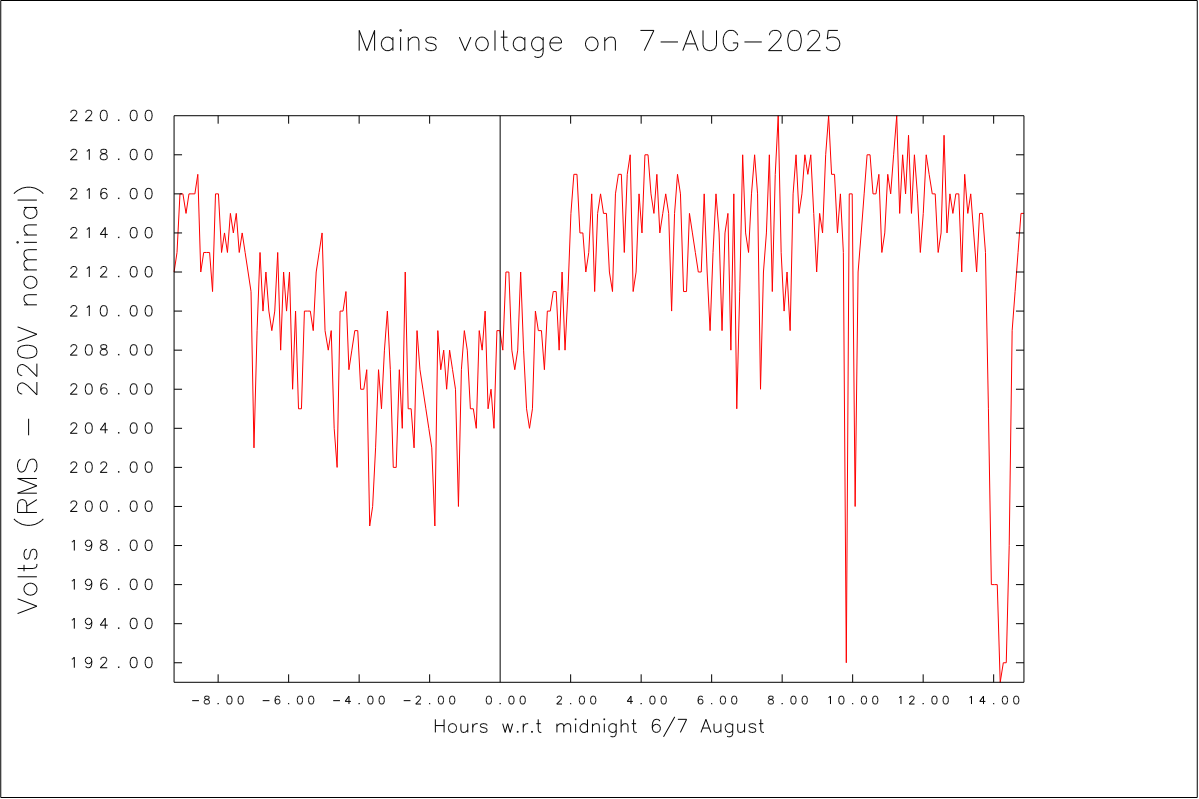
\includegraphics[width=\maxwidth]{../../temp/gr14001.eps}
  \caption{Measured data from a file}
  \label{fig:gr14001}
\end{figure}

\begin{lstlisting}
# READ AN X,Y DATA FILE AND PLOT THE CONTENTS
#
RESET
GRAPHMODE ON
#
# --- READ THE DATA FILE, FIRST 2 COLUMNS, SPACE OR COMMA SEP.
GET DAEG1
READ DAEG1 1 2
#
# --- DRAW THE GRAPH
CSG ANNOT
COL 0 0 0
CSG TEXT
COL 0 0 0
TITLE "M*LAINS VOLTAGE ON 7-*UAUG*L-2025"
XLABEL "H*LOURS W.R.T MIDNIGHT 6/7 *UA*LUGUST"
YLABEL "V*LOLTS (*URMS - 220V *LNOMINAL)"
XYLINE
#
OUTLINE DEV
\end{lstlisting}

\newpara
The data file will usually have at least two columns. However, a single
column of data can be plotted. That data will become the Y values and
the X values will be the line number (starting at 0). Use a 0 column
number to do this. For example:

\begin{lstlisting}
READ DAEG1 0 2
\end{lstlisting}

\subsection{Labelling points on a graph}\label{labelling-points-on-a-graph}
\newpara
It is sometimes useful to point out something on a graph.
Figure~\ref{fig:gr15001} is an example of this.

\begin{figure}
  \centering
  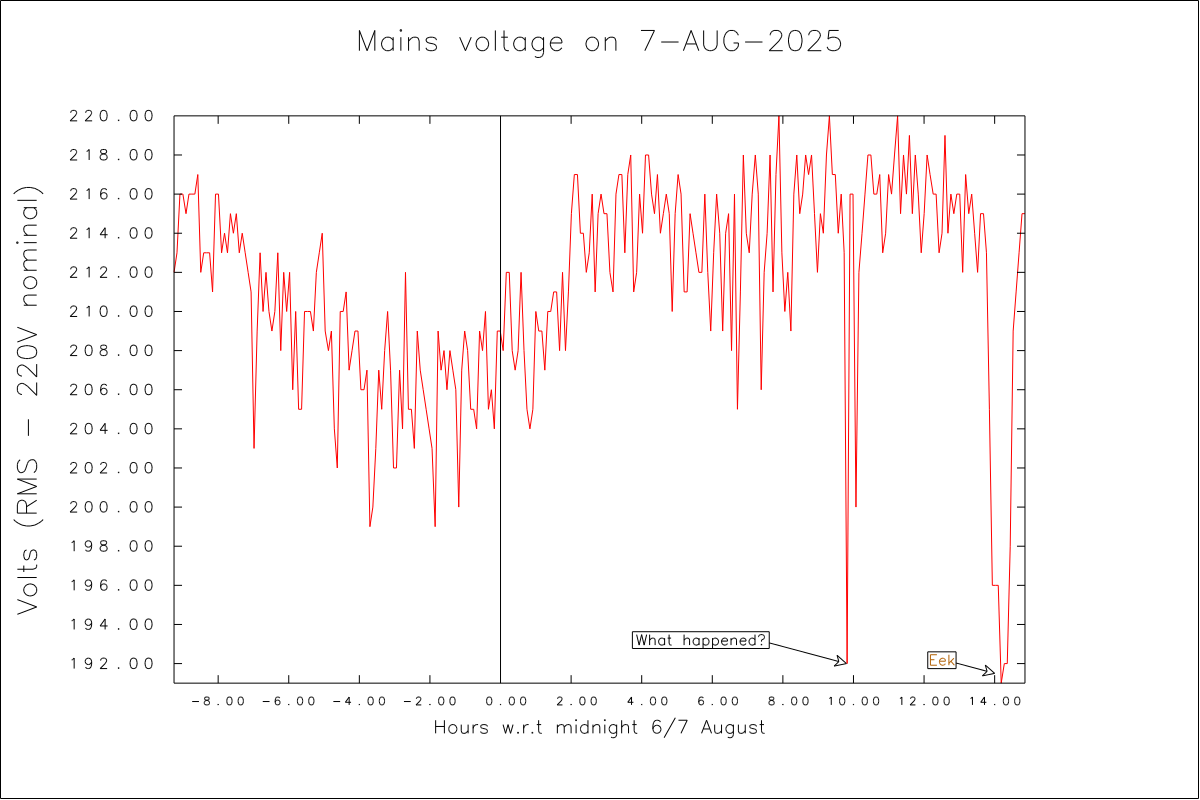
\includegraphics[width=\maxwidth]{../../temp/gr15001.eps}
  \caption{Labelling points on a graph}
  \label{fig:gr15001}
\end{figure}

\newpara
This is quite easy to do, in this case by adding the following commands
between \texttt{XYLINE} and \texttt{OUTLINE}:

\begin{lstlisting}
#
# --- ADD A LABEL OR TWO
CSG ALL
COL 0 0 0
GLABEL 9.8 192.0 0.1 165 "W*LHAT HAPPENED?"
CSG TEXT
COL 0.7 0.384 0.025
GLABEL 14 191.5 0.05 165 "E*LEK"
\end{lstlisting}

\newpara
The \texttt{GLABEL} command's first two arguments are the graph
coordinates to which the label's arrow should point. The third argument
is the length of the arrow in \emph{bounds coordinates} (which will be 0
to 1 by 0 to 1 by default, or 0 to (device aspect ratio) by 0 to 1 if
\texttt{GRAPHMODE\ ON} is in effect). The fourth argument is the angle
of the arrow around the location it is pointing at, counter-clockwise
from \texttt{+X} in degrees. The final argument is the text for the
label, which will be drawn in a box at the blunt end of the arrow.

\subsection{Data with uncertainties (error bars) in Y}\label{data-with-uncertainties-error-bars-in-y}
\newpara
If your data has an uncertainty measure associated with it, that can be
plotted as an error bar on the graph. The meaning of this value is
entirely up to you, of course. For common meanings see this
\href{https://en.wikipedia.org/wiki/Error_bar}{Wikipedia article}.

\newpara
Using a concocted data file (\texttt{DAEG2}) which looks like this:

\begin{lstlisting}
0.0,0.0,0.0
0.1,0.01,0.004
0.2,0.04,0.01
0.3,0.09,0.041
0.4,0.16,0.083
0.5,0.25,0.013
0.6,0.36,0.022
0.7,0.49,0.033
0.8,0.64,0.054
0.9,0.81,0.065
1.0,1.0,0.1
\end{lstlisting}

\newpara
(note the use of comma separated instead of blank separated values
here), the following script will plot a graph with error bar data taken
from column 3:

\begin{lstlisting}
# READ AN X,Y,E DATA FILE AND PLOT THE CONTENTS
#
RESET
GRAPHMODE ON
#
# --- READ THE DATA FILE, FIRST 3 COLUMNS. THIS ONE USES COMMAS.
GET DAEG2
READ DAEG2 1 2 3
#
# --- DRAW THE GRAPH
CSG ANNOT
COL 0 0 0
CSG TEXT
COL 0 0 0
CSG GEN
COL 0.8 0.1 0.1
TITLE "L*LOOKS LIKE X*+2$+ WITH SYMMETRICAL ERRORS"
XLABEL "X"
YLABEL "Y"
XYLINE
OUTLINE DEV
\end{lstlisting}

\newpara
This results in Figure~\ref{fig:gr16001}.

\begin{figure}
  \centering
  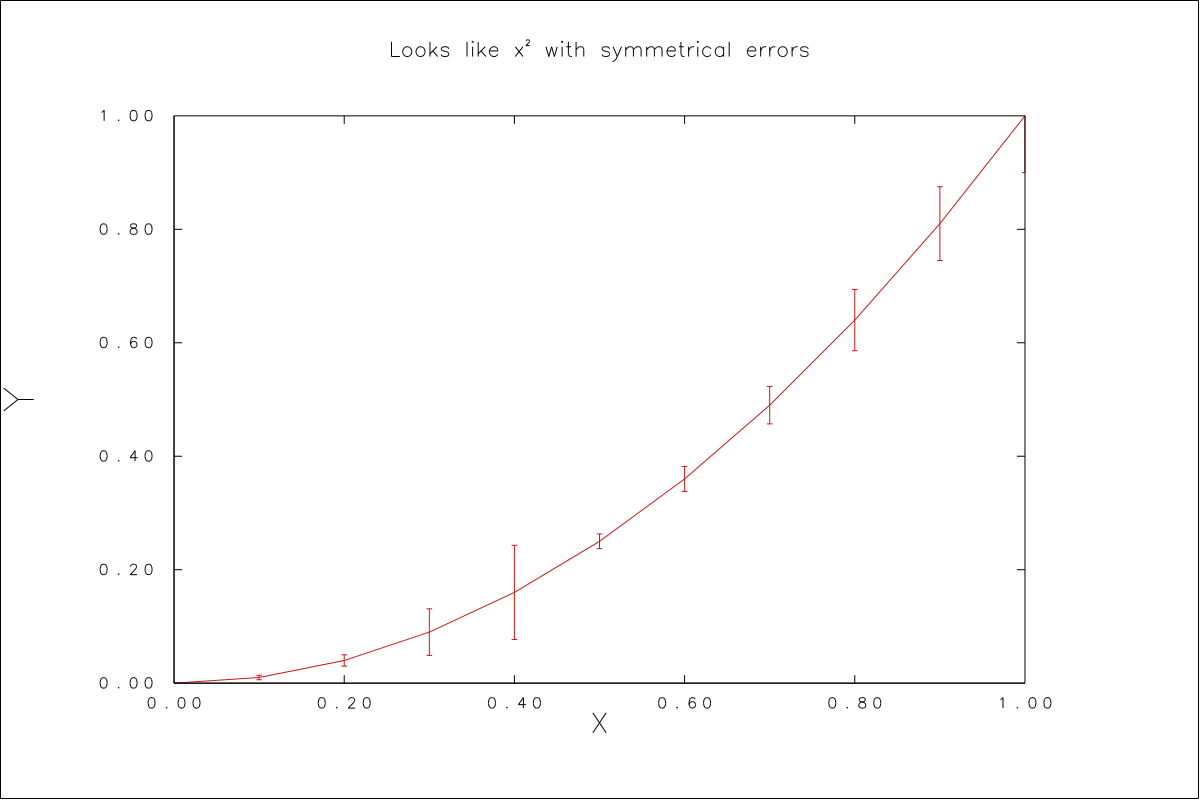
\includegraphics[width=\maxwidth]{../../temp/gr16001.eps}
  \caption{Symmetric Y error bars}
  \label{fig:gr16001}
\end{figure}

\newpara
The column given as the third argument to \texttt{READ} supplies the
delta from the values taken from the column given as the second argument
to \texttt{READ} at which error bar limits will be drawn above and below
the value.

\subsection{Data with asymmetric uncertainties in Y}\label{data-with-asymmetric-uncertainties-in-y}
\newpara
It is possible that your data has potential deviations that are larger
in the negative direction than in the positive direction, perhaps
because the underlying data distribution is not normal, but skewed, or
perhaps the device making measurements has errors that are proportional
to the magnitude of the measured values. To visualise this, you need
asymmetric error bars in Y.

\newpara
To illustrate this, we have concocted another data file
(\texttt{DAEG3}):

\begin{lstlisting}
0.0,0.0,0.0,0.0,0.0
0.1,0.01,0.004,0.006,0.002
0.2,0.04,0.01,0.12,0.033
0.3,0.09,0.041,0.032,0.092
0.4,0.16,0.083,0.043,0.161
0.5,0.25,0.013,0.09,0.251
0.6,0.36,0.022,0.022,0.3617
0.7,0.49,0.033,0.021,0.5
0.8,0.64,0.054,0.066,0.666
0.9,0.81,0.065,0.032,0.814
1.0,1.0,0.1,0.05,0.997
\end{lstlisting}

\newpara
Note this has 5 columns but here we will use the first four.
\newpara
To plot this with asymmetrical error bars only requires a change to
\texttt{READ}. The \texttt{XYLINE} (or \texttt{XYPOINT}) command will
plot whatever the last \texttt{READ} has read.
\newpara
Note the command: \texttt{ASYMYERRORS\ YES} which explicitly turns on
this behaviour. This is not needed, however, as it is the default.

\begin{lstlisting}
# READ AN X,Y,EU,EL DATA FILE AND PLOT THE CONTENTS
#
RESET
GRAPHMODE ON
#
# --- READ THE DATA FILE, FIRST 4 COLUMNS. THIS ONE USES COMMAS.
ASYMYERRORS YES
GET DAEG3
READ DAEG3 1 2 3 4
#
# --- DRAW THE GRAPH
CSG ANNOT
COL 0 0 0
CSG TEXT
COL 0 0 0
CSG GEN
COL 0.8 0.1 0.1
TITLE "L*LOOKS LIKE X*+2$+ WITH ASYMMETRICAL ERRORS"
XLABEL "X"
YLABEL "Y"
XYLINE
OUTLINE DEV
\end{lstlisting}

\newpara
This results in Figure~\ref{fig:gr17001}.

\begin{figure}
  \centering
  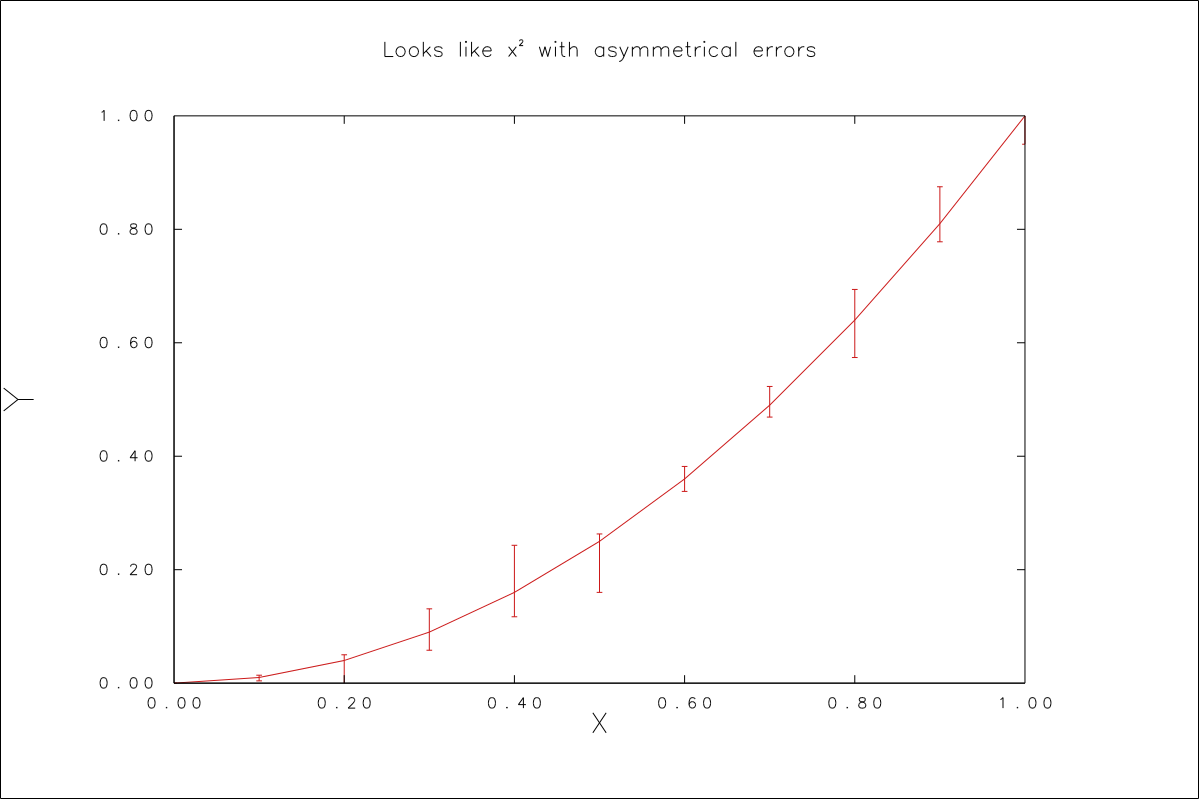
\includegraphics[width=\maxwidth]{../../temp/gr17001.eps}
  \caption{}
  \label{fig:gr17001}
\end{figure}

\newpara
Note that the column specified as the 3rd argument to \texttt{READ} is
the delta from the 2nd argument column value to the \emph{upper} limit
of the error bar, and the column specified as the 4th argument is the
(negative) delta to the \emph{lower} limit of the error bar.

\newpara
It is easy to plot points on top of this. This might be useful when the
points are derived from real measurements and a curve has been fitted to
these measurements. As an example of this, we take the point Y
coordinates from the 5th column of \texttt{DAEG3} using this script:

\begin{lstlisting}
# READ AN X,Y,EU,EL DATA FILE AND PLOT THE CONTENTS
#
RESET
GRAPHMODE ON
#
# --- READ THE DATA FILE, FIRST 3 COLUMNS. THIS ONE USES COMMAS.
ASYMYERRORS YES
GET DAEG3
READ DAEG3 1 2 3 4
#
# --- DRAW THE GRAPH
CSG ANNOT
COL 0 0 0
CSG TEXT
COL 0 0 0
CSG GEN
COL 0.8 0.1 0.1
TITLE "*LX*+2$+ WITH ASYMMETRICAL ERRORS AND POINTS"
XLABEL "X"
YLABEL "Y"
XYLINE
#
# --- PLOT POINTS
XYSAME
ANNOT OFF
CSG GEN
COL 0 0 1
SYMHT 0.04
READ DAEG3 1 5
XYPOINT
#
OUTLINE DEV
\end{lstlisting}

\newpara
This results in Figure~\ref{fig:gr18001}.

\begin{figure}
  \centering
  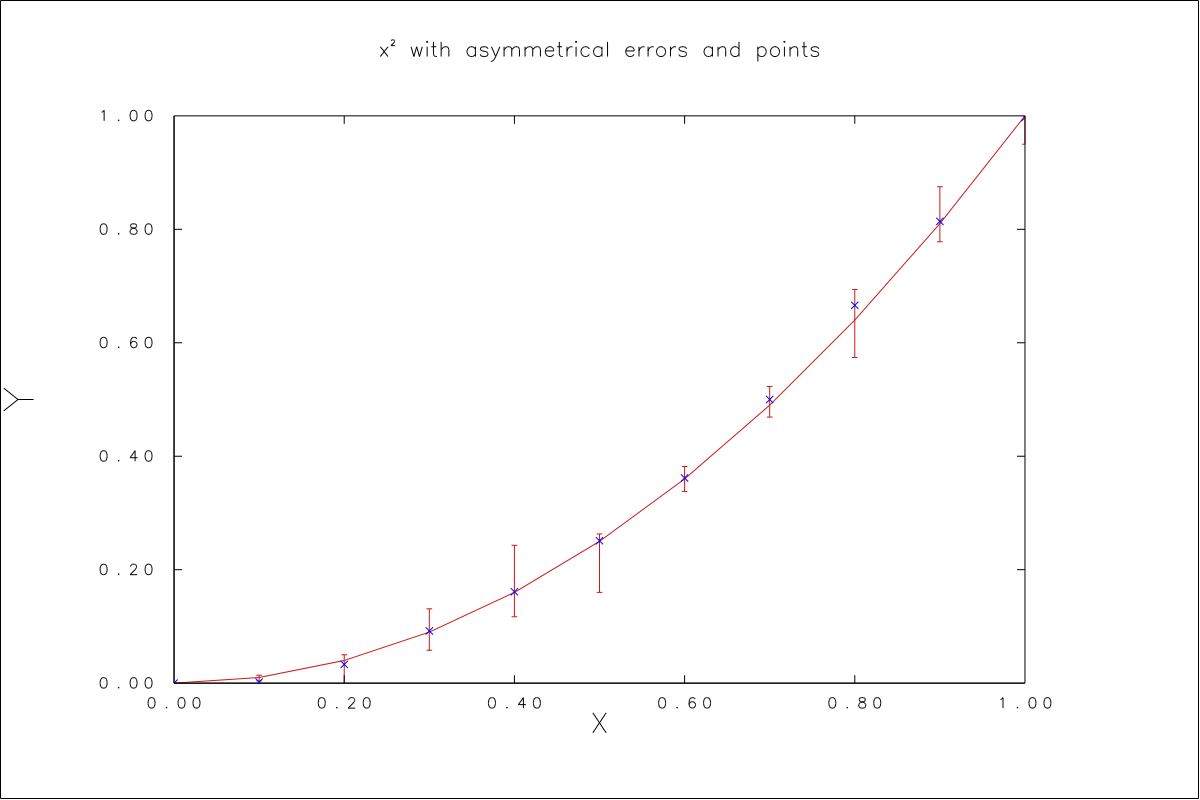
\includegraphics[width=\maxwidth]{../../temp/gr18001.eps}
  \caption{gr18001}
  \label{fig:gr18001}
\end{figure}


\subsection{Data with symmetric uncertainties in Y and X}\label{data-with-symmetric-uncertainties-in-y-and-x}
\newpara
It is also easy to plot data with uncertainty estimates in both axes
(see Figure~\ref{fig:gr1x001}).
This requires the same 4 data columns as used above, but with the
command:

\begin{lstlisting}
ASYMYERRORS NO
\end{lstlisting}

\newpara
Note that this \emph{must} appear \emph{before} the \texttt{READ}
command, as it causes data to be rearranged internally immediately after
it is read. In this case, the 3rd column is interpreted as symmetric Y
error and the 4th as symmetric X error.

\begin{figure}
  \centering
  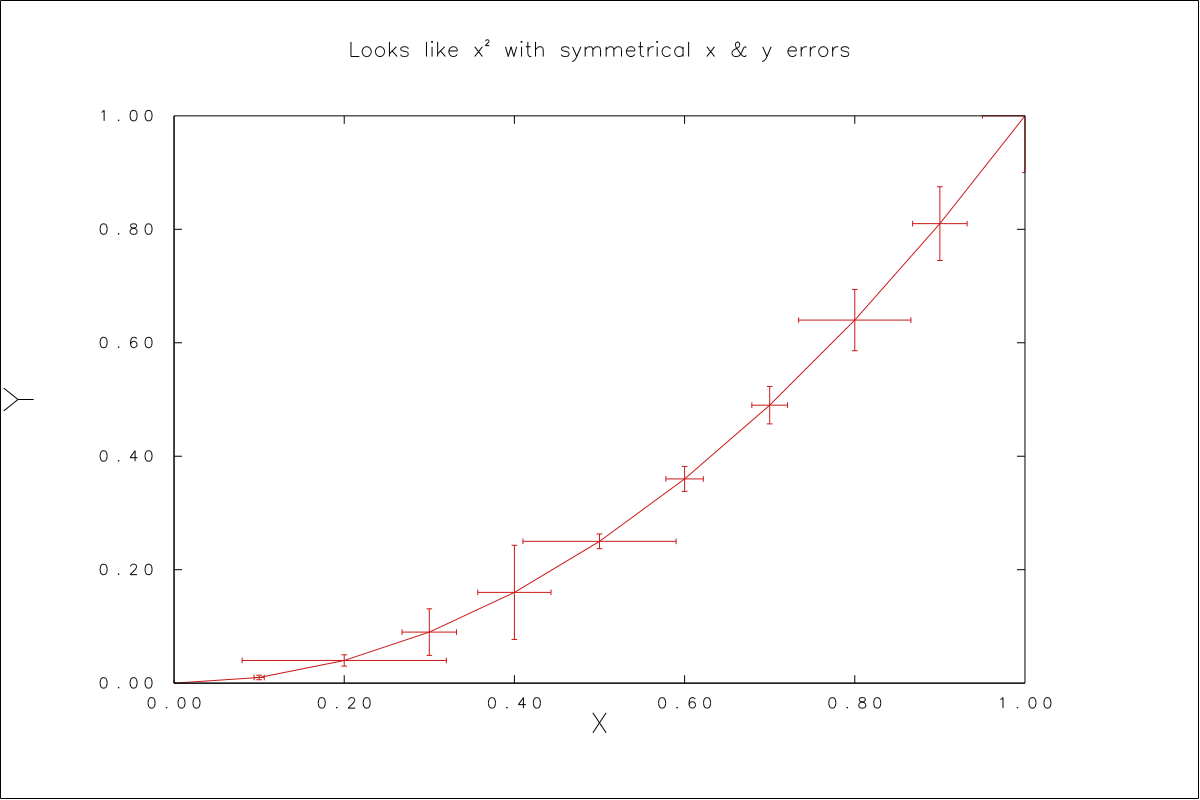
\includegraphics[width=\maxwidth]{../../temp/gr1x001.eps}
  \caption{Y and X error bars}
  \label{fig:gr1x001}
\end{figure}


\subsection{Interpolating the data points}\label{interpolating-the-data-points}
\newpara
The supplied data can be interpolated for the purposes of plotting
``smooth'' curves through, rather than straight lines between, the
supplied data. This is generally frowned upon in science, but
\textbf{GPLOT/DIMFILM} can do it!

\newpara
In addition to \texttt{LINEAR} interpolation (which is usually
pointless, as the appearance of the graph does not change), a cubic (3rd
order) or quintic (5th order) polynomial can be drawn through the data
points. At least 3 points must be supplied for cubic, and 5 for quintic,
interpolation. The data must be sorted in X. The number of points to be
found between each supplied point must be specified. If the data is not
reasonably ``well behaved'', there can be numerical issues.

\newpara
To demonstrate this capability, Figure~\ref{fig:gr1i001} shows a very simple example.

\begin{figure}
  \centering
  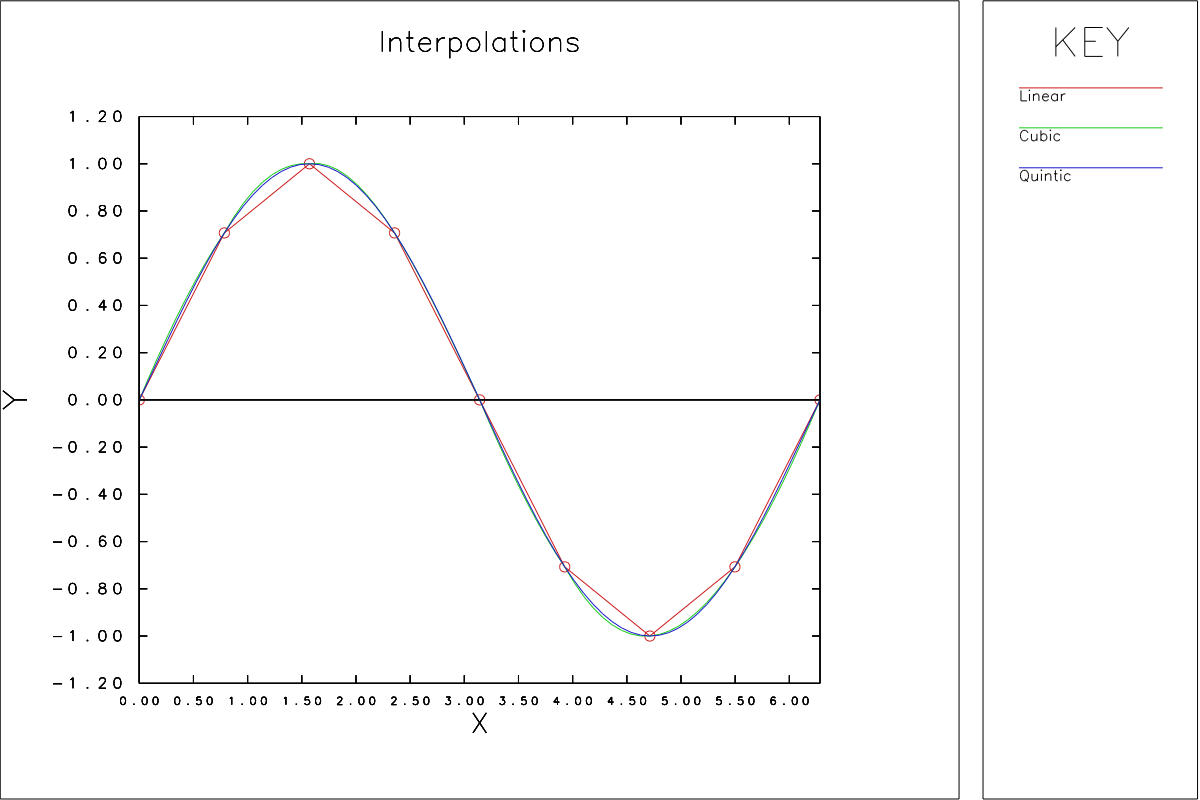
\includegraphics[width=\maxwidth]{../../temp/gr1i001.eps}
  \caption{Smooth interpolated curves through data points}
  \label{fig:gr1i001}
\end{figure}

\newpara
This is created by the following script:

\begin{lstlisting}
# INTERPOLATION
#
RESET
GRAPHMODE ON
#
# --- SOME DATA - VERY UNDERSAMPLED SIN(X)
READ HERE 1 2
0.00000  0.00000
0.78540  0.70711
1.57080  1.00000
2.35619  0.70711
3.14159  0.00000
3.92699 -0.70711
4.71239 -1.00000
5.49779 -0.70711
6.28319  0.00000
EOF
#
# --- SETUP THE GRAPH
USEKEY
CSG ANNOT
COL 0 0 0
CSG TEXT
COL 0 0 0
CSG GEN
COL 0.8 0.1 0.1
YRANGE -1.2 1.2
TITLE "I*LNTERPOLATIONS"
XLABEL "X"
YLABEL "Y"
#
# --- LINEAR INTERPOLATION, 9 INTERMEDIATES.
INTERPOLATE LINEAR 9
XYLINE
ADDKEY "L*LINEAR"
#
# --- POINTS BEING INTERPOLATED.
XYSAME
MARKER 20
XYPOINT
#
# --- CUBIC
COL 0.1 0.8 0.1
INTERPOLATE CUBIC 9
XYLINE
ADDKEY "C*LUBIC"
#
# --- QUINTIC
COL 0.1 0.1 0.8
INTERPOLATE QUINTIC 9
XYLINE
ADDKEY "Q*LUINTIC"
#
# --- FINISH THE GRAPH
KEYS
\end{lstlisting}


\subsection{Log Linear Plots}\label{log-linear-plots}
\newpara
It is possible to use a logarithmic Y axis and linear X axis. An example
of this is shown in Figure~\ref{fig:gr20001}.

\begin{figure}
  \centering
  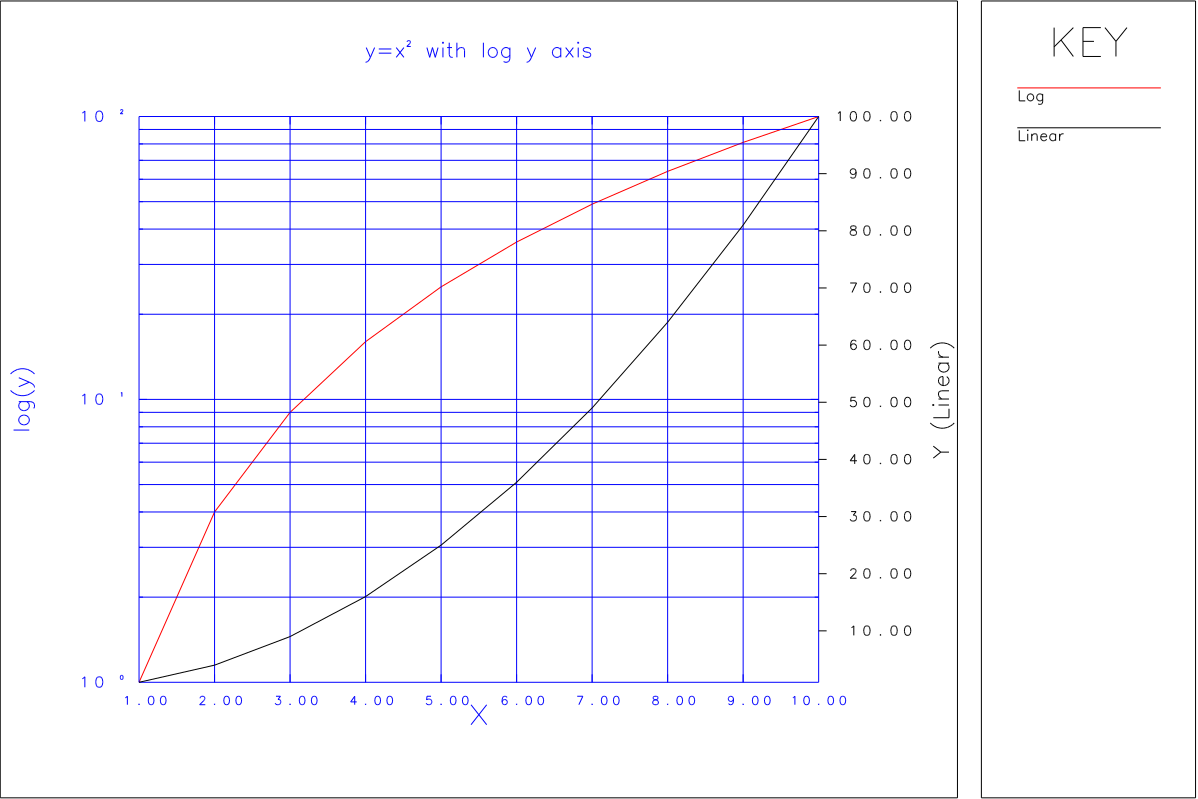
\includegraphics[width=\maxwidth]{../../temp/gr20001.eps}
  \caption{Log Y, linear X, $y=x^2$}
  \label{fig:gr20001}
\end{figure}

\newpara
Well, if we were hoping for a straight line with log Y for this
function, we are going to be disappointed! Here is the script fot this:

\begin{lstlisting}
# LOG Y AXIS
#
RESET
GRAPHMODE ON
CSG ANNOT
COL 0 0 1
CSG TEXT
COL 0 0 1
#
# --- SQUARES OF SOME NUMBERS.
READ HERE 1 2
1 1
2 4
3 9
4 16
5 25
6 36
7 49
8 64
9 81
10 100
EOF
#
# --- WE WILL USE KEYS.
USEKEY
#
# --- PLOT IT WITH LOG Y AXIS
XLAB "*LX"
YLABEL "*LLOG(Y)"
TITLE "*LY=X*+2$+ WITH LOG Y AXIS"
GRID BOTH
YLOG
XYLINE
ADDKEY "L*LOG"
ANNOT OFF
#
# --- PLOT IT WITH LINEAR Y AXIS, VALUES ON RIGHT
CSG ALL
COLOUR 0 0 0
RIGHTANNOT ON
RYLABEL "Y (L*LINEAR)"
YLIN
XYL
ADDKEY "L*LINEAR"
#
# --- DRAW LEGEND.
KEYS
#
# OUTLINE DEV
\end{lstlisting}

\newpara
Let's try a power function instead (Figure~\ref{fig:gr2a001}).

\begin{figure}
  \centering
  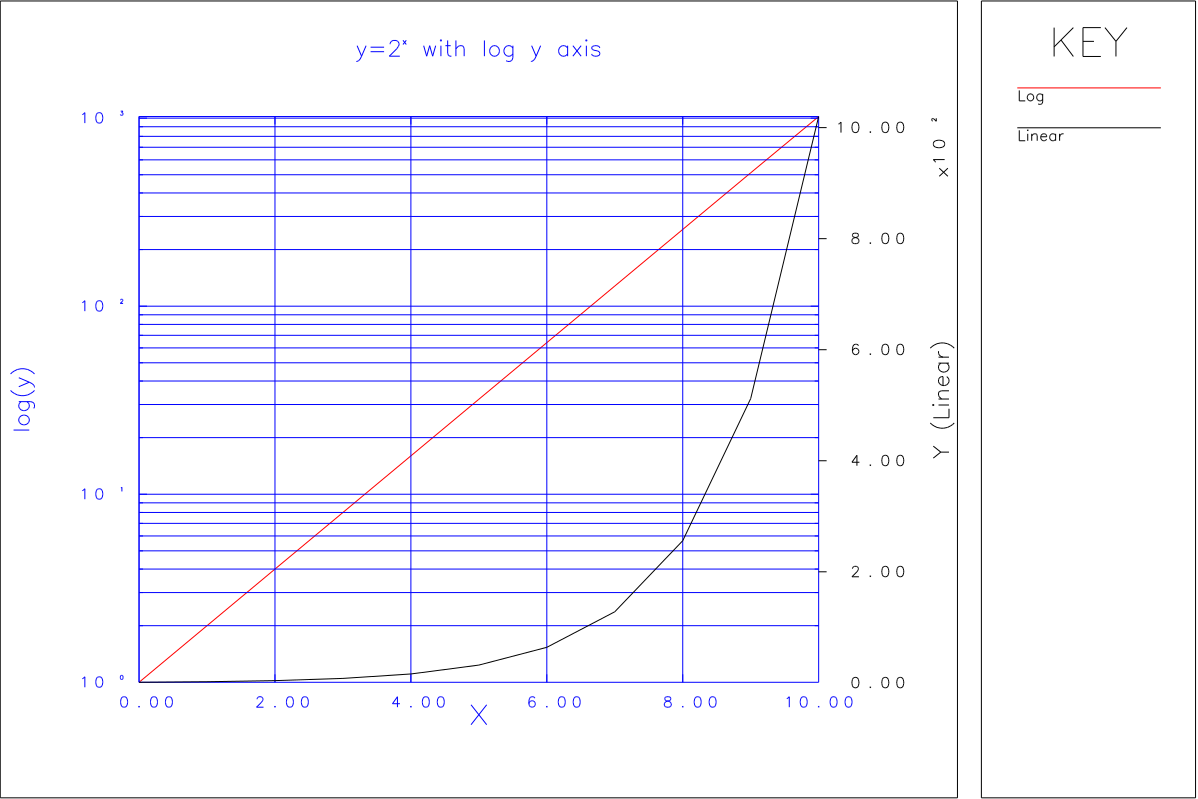
\includegraphics[width=\maxwidth]{../../temp/gr2a001.eps}
  \caption{Log Y, linear X, $y=2^x$}
  \label{fig:gr2a001}
\end{figure}

\newpara
Ah hah! This time we are in luck -- a straight line using a log-linear
plot!

\subsection{Log Log Plots}\label{log-log-plots}
\newpara
It is also easy to plot data with both log Y and log X axes. This script
will do that with the same data as shown in the first log-linear plot
(but with the values scaled up to see what happens):

\begin{lstlisting}
# LOG X AND Y AXIS
#
RESET
GRAPHMODE ON
#
CSG ANNOT
COL 0 0 1
CSG TEXT
COL 0 0 1
#
# --- SQUARES OF SOME NUMBERS.
READ HERE 1 2
1.0E7 1
2.0E7 4
3.0E7 9
4.0E7 16
5.0E7 25
6.0E7 36
7.0E7 49
8.0E7 64
9.0E7 81
1.0E8 100
2.0E8 400
3.0E8 900
4.0E8 1600
5.0E8 2500
6.0E8 3600
7.0E8 4900
8.0E8 6400
9.0E8 8100
1.0E9 10000
EOF
#
# --- WE WILL USE KEYS.
USEKEY
#
# --- PLOT IT WITH LOG X AND Y AXES
XLAB "*LLOG(X)"
YLABEL "*LLOG(Y)"
TITLE "*LY=(*,X$,10*+7$+$.)*O*+2$+$* WITH LOG X AND Y AXES"
GRID BOTH
XLOG
YLOG
XYLINE
ADDKEY "L*LOG"
#
# --- PLOT IT WITH LINEAR Y AXIS, VALUES ON RIGHT
ANNOT OFF
CSG ALL
COLOUR 0 0 0
RIGHTANNOT ON
RYLABEL "Y (L*LINEAR)"
YLIN
XYL
ADDKEY "L*LINEAR"
#
# --- DRAW LEGEND.
KEYS
\end{lstlisting}

\begin{figure}
  \centering
  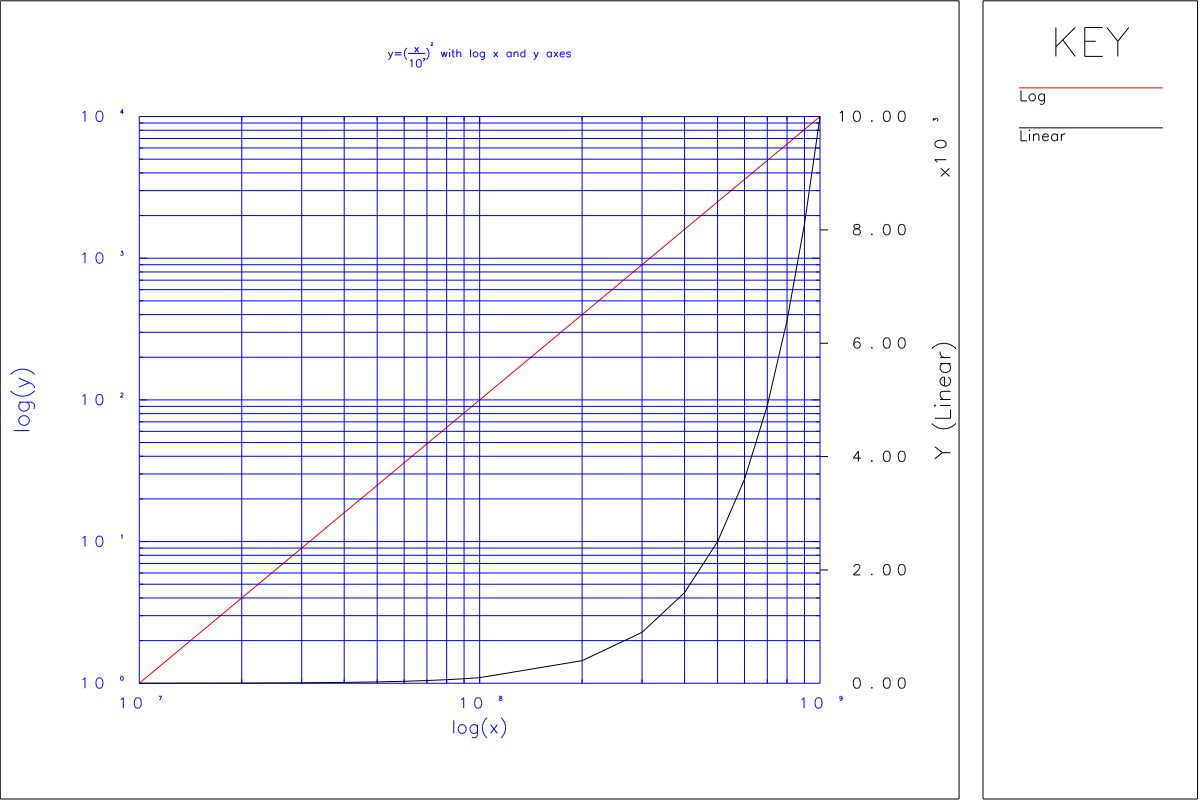
\includegraphics[width=\maxwidth]{../../temp/gr21001.eps}
  \caption{$y=\left(\frac{x}{10^7}\right)^2$}
  \label{fig:gr21001}
\end{figure}

\newpara
And we now have a straight line on the log-log plot for this function,
as shown in Figure~\ref{fig:gr21001}.

\newpara
Note that one of the main reasons people plot experimental data with
log-linear or log-log axes is in the hope of seeing something like a
straight line when they do so, which gives them a clue to the form of a
mathematical model which might ``explain'' the experimental data (or, at
least, approximate it).

\subsection{Histograms and multiple plots in one figure}\label{histograms-and-multiple-plots-in-one-figure}
\newpara
Histograms are another common type of plot and \textbf{GPLOT} can draw them in
various styles. There are no facilities for binning raw data so that
histograms can be drawn, however. Other software must prepare counts of
data points that fall into bins of specified ranges. All \textbf{GPLOT} deals
with are the counts and bin numbers for each count.

\newpara
As a minimal example, here is a single column of counts that can be
represented by a histogram (file \texttt{DAEG4}):

\begin{lstlisting}
100
123
90
20
10
1
200
233
129
43
77
6
2
9
64
99
12
18
111
87
\end{lstlisting}

\newpara
The following script draws histogram plots of this data in four
different styles:

\begin{lstlisting}
# READ A COUNTS ONLY DATA FILE AND MAKE HISTOGRAMS.
#
RESET
#
# --- READ THE DATA FILE, FIRST COLUMN ONLY.
GET DAEG4
READ DAEG4 0 1
#
# --- SET COLOURS
CSG ANNOT
COL 0 0 0
CSG TEXT
COL 0 0 0
CSG GEN
COL 0.8 0.1 0.1
#
# --- SET THE AXIS RANGES AND USE INT LABELS.
XRANGE -1 20
YRANGE 0 240
AXCUT NO
INTVALUES BOTH
#
# --- SET AXIS LABELS.
XLABEL "C*LLASS NUMBER"
YLABEL "C*LOUNT"
#
# --- ABUT STYLE IN BOTTOM LEFT.
PANE 0 0.5 0 0.5
HISTSTYLE ABUT
TITLE "C*LOUNTS HISTOGRAM (ABUTTING BARS)"
XYHIST
OUTLINE PANE
#
# --- SHADED ABUT STYLE IN BOTTOM RIGHT.
PANE 0.5 1 0 0.5
HISTSTYLE ABUT+SHADE
TITLE "C*LOUNTS HISTOGRAM (ABUTTING SHADED BARS)"
XYHIST
OUTLINE PANE
#
# --- SPECIFIED WIDTH BARS IN TOP LEFT.
PANE 0 0.5 0.5 1
HISTSTYLE WIDE 0.25
TITLE "C*LOUNTS HISTOGRAM (SPECIFIED WIDTH BARS)"
XYHIST
OUTLINE PANE
#
# --- THIN LINES IN TOP RIGHT.
PANE 0.5 1 0.5 1
HISTSTYLE LINES
TITLE "C*LOUNTS HISTOGRAM (IMPULSES)"
XYHIST
OUTLINE PANE
#
OUTLINE DEV
\end{lstlisting}

\newpara
The result is shown in Figure~\ref{fig:gr22001}.

\begin{figure}
  \centering
  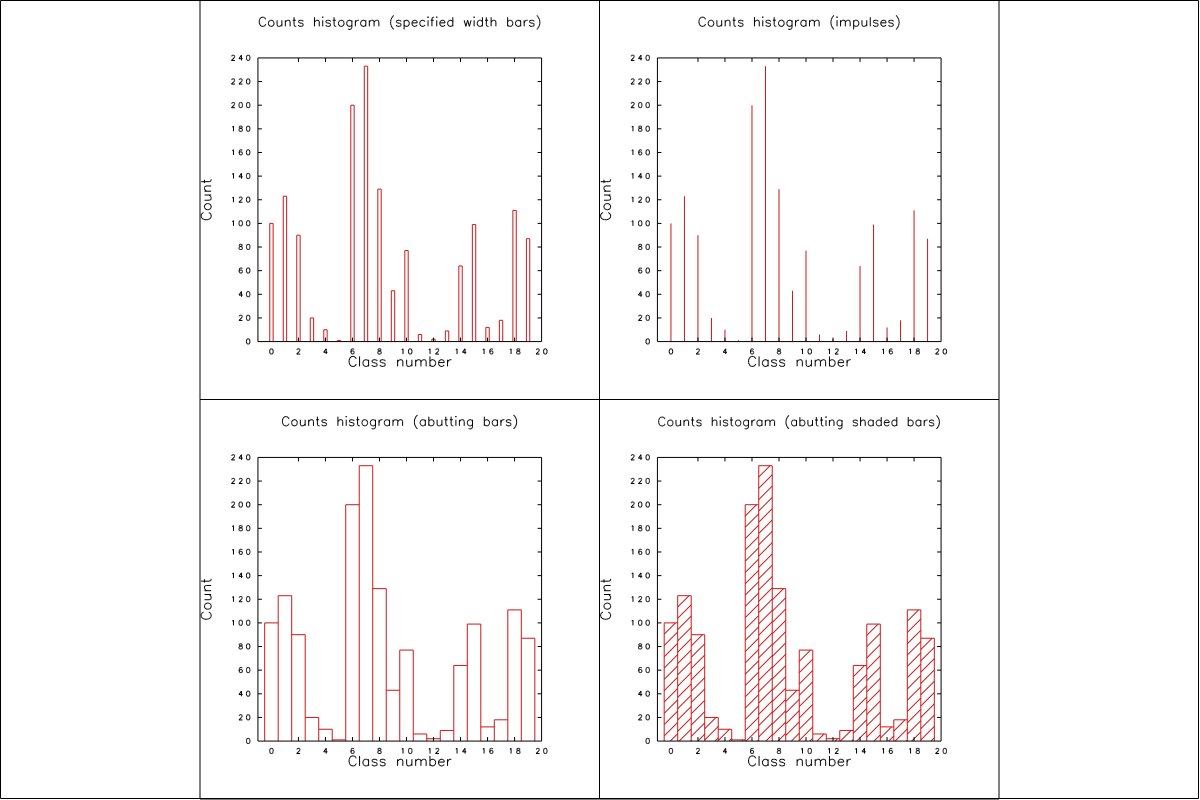
\includegraphics[width=\maxwidth]{../../temp/gr22001.eps}
  \caption{Histograms and sub-figures using \texttt{PANE} explicitly}
  \label{fig:gr22001}
\end{figure}

\newpara
In addition to showing how to draw histogram plots, this example shows a
number of other new features.

\begin{itemize}
\item
  We explicitly specify X and Y axis ranges rather than letting the
  software choose. This is done with the \texttt{XRANGE} and
  \texttt{YRANGE} commands.
\item
  We prevent lines being drawn for the axes -- vertical and horizontal
  lines that pass through (0,0) (or another point specified with
  \texttt{AXCUT}) -- by using: \texttt{AXCUT\ NO}
\item
  We try to use integers for the axis values instead of floating point
  numbers using \texttt{INTVALUES\ BOTH}. This option can be requested
  for X, Y, both or neither axis. It may not always be honoured, as it
  will be impossible for many axis ranges. But in this case, it is a
  reasonable request and it works.
\end{itemize}

\newpara
The most obvious new feature, though, is that the four plots showing the
different histogram drawing styles appear in a single ``figure''.

\newpara
This can be done easily with \textbf{DIMFILM}, as graphs are plotted inside any
specified ``pane'' (see above), so all you have to do is use
\texttt{PANE} appropriately.

\newpara
Actually, though, that needs some (trivial) manual calculation, but it
may also need to account for the device aspect ratio if the output
canvas is to be filled. To further simplify creating multiple plots in a
single ``figure'', \textbf{GPLOT} has the \texttt{SUBFIGGRID} command (which can
be abbreviated, fortunately). This lets you specify a rectangular
arrangement of ``sub-figures'' and the current sub-figure to be drawn
(before any plotting commands) and calculates an appropriate pane for
you, accounting for the device's aspect ratio (if \texttt{GRAPHMODE\ ON}
has been used). It also lets you ``shrink'' the figure, so there is some
white space between it and its neighbours.

\newpara
An example of using this is shown in Figure~\ref{fig:gr29001}.

\begin{figure}
  \centering
  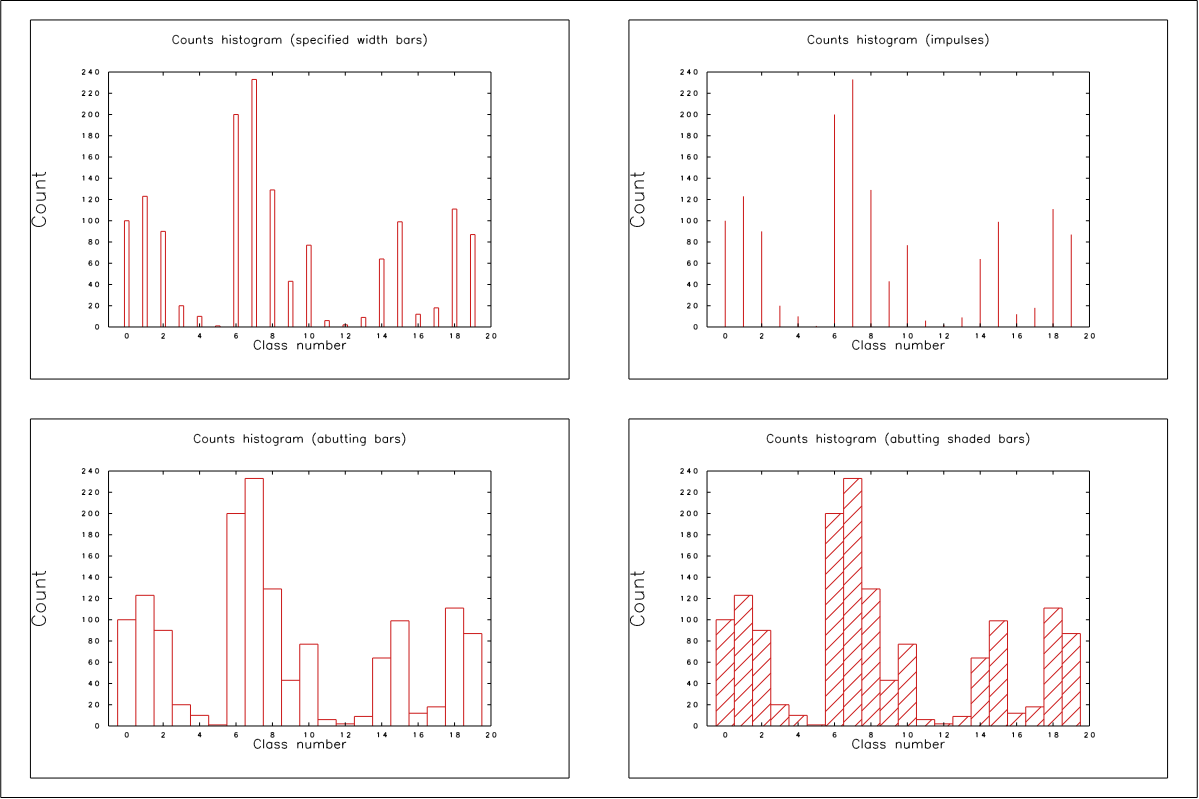
\includegraphics[width=\maxwidth]{../../temp/gr29001.eps}
  \caption{Histograms and sub-figures using \texttt{SUBFIGGRID}}
  \label{fig:gr29001}
\end{figure}


%% \begin{figure}
%%  \centering
%%  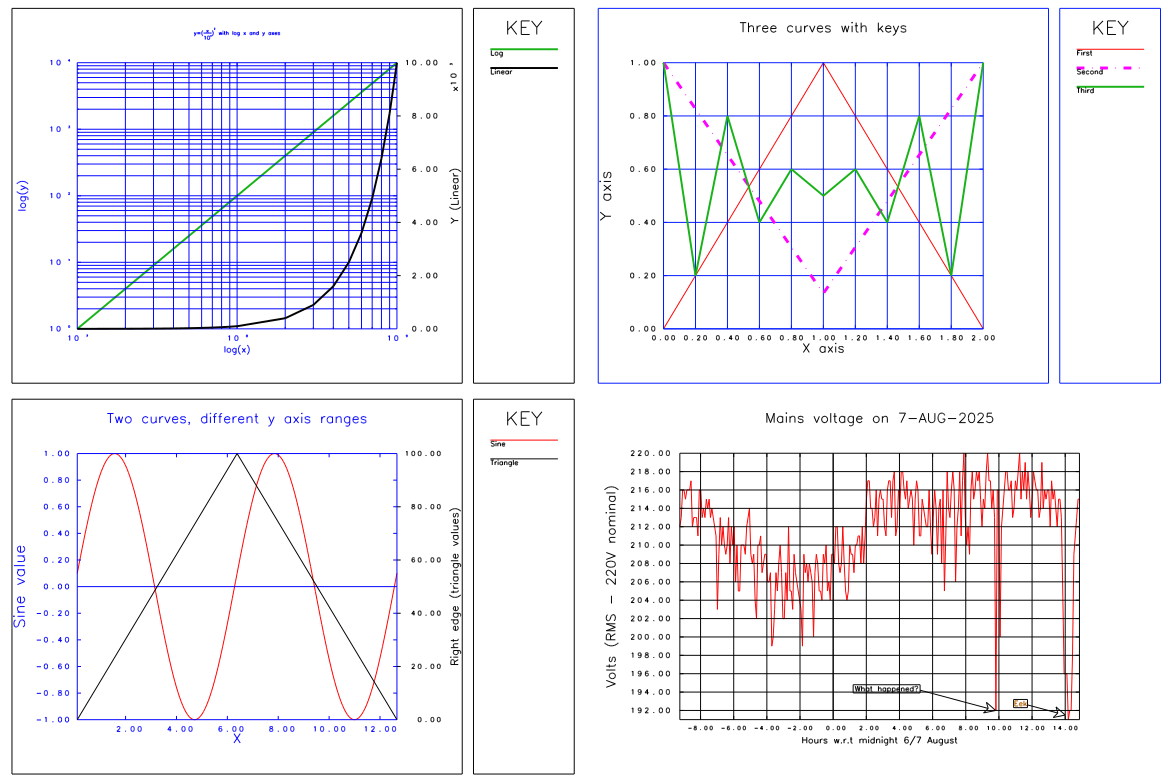
\includegraphics[width=\maxwidth]{../../temp/gr28001.eps}
%%  \caption{gr28001}
%%  \label{fig:gr28001}
%% \end{figure}

\newpara
The script for that is very similar to the one above, but with these
changes:

\begin{lstlisting}
# READ A COUNTS ONLY DATA FILE AND MAKE HISTOGRAMS.
#
RESET
GRAPHMODE ON
...
#
# --- ABUT STYLE IN BOTTOM LEFT.
SUBFIG 2 2 1 1 0.95
HISTSTYLE ABUT
...
#
# --- SHADED ABUT STYLE IN BOTTOM RIGHT.
SUBFIG 2 2 2 1 0.95
HISTSTYLE ABUT+SHADE
...
#
# --- SPECIFIED WIDTH BARS IN TOP LEFT.
SUBFIG 2 2 1 2 0.95
HISTSTYLE WIDE 0.25
...
#
# --- THIN LINES IN TOP RIGHT.
SUBFIG 2 2 2 2 0.95
HISTSTYLE LINES
...
#
OUTLINE DEV
\end{lstlisting}


\subsection{Multiple plots with keys in one figure.}\label{multiple-plots-with-keys-in-one-figure.}
\newpara
The ``sub-figures'' feature also works with graphs with keys (some
juggling of panes is involved internally). An example of this is
Figure~\ref{fig:gr27001}.

\begin{figure}
  \centering
  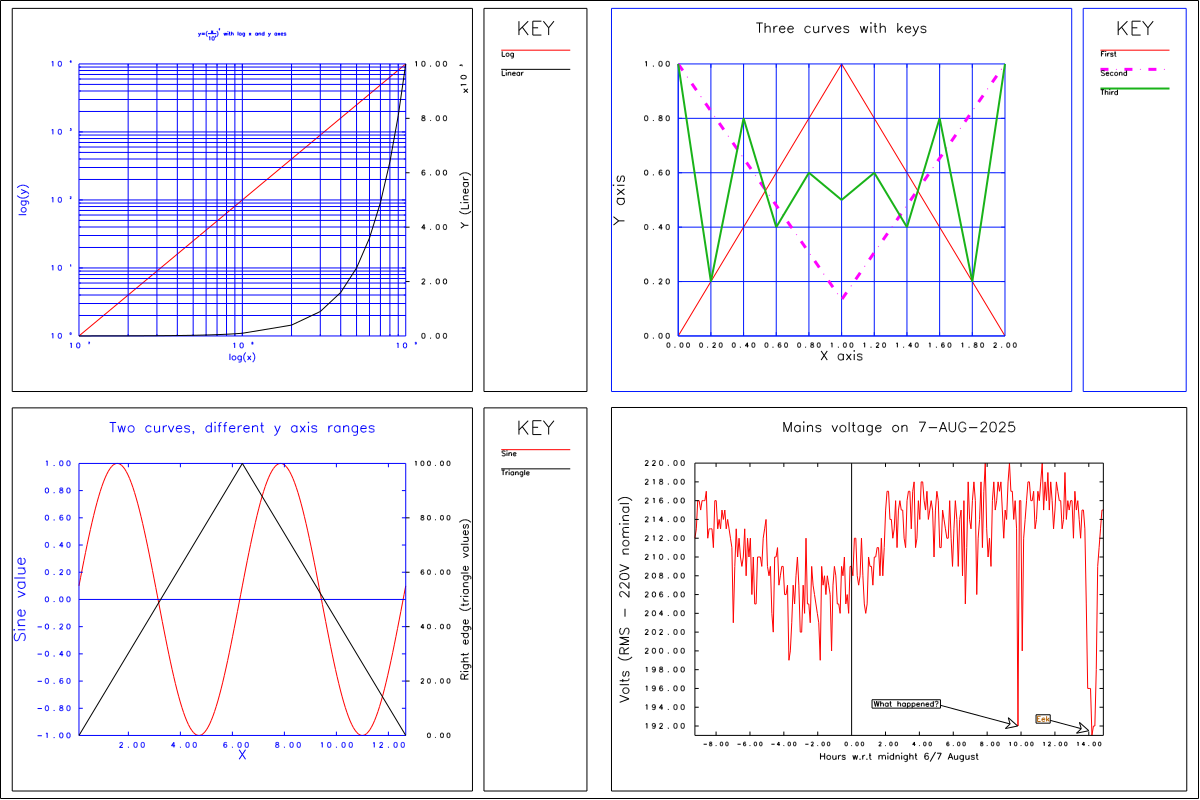
\includegraphics[width=\maxwidth]{../../temp/gr27001.eps}
  \caption{Different plots, some with keys, in one figure}
  \label{fig:gr27001}
\end{figure}

\newpara
This redraws four of the example plots shown above. Some minor changes
to the scripts that drew them were made (any \texttt{RESET},
\texttt{GRAPHMODE} or other commands that changed the bounds or pane
were removed). These modified versions are stored in the script files
\texttt{OBGF28A}, \texttt{OBGF28B}, \texttt{OBGF28C} and
\texttt{OBGF28D}. These are then ``called'' from a ``master'' script
file \texttt{OBGF28M} (obey files can be nested up to 5 levels deep):

\begin{lstlisting}
# FOUR DISPARATE PLOTS, ONE FIGURE.
#
#===========================
RESET
GRAPHMODE ON
# --- BOTTOM LEFT OF 4
SUBFIG 2 2 1 1 0.98
#
OBEY OBGF28A
#===========================
RESET
GRAPHMODE ON
# --- TOP RIGHT OF 4
SUBFIG 2 2 2 2 0.98
#
OBEY OBGF28B
#
# ========================
RESET
GRAPHMODE ON
# --- TOP LEFT OF 4
SUBFIG 2 2 1 2 0.98
#
OBEY OBGF28C
# ========================
# --- BOTTOM RIGHT OF 4
RESET
GRAPHMODE ON
SUBFIG 2 2 2 1 0.98
#
OBEY OBGF28D
OUTLINE PANE
#
OUTLINE DEV
\end{lstlisting}

\newpara
(Note that files will be stored on ``Unix-like'' systems with lower case
file names but may be referred to in upper case in \textbf{GPLOT} -- all file
names are converted internally to lower case by \textbf{GPLOT} on ``Unix'' before
being accessed. These names could appear in lower case -- as could all
commands -- and it would work)

\newpara
Please example the ``called'' scripts for more information.

\newpara
When generating a multi-plot ``figure'', you must keep the grid size
constant in the \texttt{SUBFIG} command (e.g.~\texttt{SUBFIG\ 2\ 2}) for
every sub-figure. This is probably obvious, but nothing can check for
this.

\newpara
Note the repetition of \texttt{RESET} and \texttt{GRAPHMODE\ ON} for
each sub-figure. Without this, the various colours and styles set in one
sub-figure script would be inherited by the next. These must occur
\emph{before} the \texttt{SUBFIG} command, so they cannot be left in the
script files.


\subsection{Using the RPN evaluator to plot simple functions}\label{using-the-rpn-evaluator-to-plot-simple-functions}

\newpara
\textbf{GPLOT} includes a feature for calculating function values rather than
reading them from files. This is the Reverse Polish Notation (RPN)
evaluator, which provides features very similar to those you would find
on classic HP calculators.

\newpara
One difference is that the RPN evaluator often operates on \emph{arrays}
rather than scalar values, in a way that might be familiar to people who
have used NumPy or an APL-like language, perhaps. But with RPN thrown in
for extra confusion!

\newpara
The evaluator has quite a few features beyond those needed for simple
function plotting, and its main limitation is perhaps that the
``program'' length is limited by the 80 character input line limit
(beyond which all input is truncated).

\newpara
A complete description of the available operators can be found in the
``cheat sheet'' below (which uses a notation familar to FORTH users) and
in the PDF format \textbf{GPLOT} manual. Here, we just give some examples as an
introduction.

\newpara
Admittedly, the RPN evaluator may not be all that easy to use (the
\texttt{DUMP} operator is helpful when debugging), but it opens up a lot
of possibilities.

\newpara
When dealing with data from files, \textbf{GPLOT} uses between 2 and 4 arrays to
store the data to be plotted. Two are used to store X and Y coordinates.
If symmetric error bars are to be plotted a third array is used to store
that, and asymmetric Y error bars or Y and X error bars use a fourth
array.

\newpara
The RPN evaluator treats these four arrays as the first four levels of a
stack. If \texttt{READ} is used, their contents will be overwritten by
the read data and the array length seen by the evaluator will be the
number of points read.

\newpara
To provide ``room'' for any but the simplest calculations, another 4
stack levels (arrays) are provided ``above'' to four used for data from
\texttt{READ}. (This can be configured with the \texttt{NSTACK}
command).

\newpara
It is possible to use the first two X and Y levels of the stack as
inputs to the evaluator. More often, though, the contents of the X array
are set to cover some range of values by the \texttt{ERANGE} command or
certain evaluator operators, and the evaluator sets the Y values in the
Y array. This is how it can fairly straightforwardly plot mathematical
functions.

\newpara
The evaluator ``cheat sheet'' below tries to show this stack of arrays
diagrammatically.

\newpara
As a first, very simple, example, let's compute ``y=x\^{}2''. In
previous examples the data has been precomputed and read from a file
(often a ``HERE'' file). This script generates the y values for a
defined range of x values and plots the result (left hand subfigure,
Figure~\ref{fig:gr30001}).

\begin{lstlisting}
RESET
GRAPHMODE ON
#
CSG ANNOT
COL 0 0 0
CSG TEXT
COL 0 0 0
#
ERANGE 1 1 100 100
EVAL X,2,**
#
XLABEL "X"
YLABEL "Y"
TITLE "X*+2"
GRID BOTH
XYLINE
#
OUTLINE DEV
\end{lstlisting}

\begin{figure}
  \centering
  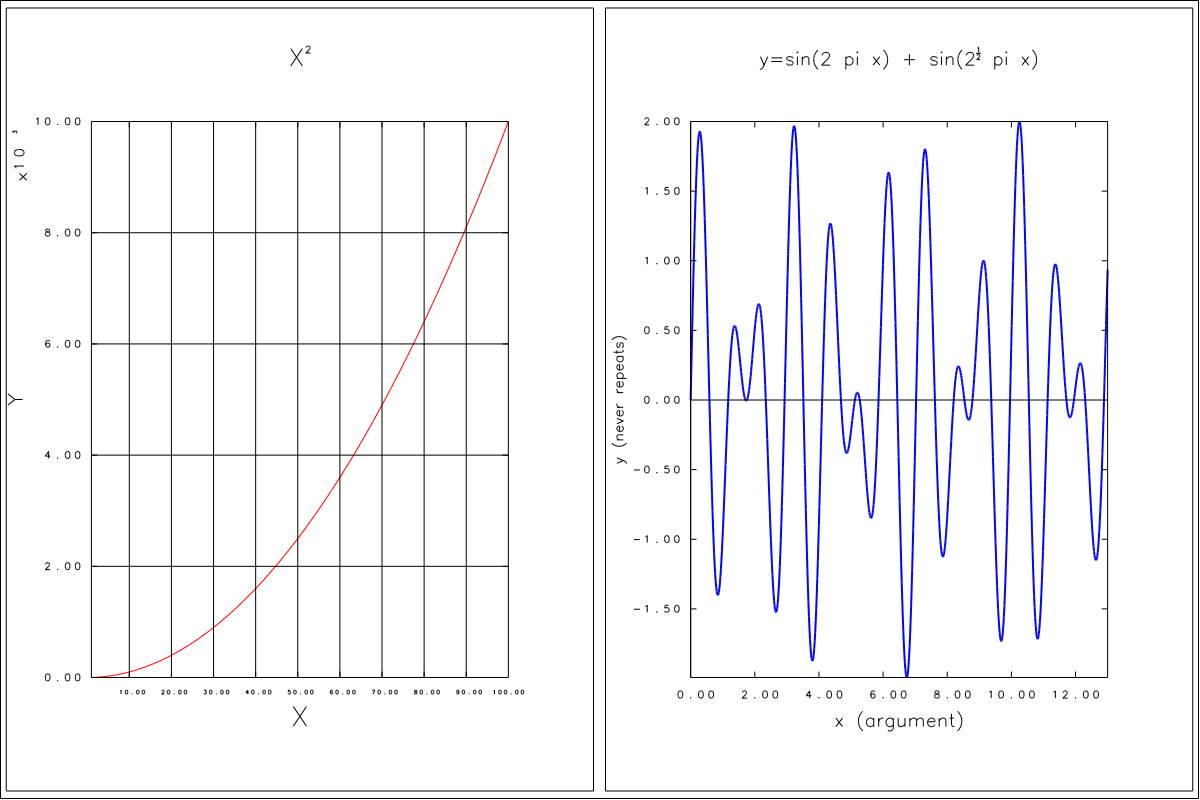
\includegraphics[width=\maxwidth]{../../temp/gr30001.eps}
  \caption{Graphs of functions calculated by the evaluator}
  \label{fig:gr30001}
\end{figure}

\newpara
The two commands that generate the data to be plotted are
\texttt{ERANGE} and \texttt{EVAL}. The \texttt{ERANGE} command defines a
range of x values for which the function is the be evaluated. In the
case given here, it is similar to the NumPy ``linspace'' function. The
first argument is the logarithm base, which, if 1, indicates we want to
sample a linear range. The next two values are the start and end x
values, and the final argument is the number of steps to take between
start and end. \texttt{ERANGE} puts its output in the X array, which is
also stack level 0.

\newpara
The RPN evaluator does not use the X array as a ``normal'' part of the
stack. It can be read via the \texttt{X} operator, which pushes its
contents on the stack. The X array can be written to by the
\texttt{SETX} operator. Otherwise, it is not accessed.

\newpara
The \texttt{EVAL} operator needs one argument (a second is optional)
which is an ``RPN string'' containing operators and operands for the
evaluator to, er, evaluate. It may be enclosed in double quotation
marks.

\newpara
Whatever the evaluator leaves in the stack level 1 or Y array can be
plotted against the X array contents using \texttt{XYLINE} or the other
graphing commands.

\newpara
To make the evaluator more useful, there are 9 ``procedure registers''
which can contain ``RPN strings''. These can be executed by the
evalautor using the notation:

\begin{lstlisting}
EVAL @1
EVAL @1,@3
\end{lstlisting}

\newpara
which ``calls'' one or more procedure register contents (sequentially).
The contents of a ``procedure register'' can be set with the
\texttt{PROC} command. They can also be set with the \texttt{LOADPROC}
command, which looks for a named procedure in the file \texttt{GPLPROC}
and loads it into a specified ``procedure register'' if it is found.

\newpara
Note that the \textbf{GPLOT} evaluator does not actually do a ``call and return''
when it sees \texttt{EVAL\ @1}, etc. Instead, it uses string
substitution to replace \texttt{@1} with the string in procedure
register 1. It does this repeatedly, if necessary, until there are no
remaining \texttt{@n} sequences in the substituted string.

\newpara
There are also 9 \emph{scalar} ``memory'' registers, which can be set
with the \texttt{STO} command and recalled with \texttt{RCL}. Often,
parameters for procedures are put into these registers with \texttt{STO}
then accessed in the RPN with the \texttt{RCL} or (as an abbreviation)
\texttt{\#}.

\newpara
To make evaluating procedures with parameters more straightforward, the
optional second argument to \texttt{EVAL} is a comma separated list of
numeric values to \texttt{STO} into consecutive scalar registers
(starting with the 1st) before running the RPN string. For example,

\begin{lstlisting}
EVAL @1 "1,2,3,4"
\end{lstlisting}

\newpara
would put 1 in scalar register 1, 2 in register 2, and so on, then
``call'' the procedure in ``procedure register'' 1.

\newpara
Finally, there are 9 ``string registers'' which can be set with
arbitrary strings (maximum 80 characters) using the \texttt{STRING}
command. These can then be used in an RPN procedure for plotting text.

\newpara
Returning to plotting simple functions, this script graphs a slightly
more complex function:

\begin{lstlisting}
CSG ALL
COL 0 0 0
WIDTH 1
CSG GENERAL
COL 0 0 1
WIDTH 2
#
ERANGE 1 0 13 801
EVAL X,TWPI,*,SIN,X,PI,2,SQRT,*,*,SIN,+
#
XLABEL "*LX (ARGUMENT)"
YLABEL "*LY (NEVER REPEATS)"
TITLE "*LY=SIN(2 PI X) + SIN(2*+*,1$,2$.$+ PI X)"
XYL
\end{lstlisting}

\newpara
This is plotted in the righthand sub-figure of Figure~\ref{fig:gr30001}.
This function is
mathematically interesting, as it never repeats (i.e.~its period is
infinite). This will not be the case when it is plotted on a digital
computer, though, as all numbers on such machines are rational, but the
period will be enormous.


\subsection{General drawing - Part 1: Basic functions}\label{general-drawing---part-1-basic-functions}

\newpara
\textbf{DIMFILM} provides some basic drawing capabilities apart from its
extensive graph plotting functionality. Graph plotting is based on these
lower level capabilities, as you would expect.

\newpara
There is a simple but sound foundation for general drawing with the
\texttt{BOUNDS} command, which establishes a user defined coordinate
system, the \texttt{PANE} command, which sets up a rectangle in bounds
coordinates outside of which no drawing will occur (a ``clip to inside''
region) and the \texttt{BLANK} command, which sets a rectangle inside of
which no drawing will occur (a ``clip to outside'' region). These
commands map directly to \textbf{DIMFILM} subroutines.

\newpara
For convenience, \textbf{GPLOT} adds a \texttt{CANVAS} command, which just sets
the bounds and the pane to the same coordinate ranges.

\newpara
All general purpose drawing uses the coordinates established by
\texttt{BOUNDS}. If no explicit \texttt{BOUNDS} command is given, this
defaults to 0 to 1 by 0 to 1, which will be a square region, centered in
the output device drawable rectangle. As noted above, to use the full
area of the output device, the aspect ratio of the bounds must match the
aspect ratio of the device. This can be done automatically for graph
plotting applications using \texttt{GRAPHMODE\ ON}, but you will
generally want to choose your own coordinate ranges for general drawing,
often bearing the device aspect ratio in mind when doing do.

\newpara
The low level drawing operations available are \texttt{MOVE} to move the
``current position'' to a specified coordinate, \texttt{DRAW} to draw
from the current postion to a new position (which becomes the current
position) in a straight line, \texttt{CIRCLE} which draw a circle of a
given radius at a given position, \texttt{ARC} which draws a segment of
a circle, and \texttt{RECT} which draws a rectangle.

\newpara
Two \textbf{GPLOT} commands build slightly on this: \texttt{CRECT} draws a
rectangle centered on a given location and \texttt{PATH} uses the
contents of the X and Y arrays to draw a polyline. \textbf{GPLOT/DIMFILM} does
not support the drawing of any kinds of smooth curves for general
drawing purposes (\texttt{INTERPOLATE} can interpolate smooth curves
between data points for graph plotting, but this can't be used for
general drawing).

\newpara
\textbf{DIMFILM} has very limited geometric transformation support and \textbf{GPLOT} does
not provide access to this. \textbf{GPLOT} does provide a more comprehensive
geometric transformation capability through its RPN evaluator, though.

\newpara
While these graphics facilities are fairly basic, there is also a rather
comprehensive set of facilities for drawing text using vector fonts.
These are accessed through the \texttt{TEXT} and \texttt{CTEXT}
commands, with various properties set by the \texttt{SYMHT},
\texttt{SYMANG} and \texttt{FONT} commands. The fonts are specific to
\textbf{DIMFILM} (there is no way to use any ``system fonts''!) and are, in this
implementation, some of the Hershey fonts. The available fonts can be
listed with the \texttt{LISTFONT} command.

\newpara
Special ``marker'' characters can also be drawn using the
\texttt{MARKER} command with the optional 2nd argument set to
\texttt{YES}.

\newpara
The text output facility allows ``markup'' to be included in the string
to draw, and this extends to sub-scripts, super-scripts, and fractions,
which can be nested to two levels. Mathematical notation can, to a
useful degree, be accommodated by this. Although we have high quality
font drawing everywhere now (and for the last few decades), when \textbf{DIMFILM}
was first released (1973), this was cutting edge. Mathematical notation
is still not readily expressible everywhere it might be useful even
today, in fact.

\newpara
An example which shows most of the basic drawing operations in action
is Figure~\ref{fig:gd01001}.

\begin{figure}
  \centering
  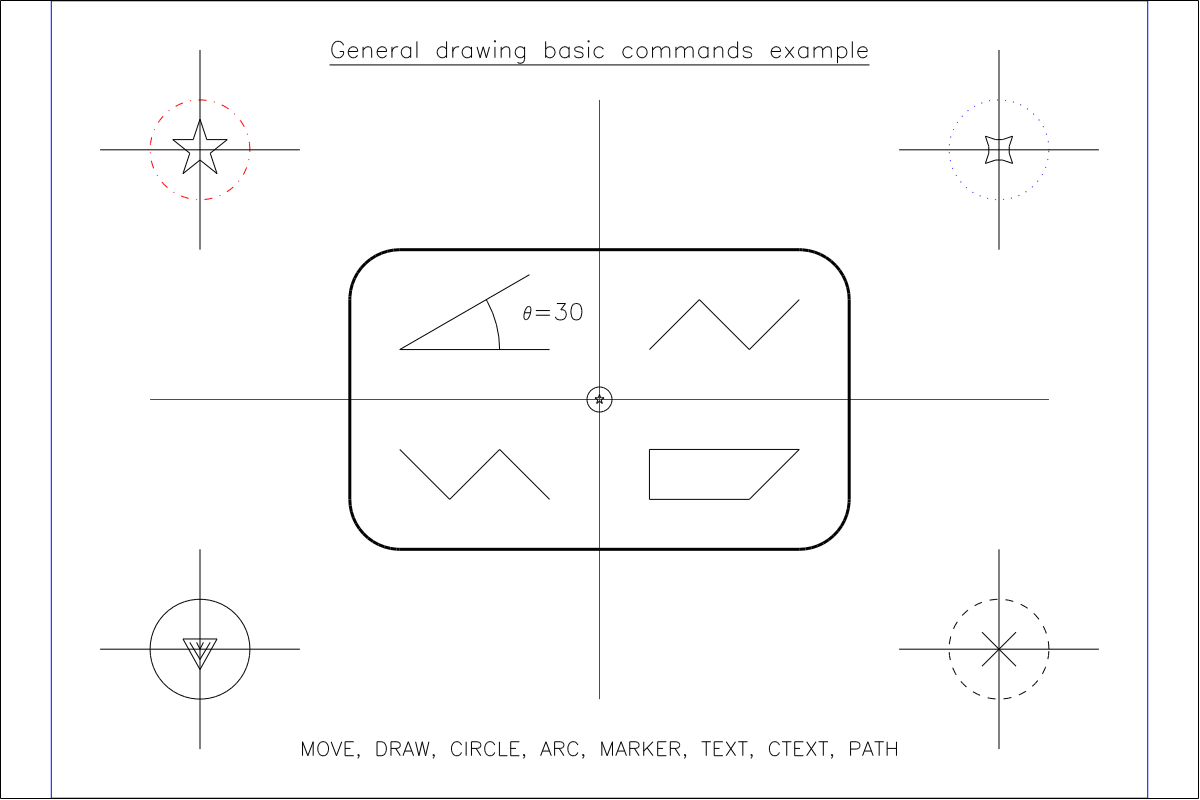
\includegraphics[width=\maxwidth]{../../temp/gd01001.eps}
  \caption{Basic drawing functions}
  \label{fig:gd01001}
\end{figure}

\newpara
The script for this is a little long, but may be worth presenting in
full:

\begin{lstlisting}
RESET
CANVAS 0 22 0 16
#
CSG TEXT
COL 0 0 0
CSG GEN
COL 0 0 0
#
# DRAW CIRCLES
CIRCLE 3 3 1
STYLE DASH
CIRCLE 19 3 1
STYLE DOT
COL 0 0 1
CIRCLE 19 13 1
STYLE DASHDOT
COL 1 0 0
CIRCLE 3 13 1
STYLE SOLID
COL 0 0 0
#
# DRAW ANGLE
MOVE 7 9
DRAW 10 9
MOVE 7 9
DRAW 9.5981 10.5
ARC 7 9 2 0 30
MOVE 9.45 9.5
SYMHT 0.5
TEXT "*:83=30"
#
# DRAW CENTER CROSS + MARKERS
COL 1 0 0
MOVE 2 8
DRAW 20 8
MOVE 11 2
DRAW 11 14
MOVE 11 8
COL 0 0 0
MARKER 9 Y
MARKER 23 Y
#
# DRAW CIRCLE CROSSES AND MARKERS
MOVE 1 13
DRAW 5 13
MOVE 3 11
DRAW 3 15
SYMHT 3
MOVE 3 13
MARKER 9 Y
#
MOVE 17 13
DRAW 21 13
MOVE 19 11
DRAW 19 15
MOVE 19 13
MARKER 24 Y
#
MOVE 1 3
DRAW 5 3
MOVE 3 1
DRAW 3 5
MOVE 3 3
MARKER 13 Y
#
MOVE 17 3
DRAW 21 3
MOVE 19 1
DRAW 19 5
MOVE 19 3
MARKER 3 Y
#
# DRAW ROUND CORNER RECTANGLE
WIDTH 3
ARC 7 6 1 180 270
ARC 15 6 1 270 360
ARC 7 10 1 90 180
ARC 15 10 1 0 90
MOVE 6 6
DRAW 6 10
MOVE 16 6
DRAW 16 10
MOVE 7 5
DRAW 15 5
MOVE 15 11
DRAW 7 11
WIDTH 1
#
# ODDITIES
MOVE 7 7
DRAW 8 6
DRAW 9 7
DRAW 10 6
#
MOVE 12 9
DRAW 13 10
DRAW 14 9
DRAW 15 10
#
READ HERE 1 2
12 6
14 6
15 7
12 7
EOF
PATH C
#
SYMHT 0.5
MOVE 11 15
CTEXT 0 "*=G*LENERAL DRAWING BASIC COMMANDS EXAMPLE$="
MOVE 11 1
CTEXT 12 "MOVE, DRAW, CIRCLE, ARC, MARKER, TEXT, CTEXT, PATH"
#
CSG GEN
COL 0 0 1
OUTLINE BOUNDS
OUTLINE DEV
\end{lstlisting}

\newpara
Most of this is likely to be self explanatory. The only points that may
be unclear are:

\begin{itemize}
\item
  The use of a ``special character'' from the symbol font (which is
  loaded with \texttt{MATH.SMALL} by default) to draw the ``theta''
  character. This is done by: \texttt{TEXT\ "*:83=30"} where the
  ``theta'' is selected by character number (83) using string markup.
  How do we know which character number to use? By looking at ``font
  tables'' which can be generated with one of the supplied script files
  (\texttt{obfont} for ``normal'' alphabets, \texttt{obsyms} for symbols
  and \texttt{obmarks} for markers). This is explained further in a
  later section (below).
\item
  The \texttt{MARKER} command, which will draw a specified marker (which
  is determined by a number) at the current position \emph{if} a second
  argument (\texttt{YES} - abbreviated, any case) is supplied. If only
  one argument is supplied, the \texttt{MARKER} command sets the marker
  number to use for points when plotting graphs.
\item
  Polyline paths can be drawn with the \texttt{PATH} command with
  coordinates defined by a \texttt{HERE} file. This is quite a
  convenient way of setting up a path, actually. The path may bew open
  or closed depending on the argument to \texttt{PATH} which may be
  \texttt{C} for closed or \texttt{O} for open.
\end{itemize}

\newpara
While you can draw a lot with these basic drawing commands, it can get
pretty tedious and long winded. Some of that is inevitable, but some
things could be ``automated''. In this case, the end coordinate for the
non-horizontal ``angle'' line has to be set by
\texttt{DRAW\ 9.5981\ 10.5} where those numbers we found by hand with a
calculator! This is the sort of thing a computer ought to be able to do
for you!

\newpara
To help with this, in addition to simple evaluation of
\texttt{y\ =\ f(x)} functions, the ``evaluator'' was added.


\subsection{The RPN Evaluator for drawing 2D parametric functions}\label{the-rpn-evaluator-for-drawing-2d-parametric-functions}
\newpara
Bridging the graph plotting and general drawing worlds is drawing
functions of a parameter, \texttt{t}, that trace out a path on the 2D
plane. These are of the form:

\begin{lstlisting}
x = f(t)
y = f(t)
\end{lstlisting}

\newpara
Such functions can generate very pleasing patterns and often appear in
``recreational mathematics''. Some of the most familiar examples are the
curves generated by the ``Spirograph'' ``toy'' (see this
\href{https://en.wikipedia.org/wiki/Spirograph}{Wikipedia article}),
which we will come to shortly.

\newpara
As a simpler example (from the point of view of \textbf{GPLOT} only!) we start
with the ``Farris mystery curve''. The ``mystery'' is that a five-fold
symmetry appears from formula which contain even number and no obvious
source of such a symmetry.

\newpara
While ``Spirograph'' uses two wheels, with one rotating in slip-free
contact with the other, the Farris curves (many variations are possible)
can be generated with three wheels in slip-free contact.

\newpara
Figure~\ref{fig:g1fm001} shows the ``original'' mystery curve.

\begin{figure}
  \centering
  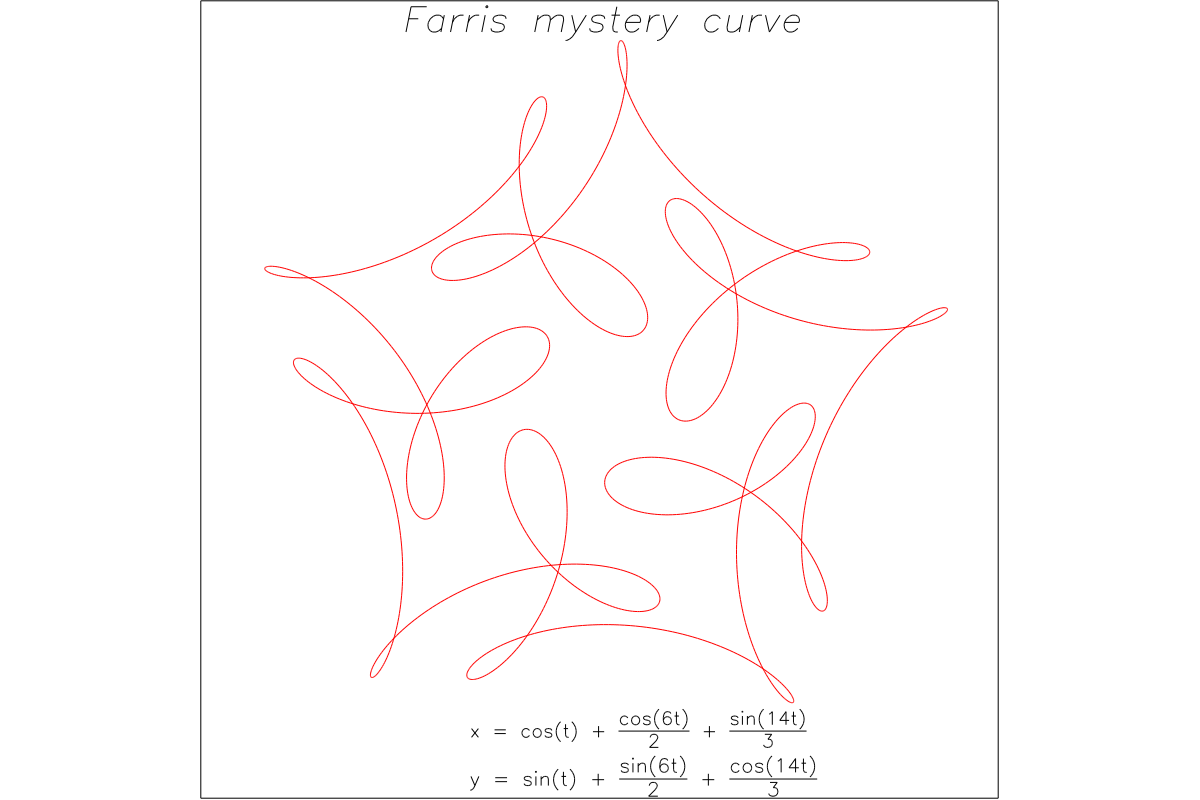
\includegraphics[width=\maxwidth]{../../temp/g1fm001.eps}
  \caption{The Farris Mystery Curve}
  \label{fig:g1fm001}
\end{figure}

\begin{lstlisting}
# FARRIS MYSTERY CURVE
#
RESET
CANVAS -2 2 -2 2
#
MAXPOINTS 3000
#
EVAL 0,TWPI,2001,XLIN
PROC 2 X,SIN,X,6,*,SIN,2,/,+,X,14,*,COS,3,/,+
PROC 1 X,COS,X,6,*,COS,2,/,+,X,14,*,SIN,3,/,+
EVAL @1,@2,PTHO
#
CSG ALL
COL 0 0 0
MOVE 0  -1.66
CTEXT 1.3 "*LX = COS(T) + *,COS(6T)$,2$. + *,SIN(14T)$,3$." 
MOVE 0  -1.9
CTEXT 1.3 "*LY = SIN(T) + *,SIN(6T)$,2$. + *,COS(14T)$,3$." 
MOVE 0, 1.9
CTEXT 2 "*IF*LARRIS MYSTERY CURVE"
#
OUTLINE BOUNDS
\end{lstlisting}

\newpara
The script that generates this is quite short and simple. The first
\texttt{EVAL} fills the X array (stack level 0) with 0 to 2 pi in 2001
linear steps. Two procedures are then defined (stored in procedure
registers 1 and 2). \texttt{PROC\ 1} calculates X values and
\texttt{PROC\ 2} finds Y values. The second \texttt{EVAL} evaluates
these two procedures in the order that leaves the calculated coordinates
on stack for use by the path drawing operator \texttt{PTHO}.

\newpara
It is easy to plot this curve as a graph (i.e.~with value labelled axes,
etc.) simply by replacing \texttt{PTHO} with operators that set the
calculated X and Y values into the X and Y arrays (stack levels 0 and 1)
used by graph plotting commands (here \texttt{XYLINE}). This is
shown in Figure~\ref{fig:g2fm001}.

\begin{figure}
  \centering
  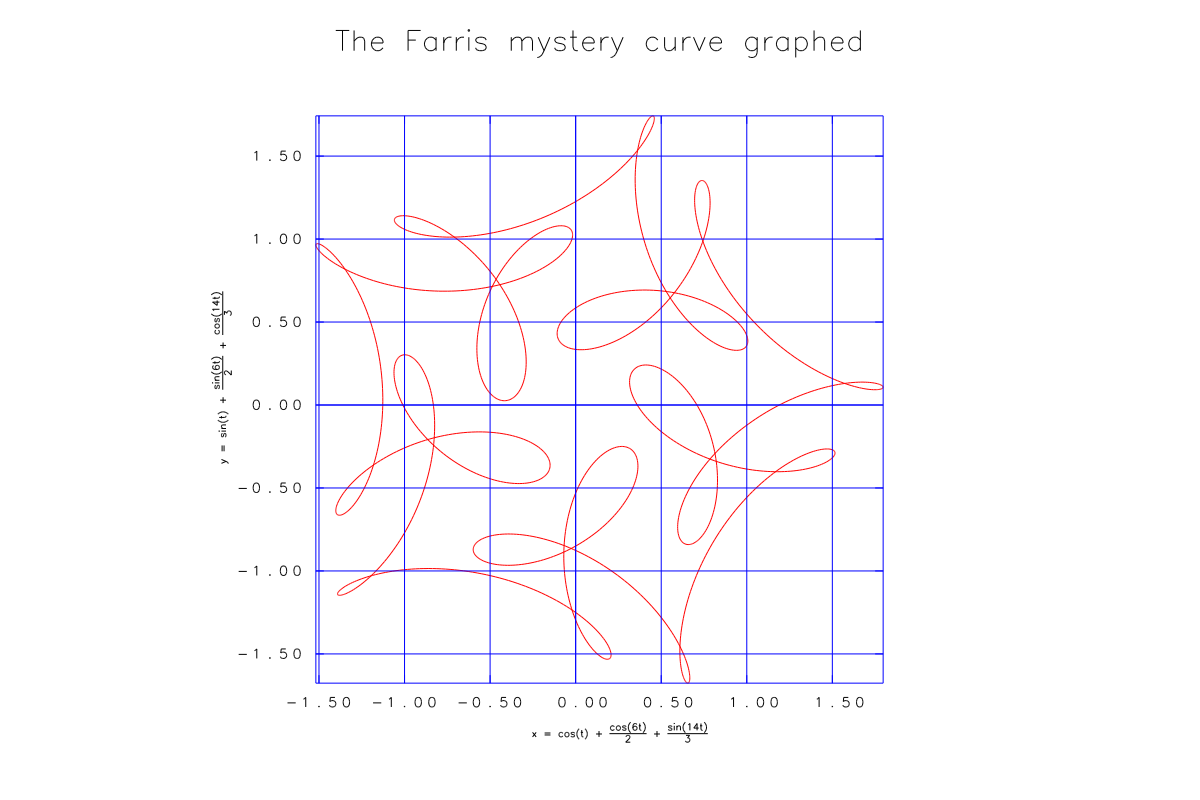
\includegraphics[width=\maxwidth]{../../temp/g2fm001.eps}
  \caption{The Farris Mystery Curve graphed}
  \label{fig:g2fm001}
\end{figure}

\begin{lstlisting}
# FARRIS MYSTERY CURVE PLOTTED AS A GRAPH.
#
CANVAS -2 2 -2 2
#
MAXPOINTS 3000
CSG TEXT
COL 0 0 0
CSG ANNOT
COL 0 0 1
CSG GEN
COL 1 0 0
#
EVAL 0,TWPI,2001,XLIN
PROC 2 X,SIN,X,6,*,SIN,2,/,+,X,14,*,COS,3,/,+
PROC 1 X,COS,X,6,*,COS,2,/,+,X,14,*,SIN,3,/,+
EVAL @1,@2,SETX,POP,SETY
GRAPHMODE OFF
TITLE "T*LHE *UF*LARRIS MYSTERY CURVE GRAPHED"
XLABEL "*LX = COS(T) + *,COS(6T)$,2$. + *,SIN(14T)$,3$."
YLABEL "*LY = SIN(T) + *,SIN(6T)$,2$. + *,COS(14T)$,3$."
GRID BOTH
XYLINE
\end{lstlisting}

\newpara
The Spirograph is a toy invented by Denys Fisher in 1962-64 and fondly
remembered by people of a certain age. It is a simple mechanism which
can trace out hypotrochoid and epitrochoid curves based on two wheels
(with gear teeth, so they can stay in contact without slipping). One
wheel is fixed and the other rotates on the inside or outside of the
fixed wheel. This second wheel has holes in which the tip of a pen can
be placed to draw curves. If the moving wheel rotates inside the fixed
wheel, a hypotrochoid curve is traced out, and if it is outside, an
epitrochoid curve is drawn.

\newpara
Much less accessible mechanisms were developed in the 19th century to
draw such curves for use in banknote engraving as they are visually
attractive and are (or were) difficult to forge without specialised
machinery.

\newpara
Drawing these curves with \textbf{GPLOT} is an interesting exercise. They can be
defined with three integer parameters:

\begin{itemize}
\item
  \texttt{R}, the radius of the fixed wheel.
\item
  \texttt{RL}, the radius of the smaller, moving, wheel.
\item
  \texttt{P}, the distance of the ``pen hole'' from the centre of the
  moving wheel.
\end{itemize}

\newpara
We want to be able to change these easily, so we want to define a script
that we can call like this:

\begin{lstlisting}
OB OBSPIRO "65 25 30"
\end{lstlisting}

\newpara
where we pass the values of \texttt{R}, \texttt{RL} and \texttt{P} to
the script. This is a good opportunity to show how to pass parameters to
scripts and to use ``nested scripts'' to reuse code in the way that
subroutines and functions allow in more sophisticated programming
environments.

\newpara
The script \texttt{OBSPIRO} uses these parameters to calculate how many
times the moving wheel needs to circle the fixed wheel to complete a
closed curve, as well as the degree of symmetry of the curve. Note that
the parameters passed to the script are referred to as \texttt{\$1},
\texttt{\$2}, etc. as they are in Unix scripting languages. Note also
that it is possible to use parameters in the RPN strings used by
\texttt{EVAL}. This can be very useful.

\newpara
One ``problem'' with the parametrised Spirograph simulation is that we
don't know how big the pattern will be -- i.e.~what the range of
coordinates will be -- so we can't easily set the \texttt{BOUNDS} for
the drawing.

\newpara
The \texttt{OBSPIRO} script deals with this using the \texttt{BBSTART},
\texttt{BBEND} and \texttt{BBSET} commands. Between \texttt{BBSTART} and
\texttt{BBEND}, the \texttt{DRAW} command doesn't draw anything (all
drawing ultimately comes down to \texttt{MOVE} and \texttt{DRAW}).
Instead, the range of \texttt{X} and \texttt{Y} coordinates is
accumulated. \texttt{BBSET} can then be used to set these accumulated
ranges as the \texttt{BOUNDS}, optionally scaled about the center by a
scale factor (here, \texttt{1.2}).

\newpara
The tracing out of the Spirograph is done by the script
\texttt{OBSPIRC}, which \texttt{OBSPIRO} ``calls'' twice: once to find
the pattern's bounds and once to draw the pattern.

\newpara
In general, parameters can be passed to obey scripts in two ways:
\begin{itemize}
\item
  Using parameters as described above, where, for example,
  \texttt{OB\ X\ "1\ 2\ 3"} results in \texttt{\$1}, \texttt{\$2} and
  \texttt{\$3} in the script \texttt{X} being read as \texttt{1},
  \texttt{2} and \texttt{3} as a result of \emph{text (string)
  substitution}.
\item
  Numerical values and strings can be passed through registers. This is
  necessary if values are calculated by \texttt{EVAL} to be used in a
  ``nested'' script.
\end{itemize}

\newpara
The \texttt{OBSPIRO} script demonstrates all these features.

\begin{lstlisting}
# SPIROGRAPH PATTERNS - OBSPIRO
#
# FOR MORE INFORMATION, SEE:
#   HTTPS://LINUXGAZETTE.NET/133/LUANA.HTML
#   HTTPS://APERIODICAL.COM/2021/12/THE-MATHEMATICS-OF-SPIROGRAPH/
#
RESET

# THE CONTROL PARAMETERS SHOULD ALL BE INTEGERS.
#
# $1 = R = BIG CIRCLE RADIUS
# $2 = RL = LITTLE CIRCLE RADIUS (MOVES AROUND BIG CIRCLE, IN CONTACT)
# $3 = P = LITTLE CIRCLE PEN RADIUS (FROM CENTRE OF LITTLE CIRCLE)

# THE DEGREE OF SYMMETRY OF THE PATTERN IS MAX(R/GCD(R,RL),RL/GCD(R,RL))

# THE NUMBER OF REVOLUTIONS AROUND THE BIG CIRCLE NEEDED TO JOIN
# UP TO THE START OF THE PATTERN IS:
# NR = RL / GCD(R,RL) (GCD=GREATEST COMMON DIVISOR)

# THE PARAMETER RANGE NEEDED TO DRAW THE THING IS THEN:
# T = [0:2*PI*NR]
#
# AND:
# X(T) = COS(T) * (R - RL) + COS(((R - RL) / RL) * T) * P
# Y(T) = SIN(T) * (R - RL) - SIN(((R - RL) / RL) * T) * P

# CALCULATE NR AND STORE IN REG 9. SAVE GCD(R,RL) IN REG 8.
# NOTE THE DOUBLE QUOTES ARE NEEDED FOR PARAMETER SUBSTITUTION TO WORK
EVAL "$2,$1,$2,GCD,8,=,/,9,="

# FIND THE DEGREE OF SYMMETRY. STORE IN REG 8.
EVAL "$1,8,#,/,$2,8,#,/,MAX,8,="

# FIND THE BOUNDING BOX AND SET BOUNDS.
BBSTART
OB OBSPIRC "$1 $2 $3"
BBEND
BBSET 1.2

# DRAW THE SPIROGRAPH
CSG GENERAL
COL 1 0 0
WIDTH 2
OB OBSPIRC "$1 $2 $3"

# DRAW ANNOTATION (OR NOT)
# CSG GENERAL
# COL 0 0 1
# WIDTH 2
# CIRCLE 0 0 $1
# EVAL "$1,$2,-,0,$2,C"
# EVAL "$1,$2,-,$3,+,0,$3,20,/,C"
# EVAL "$1,0,M,$1,$3,+,$2,-,$3,20,/,-,0,D"

# ADD A PARAMETER DISPLAY
CSG TEXT
COL 0 0 0
BOUNDS 0 1 0 1
MOVE 0.05 0.05
SYMHT 0.02
TEXT "R=$1, *LR=$2, P=$3"
STRING 9 "S*LYMMETRY="
STRING 8 "(I2)"
EVAL "0.05,0.1,M,9,T,TSC,8,#,8,TVI,TEC"
FONT 2 SCRIPT.SIMPLEX
MOVE 0.8 0.95
SYMHT 0.07
CTEXT 0 "*2S*LPIROGRAPH!"
FONT 2 SERIF.COMPLEX

CSG GEN
COL 0 0 0
OUTLINE BOUNDS
\end{lstlisting}

\newpara
The \texttt{OBSPIRC} script does the actual work of calculating pattern
coordinates and drawing the result.

\begin{lstlisting} 
# SPIROGRAPH PATTERN CORE - OBSPIRC

# $1 = R = BIG CIRCLE RADIUS
# $2 = RL = LITTLE CIRCLE RADIUS (MOVES AROUND BIG CIRCLE, IN CONTACT)
# $3 = P = LITTLE CIRCLE PEN RADIUS (FROM CENTRE OF LITTLE CIRCLE)
# REG 9 = NR = NUMBER OF REVOLUTIONS AROUND BIG CIRCLE
#
# T = [0:2*PI*NR]
#
# X(T) = COS(T) * (R - RL) + COS(((R - RL) / RL) * T) * P
# Y(T) = SIN(T) * (R - RL) - SIN(((R - RL) / RL) * T) * P

STO 1 $1
STO 2 $2
STO 3 $3
MAXPOINTS 3000

ERANGE 1 0 6.28 2001
EVAL 0,TWPI,2001,XLIN,X,9,RCL,*,SETX
EVAL 1,RCL,2,RCL,-,5,STO  ; [5] = R - RL
EVAL 5,RCL,2,RCL,/,6,STO  ; [6] = (R - RL)  / RL
PROC 1 X,COS,5,RCL,*,6,RCL,X,*,COS,3,RCL,*,+ ; X
PROC 2 X,SIN,5,RCL,*,6,RCL,X,*,SIN,3,RCL,*,- ; Y
EVAL @1,@2,PTHO
\end{lstlisting}

\newpara
This is quite similar to the ``Farris Mystery Curve'' script in its
approach. Note that it stores the parameters it receives in registers
for use in the RPN, although direct substitution could be used. It first
generates an angle parameter at 2001 points that ``goes around'' the
required number of times to generate a closed pattern, then it finds the
path coordinates based on the angle and draws the result with the open
path operator, \texttt{PTHO}.

\newpara
Figures\ref{fig:g1sp001}, \ref{fig:g2sp001} and \ref{fig:g3sp001} are some examples
of the output of \texttt{OBSPIRO} with different
parameter sets.

\begin{figure}
  \centering
  
\includegraphics[width=\maxwidth]{../../temp/g1sp001.eps}
  \caption{Spirograph Example 1}
  \label{fig:g1sp001}
\end{figure}

\begin{figure}
  \centering
  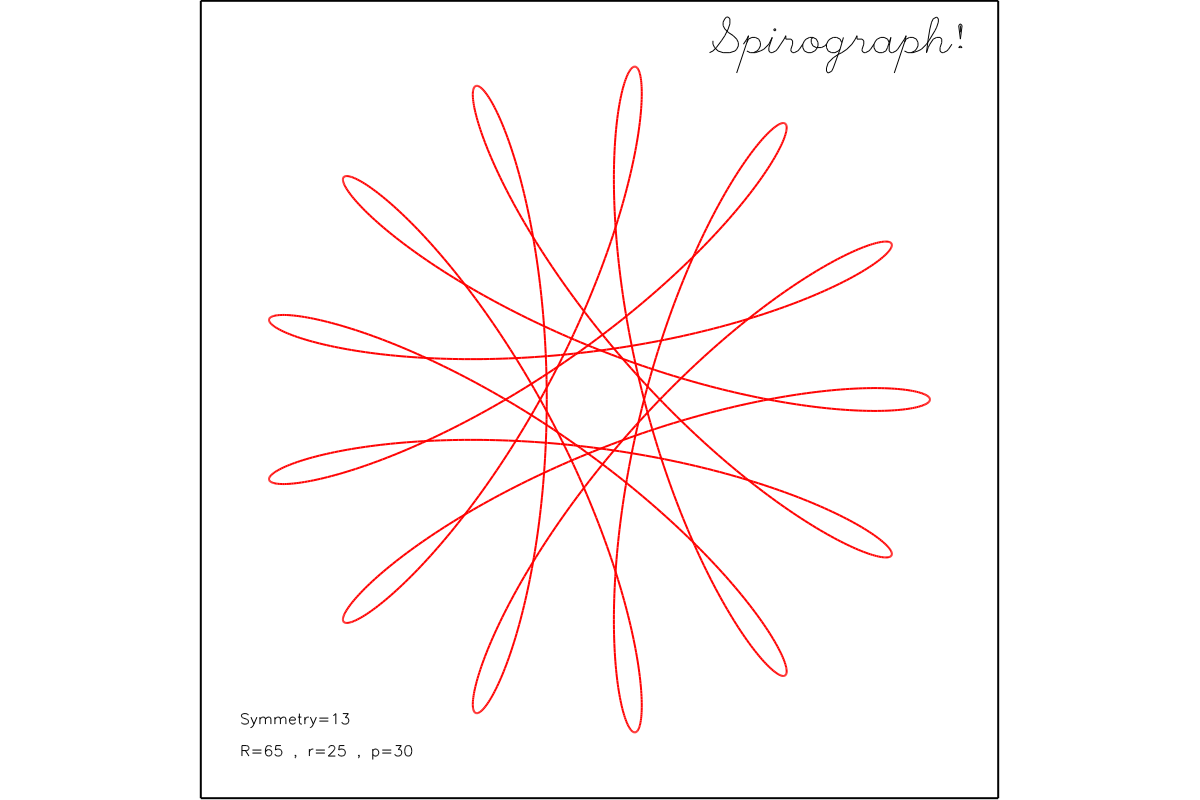
\includegraphics[width=\maxwidth]{../../temp/g2sp001.eps}
  \caption{Spirograph Example 2}
  \label{fig:g2sp001}
\end{figure}

\begin{figure}
  \centering
  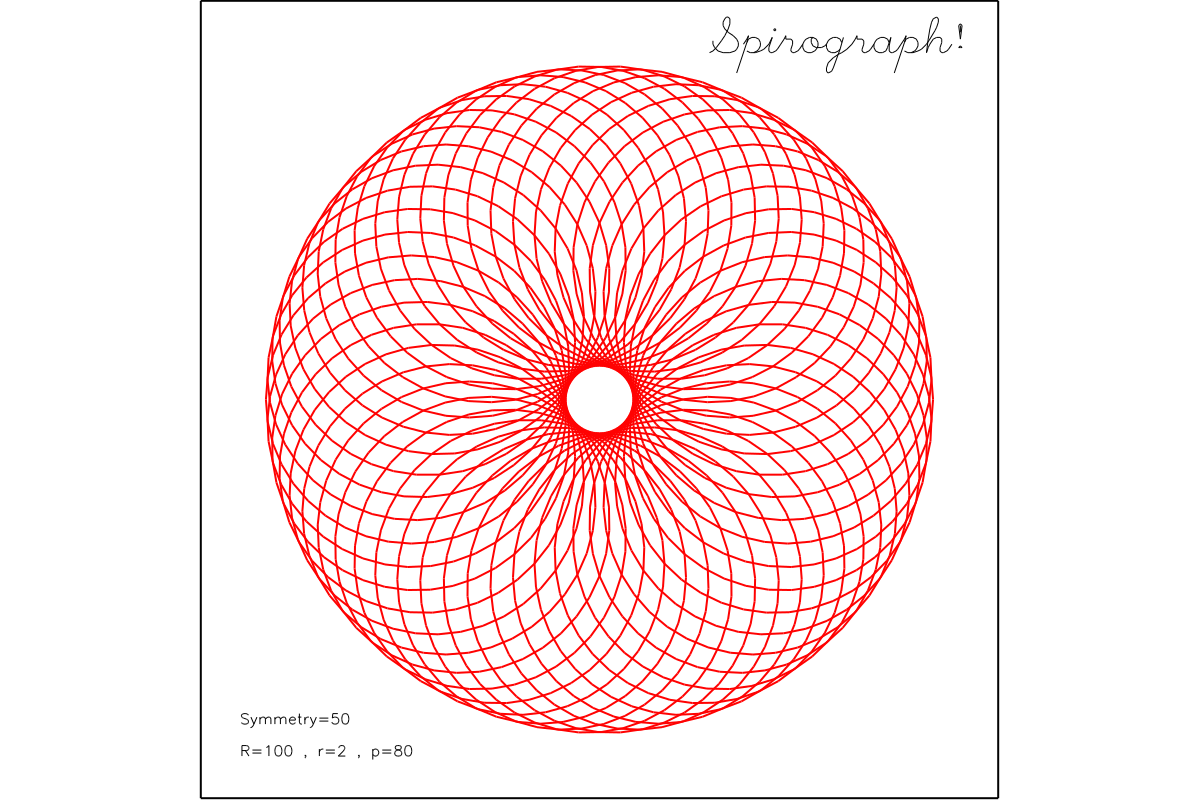
\includegraphics[width=\maxwidth]{../../temp/g3sp001.eps}
  \caption{Spirograph Example 3}
  \label{fig:g3sp001}
\end{figure}

\newpara
Still sticking with procedurally generated patterns, but moving away
from traditional continuous functions of a variable, there is a
traditional form of Japanese Sashiko stitching called Hitomezashi,
developed in the Edo period.

\newpara
These stitch patterns consist of short stitches of a single unit length,
made either horizontally or vertically. If two random sequences of
length \texttt{N} are generated, one for the horizontal direction and
another for the vertical, and a stitch is made if the value of the
sequence is odd (and not made if it is even) then a very attractive
pattern results.

\newpara
I came across this thanks to this
\href{https://www.youtube.com/watch?v=JbfhzlMk2eY}{Numberphile}, video
on YouTube, which gives an excellent explanation of things.

\begin{figure}
  \centering
  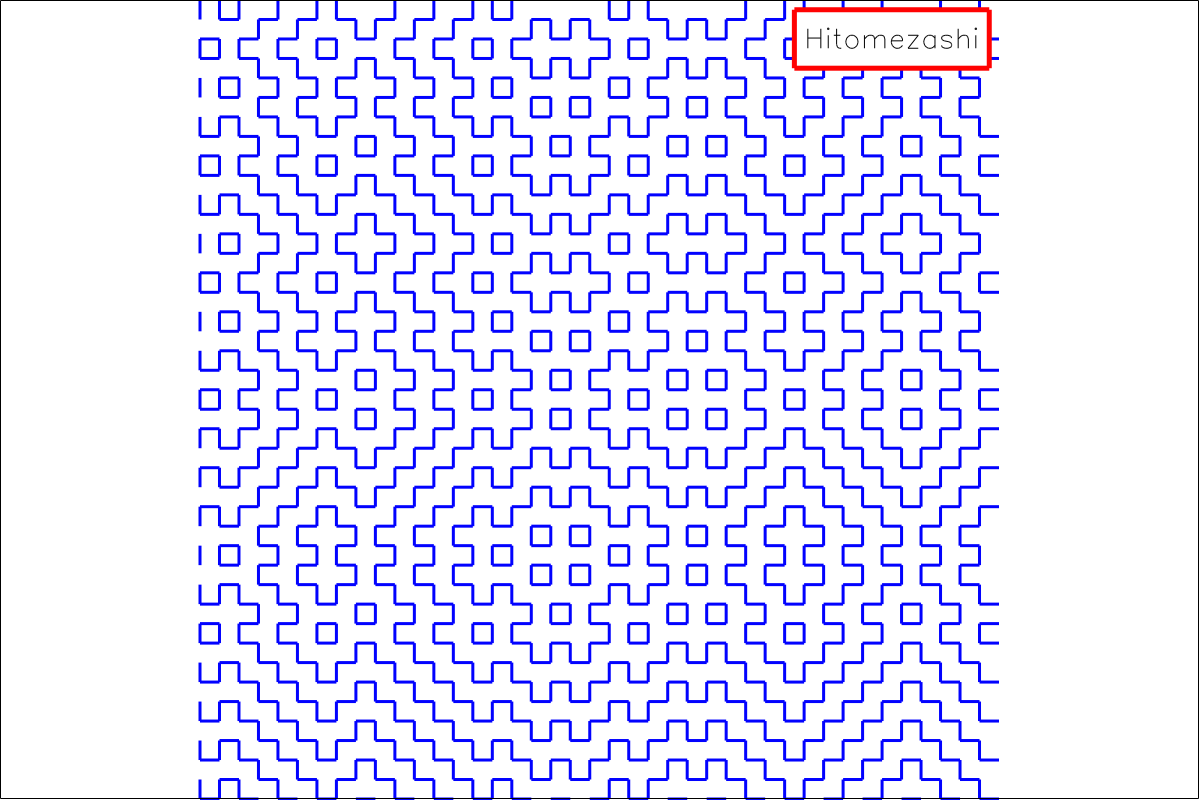
\includegraphics[width=\maxwidth]{../../temp/gemz001.eps}
  \caption{A Hitomezashi stitch pattern}
  \label{fig:gemz001}
\end{figure}

\newpara
The following obey script draws such patterns:

\begin{lstlisting}
# GENERATE HITOMEZASHI STITCH PATTERNS
#
RESET
CANVAS 0 41 0 41
BLANK 30.5 40.5 37.5 40.5

ERANGE 1 0 40 41
PROC 1 1,RAND,0.5,+,FLR,1,EL,X,+,ODD
EVAL 333,SEED

CSG GEN
COL 0 0 1
WIDTH 3
ITEVAL 0 40 1 0,I,M,@1,HDSH
ITEVAL 0 40 1 I,0,M,@1,VDSH

CSG ANNOT
COL 1 0 0
WIDTH 5
OUTLINE BLANK

UNBLANK
MOVE 35.5 39
CSG TEXT
COL 0 0 0
WIDTH 1
CTEXT 9 "H*LITOMEZASHI"

OUTLINE DEV
\end{lstlisting}

\newpara
This introduces a new version of \texttt{EVAL} -- iterated evaluation or
\texttt{ITEVAL}. This repeatedly runs an RPN procedure with a ``loop
variable'' that iterates from a start value to a stop value (inclusive --
Fortran DO-loop rules apply) by a step value. The ``loop variable''
value can be accessed inside the RPN using the \texttt{I} operator.

\newpara
This example also shows how to use \texttt{BLANK} and \texttt{UNBLANK}
to temporarily protect a rectangular region so that it cannot be drawn
in.


\subsection{General drawing - Part 2: Evaluator assisted}\label{general-drawing---part-2-evaluator-assisted}

\newpara
It is possible to use the evaluator to assist with general drawing
tasks. In many cases, it is necessary to calculate coordinates from a
small set of supplied parameters in order to complete the drawing task.
A good example of this was the ``labelled angle line pair'' shown in the
manual general drawing section, where we used a calculator to find the
coordinates of the label text literally by hand.

\newpara
Probably the most convenient way of using the evaluator for such tasks
is to add procedures to the \emph{evaluator procedure library} which
consists of the file \texttt{GPLPROC} (\texttt{gplproc} on Unix-like
systems).

\newpara
The procedures in this library are, to some extent, a way to extend
\textbf{GPLOT's} capabilities, or, at least, make some things much more
convenient than they otherwise would be.

\newpara
The contents of \texttt{GPLPROC} include comments that document its
procedures. Please read it for full information. To understand its
features, here are a couple of examples.

\newpara
This \texttt{RELLIPSE} procedure draws an ellipse (which \textbf{GPLOT/DIMFILM}
cannot do directly). It has five parameters, the center position
\texttt{(XC,YC)}, the semi-major and semi-minor axis lengths and a
rotation angle (a rotation of the ellipse axes).

\begin{lstlisting}
C A ROTATED ELLIPSE "XC YC A B ANGLE-DEGREES"
RELLIPSE
CL,0,TWPI,360,XLIN,X,&,COS,S,SIN,3,#,4,#,SCL,5,#,D2R,ROT,1,#,2,#,TRN,PTHC
\end{lstlisting}

\newpara
To use this procedure to draw a rotated ellipse, two \textbf{GPLOT} commands are
needed:

\begin{lstlisting}
LOAD 1 RELLIPSE
EVAL @1 "5,1,0.5,0.9,33"
\end{lstlisting}

\newpara
The first line loads the required procedure into a procedure register (1
here), then the second executes it, passing it the required arguments.
If a given procedure is to be ``called'' multiple times, it need only be
loaded once, of course.

\newpara
The second example shows a useful feature unique to \texttt{GPLPROC}. A
major limitation of the evaluator is that RPN strings are limited to 80
characters. This is not enough for many ``real world'' applications.
When a procedure is loaded from \texttt{GPLPROC}, it can span multiple
lines. In such a case, the procedure is loaded into multiple successive
procedure registers and \texttt{,@n} sequences are automatically added
to line ends so that the when the procedure is called from an
\texttt{EVAL} command, a single long procedure is assembled and
executed. A side effect of this scheme is that lines can be no more than
77 characters long if another line follows in the procedure definition.

\begin{lstlisting}
C GEAR "X Y R1 R2 N-TEETH ROT-DEGREES"
GEAR 2
CL,0,5,#,&,1,+,XLIN,3,#,4,#,X,2,/,ODD,SEL,X,TWPI,*,5,#,/,6,#,D2R,+,&
COS,S,SIN,3,G,*,S,3,G,*,1,#,2,#,TRN,PTHO
\end{lstlisting}

\newpara
Note that the number of lines in the full procedure (2 here) must be
given after the procedure name. These procedures must be loaded into a
procedure register number that leaves enough successive registers to
hold the full thing. Here, for example, \texttt{LOAD\ 8\ GEAR} would
work, but \texttt{LOAD\ 9\ GEAR} would not.

\newpara
The script \texttt{OBPRTST} calls every procedure currently defined in
\texttt{GPLPROC} as shipped. The output of that is shown in
Figure~\ref{fig:gdea001}.

\begin{figure}
  \centering
  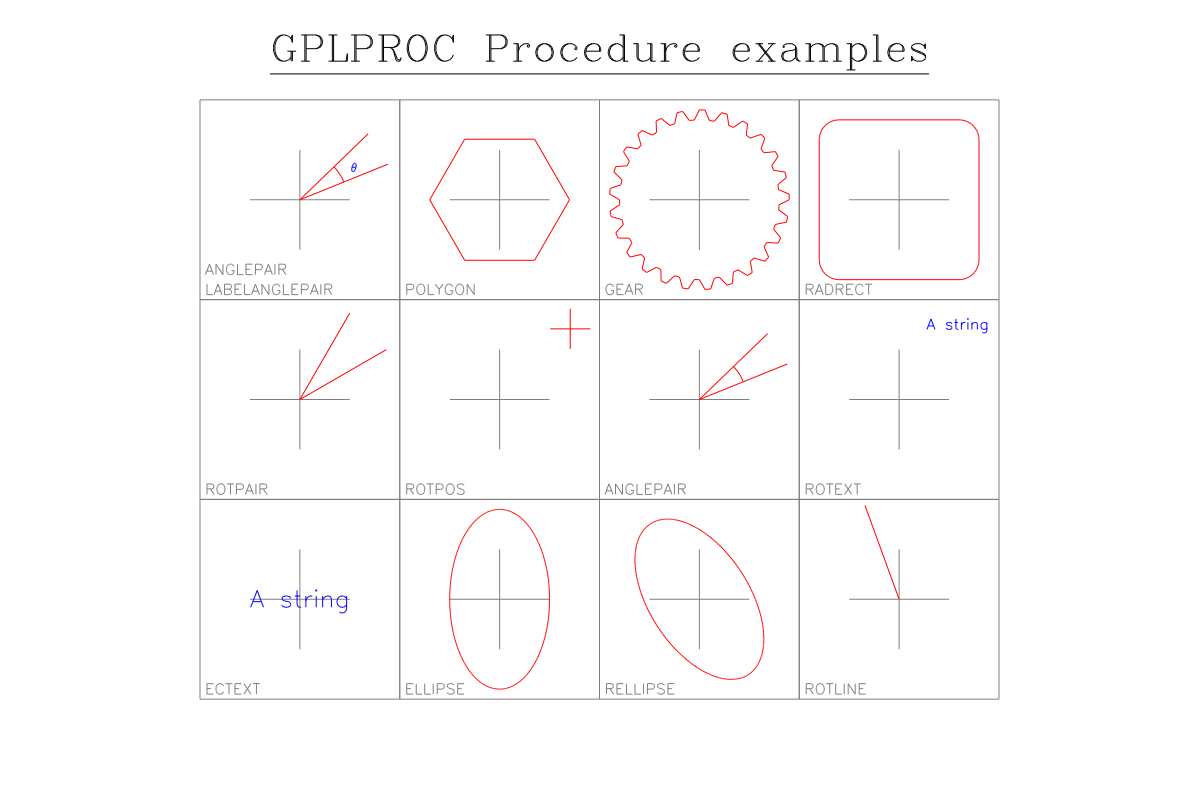
\includegraphics[width=\maxwidth]{../../temp/gdea001.eps}
  \caption{Examples of each procedure in \texttt{GPLPROC}}
  \label{fig:gdea001}
\end{figure}

\newpara
It is intended that \textbf{GPLOT} users add their own procedures to
\texttt{GPLPROC} to ``extend'' \textbf{GPLOT} to do things they want to do.

\subsection{General drawing - Part 3: Higher level drawing}\label{general-drawing---part-3-higher-level-drawing}

\newpara
Although the evaluator can ``extend'' the capabilities of \textbf{GPLOT} to some
extent, it has some pretty severe limitations and inconveniences. The
main limitations are the maximum size of procedures and the complete
lack of branching and looping features. In practice, you cannot ``draw
anything'' with \textbf{GPLOT/DIMFILM} in the way that you can with PostScript,
for example.

\newpara
There are some drawing operations beyond the (very) basic facilities
described above which are sufficiently generally useful to ``build in''
to \textbf{GPLOT}. This hopefully makes it relatively easy to draw things that
are commonly useful (easier than using PostScript, for example), while
acknowledging that there are still fundamental limitations to what can
be drawn.

\newpara
To this end, \textbf{GPLOT} has three ``higher level'' drawing ``primitives'':

\begin{itemize}
\item
  Decorated lines
\item
  Boxed text
\item
  Labels with pointing arrows.
\end{itemize}

\newpara
These can be used for a broad range of diagrams, but especially block
diagrams.

\newpara
A \textbf{decorated line} is a series of connected and directed line
segments, the ends of which may have:

\begin{itemize}
\item
  Arrow heads. These will automatically point in the correct direction
  (hopefully).
\item
  ``Half skips''. These are (close to) quarter circles, and if a line
  ends and begins with one of these, it can give the appearence of
  skipping over another line, as was commonly seen in older circuit
  diagrams.
\item
  No decorations or ``plain''.
\end{itemize}

\newpara
Such a line is drawn by the \texttt{LINE} command which takes a string
that defines the line segments and their decorations. Each coordinate or
\emph{point description} defining a ``vertex'' in the ``polyline'' has
the following components:

\begin{lstlisting}
<decoration>x,y[,<annotation_string>]

<decoration> = P (plain) or A (arrow) or S (half skip)

<annotation_string> is a short string (currently limited to 5 characters).
It may contain \textbf{DIMFILM} string markup. It cannot contain spaces.
\end{lstlisting}

\newpara
The annotation string, if supplied, will be drawn in a circle at the
mid-point of the line segment ended by the point description that
specifies it. This is intended to be a \emph{very short} label.

\newpara
The point descriptions are separated by \texttt{"\textgreater{}"}
characters, which can be read in this context as ``to''.

\newpara
Here is an example that defines a two segment decorated line, starting
with no decoration and ending in an arrow head with a label,
\texttt{"Le"}, in the middle of the first of the two line segments:

\begin{lstlisting}
LINE P7,6>P7,21,L*LE>A16,21
\end{lstlisting}

\newpara
Additional characteristics of decorated lines are specified by the
\texttt{ARROWPARM} and \texttt{LINEPARM} commands. The latter sets scale
factors for drawing skips and annotations, while the former sets the
type, size and appearance of arrow heads. Note that the width and colour
of decorated lines are set in the usual way (lines, arrows and skips are
in \texttt{CSG\ GENERAL}, annotation text in \texttt{CSG\ TEXT}).

\newpara
\textbf{Boxed text} is intended to be a fairly flexible component for
constructing block diagrams, tables and many other drawings. The element
is basically text centered in a box of a specified size at a specified
position (given either by centre or bottom left).

\newpara
A number of other features can be added, though.

\begin{itemize}
\item
  The inside of the box can be ``filled'' with hatched lines.
\item
  A second box, inside the first and surrounding the text, can be drawn.
  It is a \texttt{BLANK} region, and it can be outlined.
\item
  The text may have multiple lines (up to 5), separated by backslashes.
\item
  The text may be centered or left justified.
\item
  The text can contain \textbf{DIMFILM} string markup.
\item
  The position of the boxed text can be automatically ``stepped'' by
  specified X and Y ``deltas'' after eah one is drawn. This makes it
  much easier to use this for constructing tables and other things.
\end{itemize}

\newpara
The main command for this element is \texttt{BOXTEXT}, which draws a
given text string at a position given by either a supplied coordinate,
or, if the coordinate is omitted, at the position of the last
\texttt{BOXTEXT} incremented by previously specified deltas.

\newpara
A number of secondary commands set current characteristics of
\texttt{BOXTEXT}. These are:

\begin{itemize}
\item
  \texttt{BOXPSIZE} which sets the box size and how the position
  coordinate is to be interpreted.
\item
  \texttt{BOXPHATCH} which sets the hatching parameters (or turns it
  off).
\item
  \texttt{BOXPTEXT} which sets how text is drawn inside the box. There
  are two distinct modes: \texttt{FIX} and \texttt{SCALE}. In
  \texttt{FIX} mode, the \texttt{WIDTHSCALE} parameter sets how many
  lines will fit in the box height, while in \texttt{SCALE} mode, it
  sets the fraction of the box width the text should be scaled to fill.
\item
  \texttt{BOXPBOX} which controls whether the outer and inner boxes are
  outlined.
\item
  \texttt{BOXPDELTAS} which sets the automatic position step after ecah
  \texttt{BOXTEXT} is drawn.
\end{itemize}

\newpara
\textbf{Labels} are the same graphical entities used to label points on
a graph, but the coordinates of the thing they point at is in bounds
rather than graph coordinates.

\newpara
Figure~\ref{fig:gh1b001} is a simple example of how
these facilities can be used to draw a
small block diagram.

\begin{figure}
  \centering
  
\includegraphics[width=\maxwidth]{../../temp/gh1b001.eps}
  \caption{A simple block diagram}
  \label{fig:gh1b001}
\end{figure}

\begin{lstlisting}
RESET
BOUNDS 0 42 0 26

CSG TEXT
COL 0 0 0
CSG ANNOT
COL 0 0 0
WID 2

BOXPSIZE 10 6 NO

BOXT "B*LOX 1" 7 3
BOXT "B*LOX 2" 21 3
BOXT "C*LURIOUS\*UB*LOX 3" 35 3

BOXT "B*LOX 4" 35 13

BOXPHATCH 0.05 8 HORIZ
BOXPBOX BOTH
BOXT "B*LOX 5\*UA*LN ODDITY" 21 21

CSG GEN
COL 0 0 0
ARROWPARM BARBED 0.8 2 0.3
LINEPARM 0.5 1.5
LINE P12,3>A16,3
LINE P26,3>A30,3
LINE P35,6>A35,10
LINE A35,16>P35,21,R*LT>A26,21
LINE P7,6>P7,21,L*LE>A16,21

LINE P12.5,12.5>P13.2,12.5>A14.1,14.1
ALABEL 13.2 12.5 2 300 "What is this thing?"

OUTLINE DEVICE
\end{lstlisting}

\newpara
It may look painful to create a diagram such as this by entering
coordinates, and perhaps it is. However, it may be less painful than it
seems at first. A key simplification is to use an integer coordinate
system with the box size a useful multiple of the unit size (e.g.~so
that middle of the box edges is easy to find). It is also helpful to
have a grid printed out (!) with the coordinate system shown over a
specified range (\texttt{BOUNDS}). As an aid to this, the script
\texttt{OBGRID} can draw such a grid which can be used as the background
of the diagram as it is developed (e.g.~using the \textbf{GTerm} device)
or printed to help sketch out the diagram.
An example of the use of a grid is shown in Figure~\ref{fig:ghbb001}.

\newpara
Surely it would be easier to just use, say, Inkscape? Perhaps. I have
drawn many block diagrams with Inkscape and in some ways it is obviously
easier. But it still takes longer than might be expected to get to a
``final'' result. It is also very difficult (at least for me) to get
lines and boxes to ``snap'' together precisely (I usually give up on
perfecting this, to be honest). The \textbf{GPLOT} approach at least results in
exact alignment of all elements! In summary, I'm not sure it is all that
more time consuming to get to an acceptable result. Which approach you
prefer (using a mouse and relying on hand/eye coordination or working
out and typing in coordinates) is a matter of personal taste. Obviously,
if you want to draw a portrait of your dog, Inkscape (or a similar
program) is the only sane choice! For more exactly defined tasks, a
``language based'' approach can make sense, as proved by the success of
vector graphics description languages such as PGF/Tikz.

\begin{figure}
  \centering
  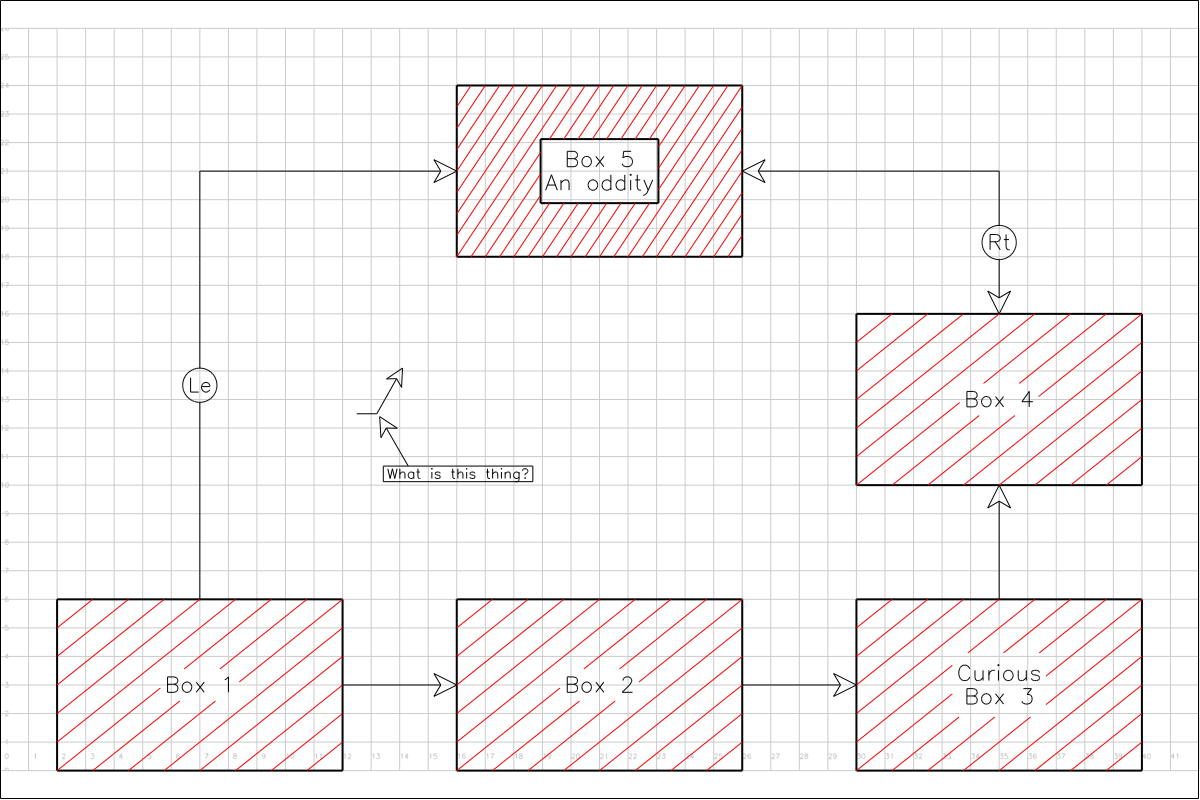
\includegraphics[width=\maxwidth]{../../temp/ghbb001.eps}
  \caption{Using a grid to assist with planning a block diagram}
  \label{fig:ghbb001}
\end{figure}

\begin{lstlisting}
#
# DRAW A GRID WITH NUMBERED AXES. USEFUL FOR BLOCK DIAGRAMS.
# CALL WITH BOUNDS AS PARAMETERS.
#
BOUNDS $1 $2 $3 $4
CSG ALL
COL 0.8 0.8 0.8
STRING 9 "(I2)"
ITEVAL $3 $4 1 "$1,I,M,$2,I,D"
ITEVAL $1 $2 1 "I,$3,M,I,$4,D"
ITEVAL $3 $4 1 "$4,$3,-,100,/,TH,$1,I,M,I,9,TVI"
ITEVAL $1 $2 1 "$4,$3,-,100,/,TH,I,$3,0.5,+,M,I,9,TVI"
\end{lstlisting}

\newpara
For a more sophisticated example of a block diagram drawn with \textbf{GPLOT},
look at the script \texttt{OBMODIO} which draws the block diagram at the
top of the Github \texttt{README.md} document showing
the component parts of the Git-MODIFY
inter-operability scheme. This is shown in Figure~\ref{fig:iocd001}.

\begin{figure}
  \centering
  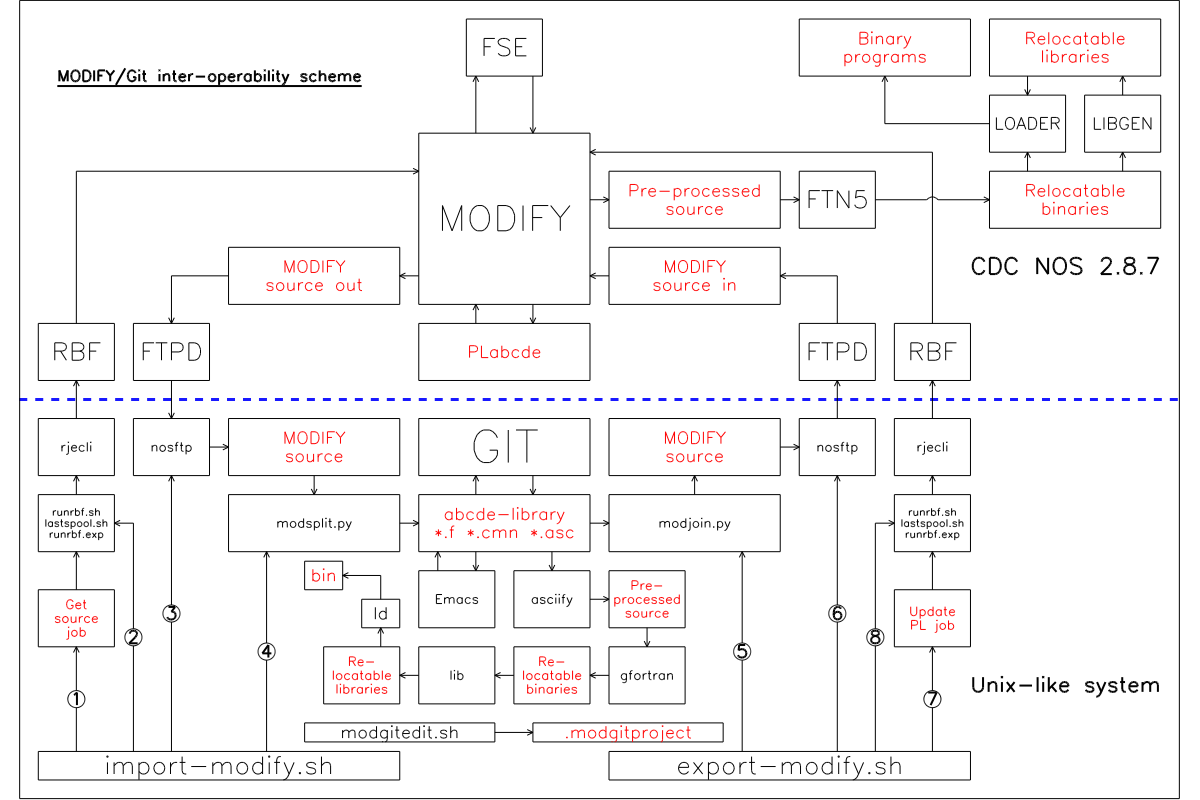
\includegraphics[width=\maxwidth]{../../temp/iocd001.eps}
  \caption{Git-MODIFY Inter-operability scheme components diagram}
  \label{fig:iocd001}
\end{figure}

\newpara
An example of using \textbf{GPLOT} (primarily \texttt{BOXTEXT}) to produce a
drawing other than a block diagram is shown below. This documents the
key bindings for the NOS 2 Full Screen Editor with a Macbook laptop
keyboard.

\begin{figure}
  \centering
  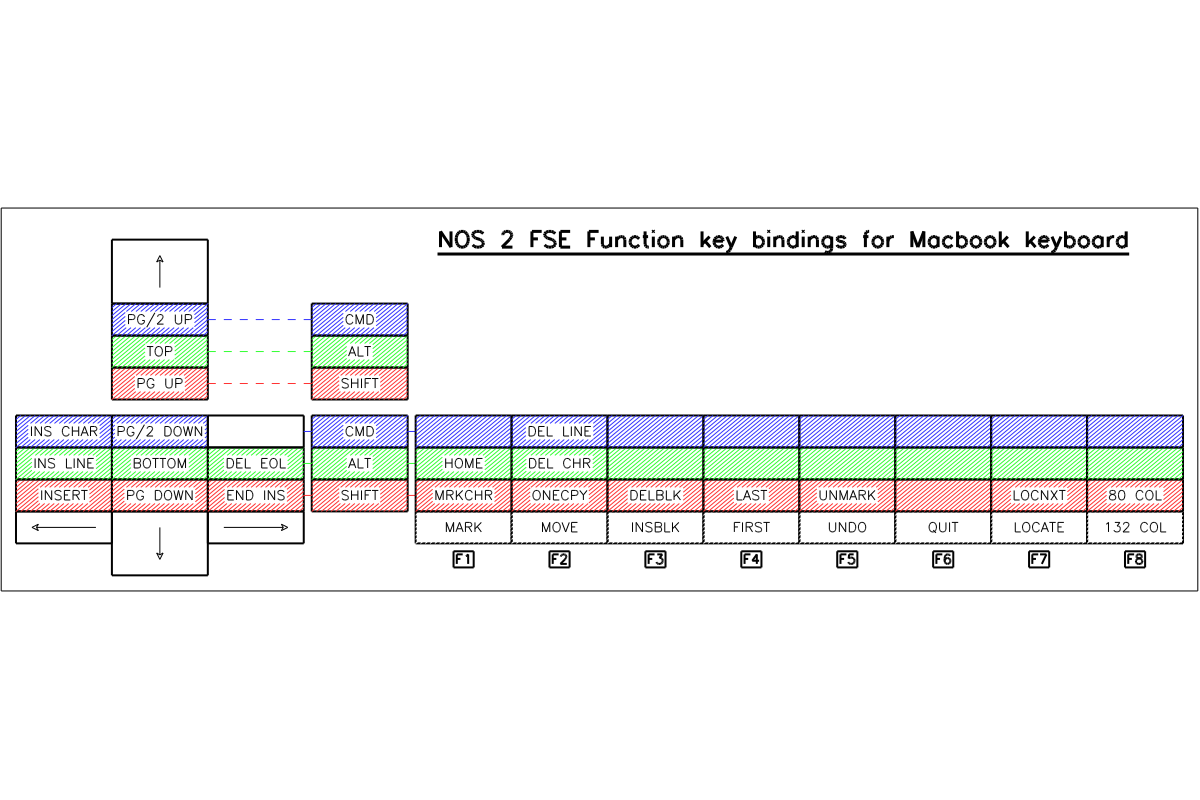
\includegraphics[width=\maxwidth]{../../temp/gh2b001.eps}
  \caption{A diagram showing the key layout for FSE on a MacBook}
  \label{fig:gh2b001}
\end{figure}

\newpara
Further examples of how the ``higher level drawing'' features can be
used can be seen in the \texttt{OBCHT1} and \texttt{OBCHT2} scripts
which generate the \textbf{GPLOT} ``cheat sheet'' which can be found at the end
of this document.

\subsubsection{L-Systems}\label{l-systems}
\newpara
L-systems or Lindenmeyer systems are a type of formal grammar (as in
mathematical logic) developed by Aristid Lindenmeyer, a theoretical
biologist, in 1968 to model the processes of plant development. They can
be used to generate a variety of attractive images, beyond plants and
trees, including self-similar fractals. See this
\href{https://en.wikipedia.org/wiki/L-system}{Wikipedia} article for
more background information.

\newpara
Lindenmeyer systems generating 2D vector graphics are included in \textbf{GPLOT}.
The implementation is based on Paul Bourke's description of a 1991
commercial product (probably now long dead) which can be found
\href{https://paulbourke.net/fractals/lsys/}{here}. As with many of Paul
Bourke's web pages, this is very informative and inspirational.

\newpara
L-systems work by manipulating strings, the characters of which either
represent graphical actions (such as moving forward, drawing a line, or
turning through an angle) or are ``variables'' with no associated
graphical meaning.

\newpara
An L-system is defined by an ``axiom string'' and a set of ``re-writing
rules'', and, in our case, also a fixed ``turning angle''. The ``axiom
string'' must be set in string register 1 and up to 8 ``re-writing
rules'' can then appear in string registers 2 to 9 (used consecutively).
The initial line angle is set by storing the angle (in degrees) in
numeric register 3.

\newpara
The characters allowed (``vocabulary'') are:
\texttt{F\ A\ B\ C\ D\ E\ M\ X\ Y\ +\ -\ {[}\ {]}} Seven of these are
associated with specific actions. Any alphabetic character can be
substituted with a string by a re-writing rule. The seven ``action
characters'' are:

\begin{itemize}
\item
  \texttt{F} - draw a unit length line segment at the current drawing
  angle.
\item
  \texttt{D} - as \texttt{F}, but some systems need two substitutable
  drawing characters.
\item
  \texttt{M} - move by a unit length at the cureent drawing angle.
\item
  \texttt{+} - turn counter-clockwise by the turning angle.
\item
  \texttt{-} - turn clockwise by the turning angle.
\item
  \texttt{{[}} - push the current position and drawing angle on a stack.
\item
  \texttt{{]}} - pop the current position and drawing angle off a stack.
\end{itemize}

\newpara
This is all very abstract, of course! Paul Bourke's web page gives a
simple example which is quite easy to follow, but more complex systems
are not obvious (to me, anyway).

\newpara
Figure~\ref{fig:lsys001} is a classic example of a plant drawn with an L-system,
drawn by the following script.

\begin{figure}
  \centering
  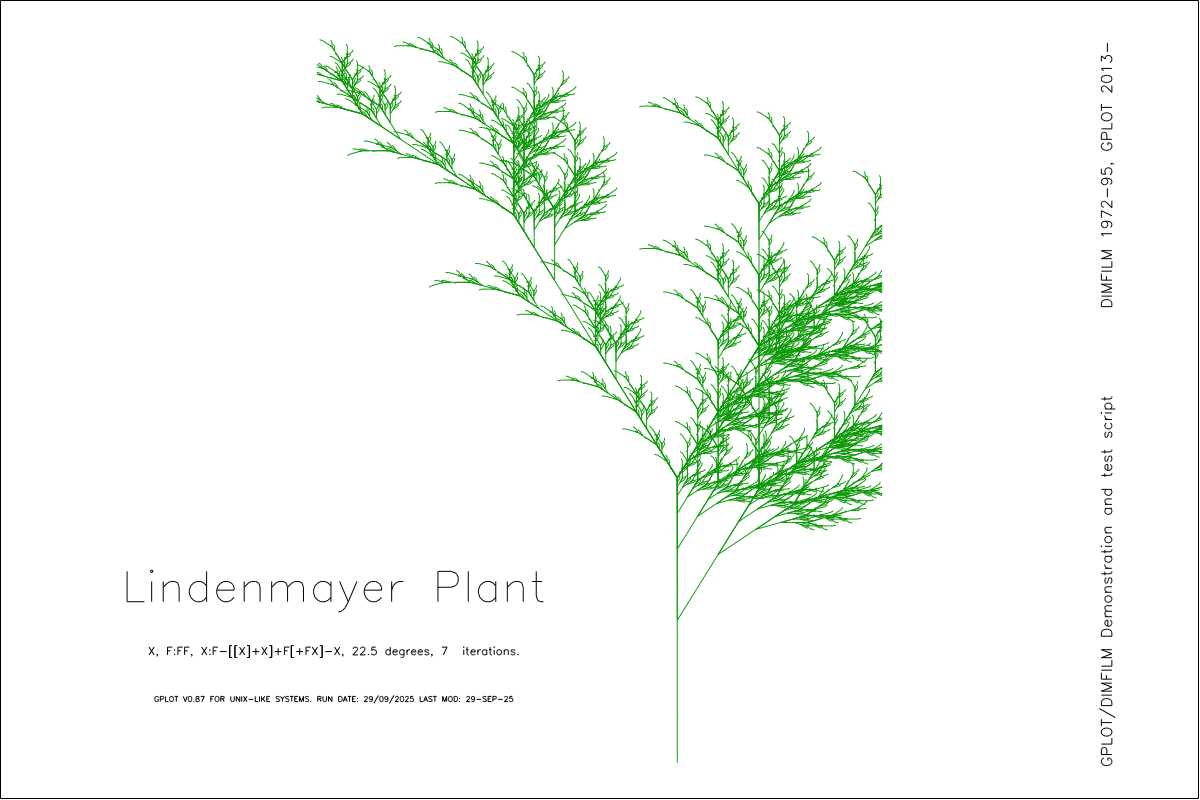
\includegraphics[width=\maxwidth]{../../temp/lsys001.eps}
  \caption{A Lindenmeyer plant also demonstrating other facilities}
  \label{fig:lsys001}
\end{figure}

\begin{lstlisting}
# PROCEDURE TO DRAW AN ALGORITHMICALLY DEFINED
# PLANT USING A LINDENMAYER SYSTEM.
# USAGE:
#  OBEY OBPLANT <ITERATIONS>
#   ITERATIONS BETWEEN 5 AND 8 SEEMS REASONABLE.

# INITIALISE GPLOT STATE.
RESET
GRAPHMODE ON

# SET THE COLOUR OF THE PLANT.
CSG GENERAL
COL 0.05 0.6 0.03

# DEFINE THE LINDENMAYER SYSTEM FOR THE PLANT.
STRING 1 X
STRING 2 F:FF
STRING 3 X:F-[[X]+X]+F[+FX]-X 
STO 3 90

# DRAW THE PLANT
LSYSTEM 2 $1 22.5

# SETUP TO ADD ANNOTATION
GRAPHMODE OFF
BOUNDS 0 1.33 0 1
CSG TEXT
COL 0 0 0

# DEMONSTRATE CTEXT CENTRED TEXT.
MOVE 0.3325 0.265
CTEXT 0.532 "L*LINDENMAYER *UP*LLANT"
MOVE 0.3325 0.185
CTEXT 0.4655 "X, F:FF, X:F-[[X]+X]+F[+FX]-X, 22.5*L DEGREES, $1 ITERATIONS."

# DEMONSTRATE ROTATED TEXT VIA THE RPN EVALUATOR.
STRING 5 "GPLOT/DIMFILM D*LEMONSTRATION AND TEST SCRIPT"
STRING 6 "  DIMFILM 1972-95, GPLOT 2013-"
EVAL "1.31,0.05,M,90,TA,5,T,1.31,0.6,M,6,T"

# ADD THE GPLOT VERSION INFO, DRAWING CENTRED TEXT
# VIA A STORED PROCEDURE.
VERSION 9
LOADP 1 ECTEXT
EVAL @1 "0.3325,0.125,0.45,9"

OUTLINE DEV
\end{lstlisting}

\newpara
Note that, in general, the complexity of the drawing explodes as the
number of iterations increases. The \textbf{GPLOT} L-system implementation uses
scratch files to avoid memory limitations on NOS, so large outputs are
possible, but the compute times also explode! The maximum stack depth is
set to 20, although this doesn't seem to be much of a limitation in
practice.

\newpara
Here are some other examples.

\newpara
A complicated, bristly plant (Figure~\ref{fig:lsbr001}) is
drawn by the following script.

\begin{figure}
  \centering
  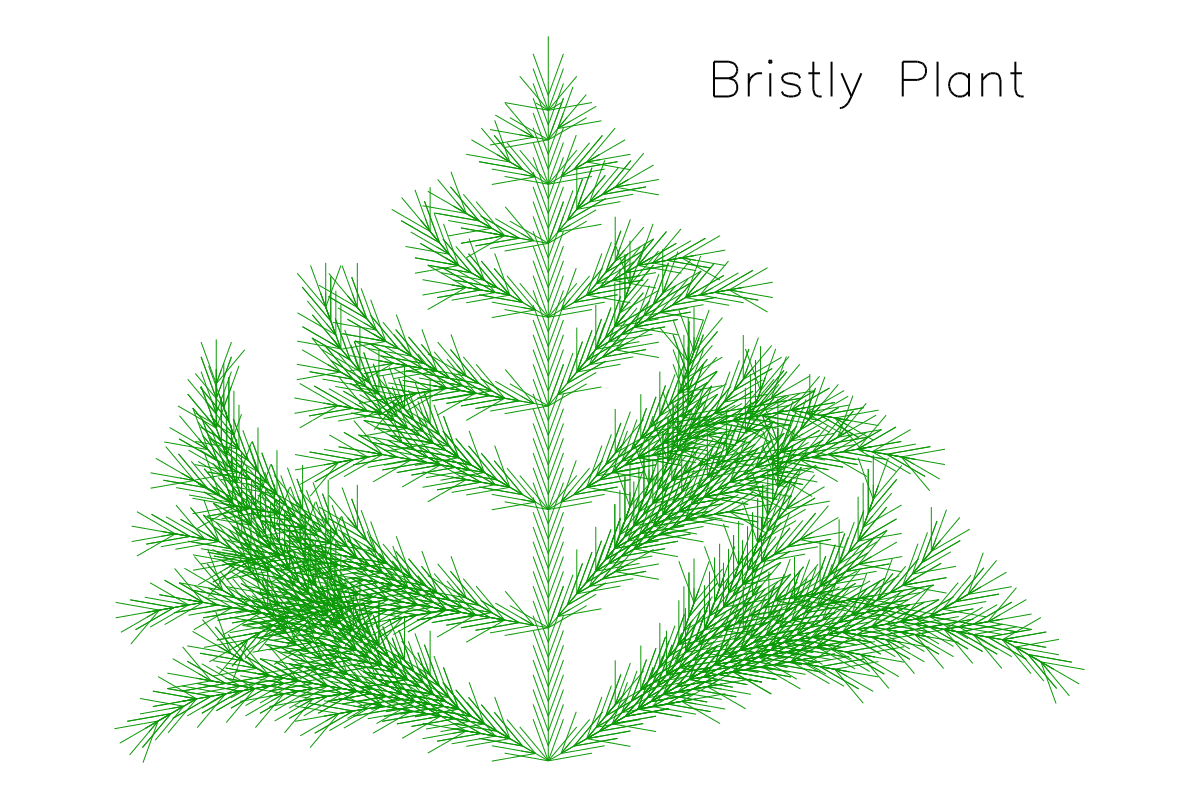
\includegraphics[width=\maxwidth]{../../temp/lsbr001.eps}
  \caption{A bristly looking plant}
  \label{fig:lsbr001}
\end{figure}

\begin{lstlisting}
RESET

# SET THE COLOUR OF THE PLANT.
CSG GENERAL
COL 0.05 0.6 0.03

# DEFINE THE LINDENMAYER SYSTEM FOR THE PLANT.
STRING 1 ABFFF
STRING 2 A:[+++C][---C]YA
STRING 3 C:+X[-C]B
STRING 4 X:-C[+X]B
STRING 5 Y:YB
STRING 6 B:[-FFF][+FFF]F

# INITIAL DRAWING ANGLE.
STO 3 90

# DRAW.
LSYSTEM 5 $1 20
\end{lstlisting}

\newpara
Figure~\ref{fig:lssm001} shows a Minkowski island, after 4 iterations.
L-systems can generate most
(all?) 2D fractal curves. Several such curves follow.

\begin{figure}
  \centering
  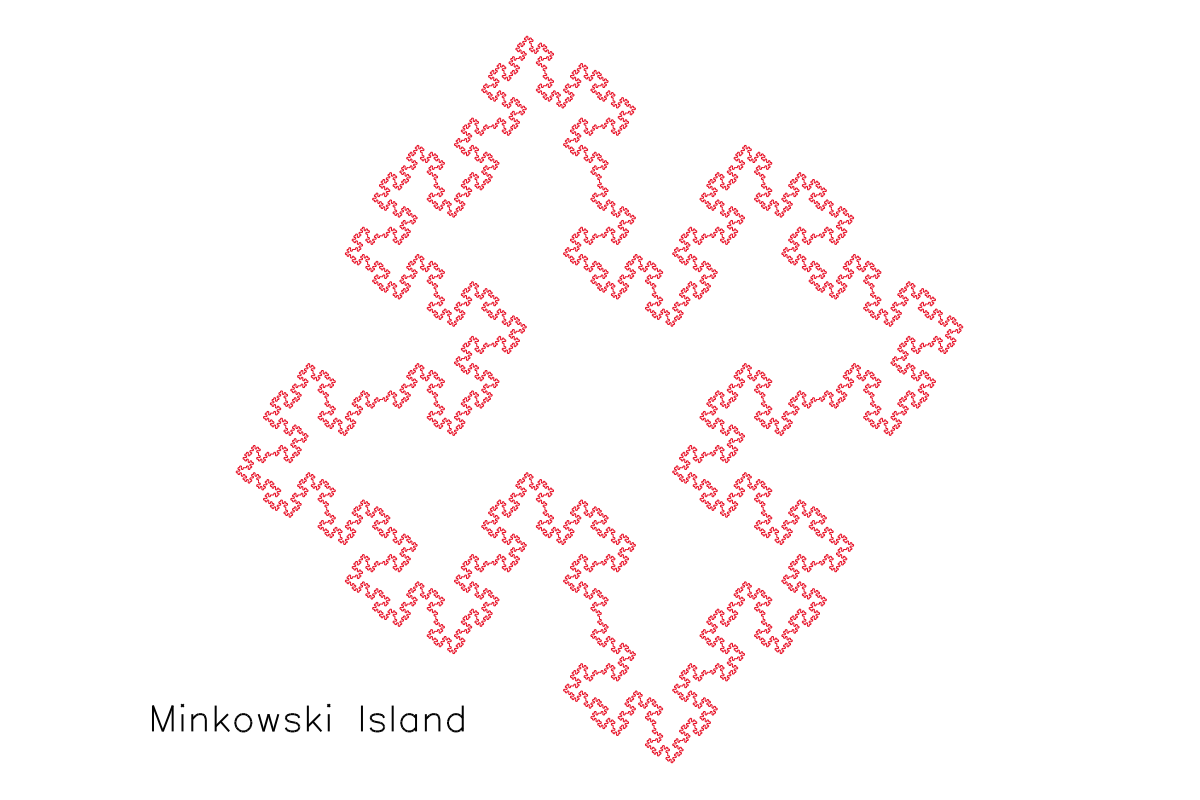
\includegraphics[width=\maxwidth]{../../temp/lssm001.eps}
  \caption{A Minkowski Island (4 iterations)}
  \label{fig:lssm001}
\end{figure}

\begin{lstlisting}
RESET

STRING 1 F+F+F+F
STRING 2 F:F+F-F-FF+F+F-F

STO 3 0

CSG GENERAL
COL 0.9 0 0.1

LSYSTEM 1 $1 90
\end{lstlisting}

\newpara
Figure ~\ref{fig:lssp001} shows a 
Sierpinski gasket after 6 iterations, drawn by this script.

\begin{figure}
  \centering
  \includegraphics[width=\maxwidth]{../../temp/lssp001.eps}
  \caption{A Sierpinski Gasket (6 iterations)}
  \label{fig:lssp001}
\end{figure}

\begin{lstlisting}
RESET

STRING 1 F+F+F        ; AXIOM
STRING 2 F:F-F+F+F-F  ; GENERATOR

STO 3 0               ; INITIAL ANGLE

CSG GENERAL
COL 0.9 0 0.1

# DRAW THE GASKET
LSYSTEM 1 $1 120
\end{lstlisting}

\newpara
Figure~\ref{fig:lsks001} shows a Koch ``snowflake'' drawn with rectangular elements
is drawn by this script.

\begin{figure}
  \centering
  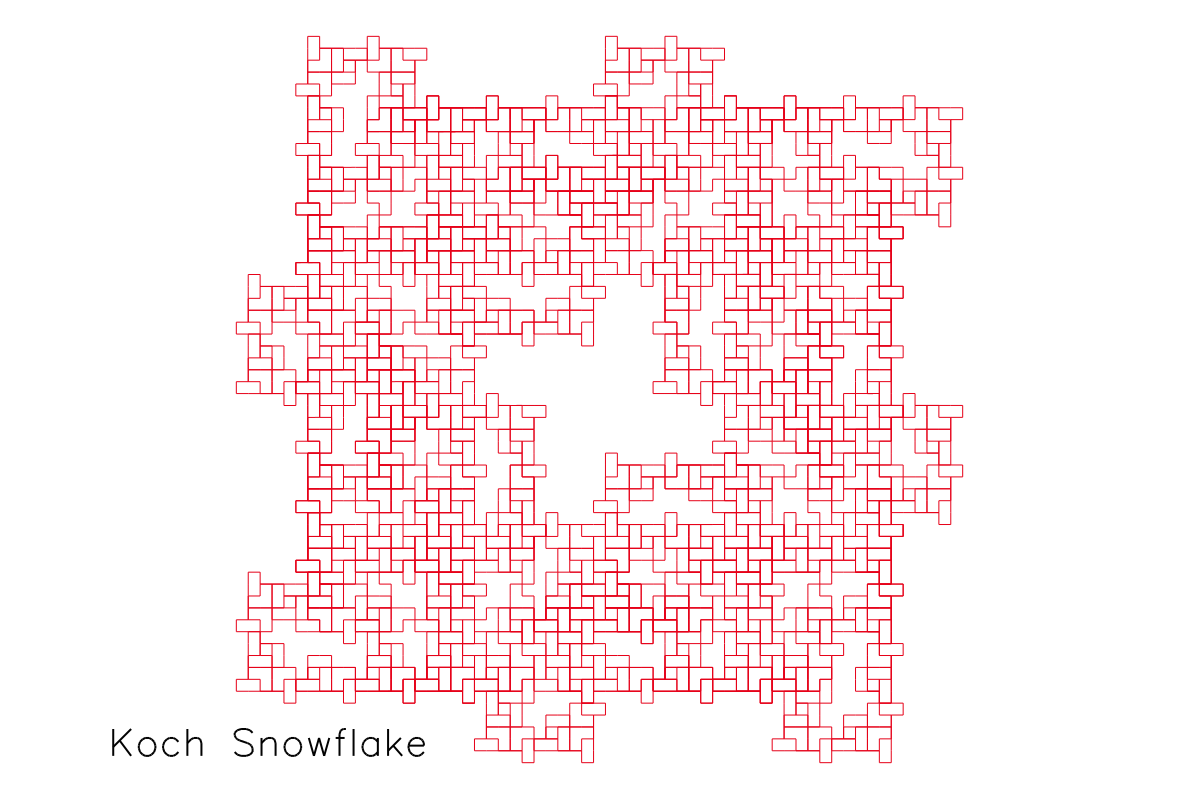
\includegraphics[width=\maxwidth]{../../temp/lsks001.eps}
  \caption{A Koch Snowflake (4 iterations)}
  \label{fig:lsks001}
\end{figure}

\begin{lstlisting}
RESET

STRING 1 F+F+F+F
STRING 2 F:FF+F-F+F+FF

STO 3 0

CSG GENERAL
COL 0.9 0 0.1

LSYSTEM 1 $1 90
\end{lstlisting}

\newpara
Finally, Figure~\ref{fig:lsgo001} shows a Gosper curve or ``flowsnake''
after 4 iterations, drawn by this script.

\begin{figure}
  \centering
  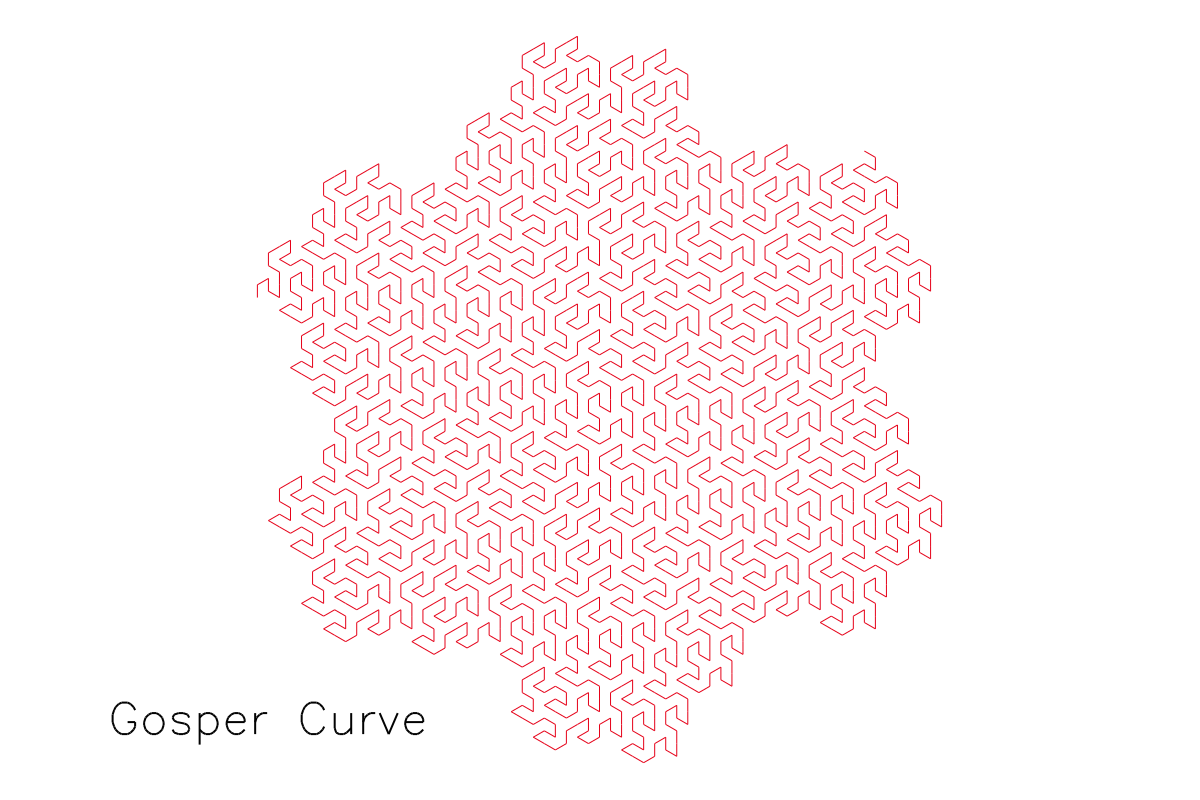
\includegraphics[width=\maxwidth]{../../temp/lsgo001.eps}
  \caption{A Gosper Flowsnake curve (4 iterations)}
  \label{fig:lsgo001}
\end{figure}

\begin{lstlisting}
RESET

STRING 1 F
STRING 2 F:F-D--D+F++FF+D-
STRING 3 D:+F-DD--D-F++F+D

STO 3 90

CSG GENERAL
COL 0.9 0 0.1

LSYSTEM 2 $1 60
\end{lstlisting}

\section{Fonts}
\newpara
As previously noted, the fonts that can be used in \textbf{GPLOT} are taken
from the Hershey vector fonts (originally published in 1967).
Figure~\ref{fig:fosm001} is a ``font sampler'' giving a quick overview
of what is available.

\begin{figure}
  \centering
  
\includegraphics[width=\maxwidth]{../../temp/fosm001.eps}
  \caption{A font sampler}
  \label{fig:fosm001}
\end{figure}

The pages that follow give full font tables for the
alphabetic, symbol and marker fonts. These can be used to
find the character numbers needed to insert special characters
in text, as well as showing all the fonts in detail.

\subsection{Alphabetic fonts}
This script will draw an alphabetic font table.
\begin{lstlisting}
PROC 1 I,10,I0IJ,M,I,TC   ; DRAW CHARACTER I AT IJ
PROC 2 I,0.5,-,1,STO,0.5,CHS,M,1,RCL,9.5,D
PROC 3 0.5,CHS,I,0.5,-,1,STO,M,9.5,1,RCL,D
PROC 4 I,10,I0IJ,0.4,-,SWAP,0.4,-,SWAP,M,I,1,TVI
STRING 1 "(I2)"
FONT 1 $1 
CANVAS -1 10 -1 10
CSG ALL
COLOUR 0 0 0
WIDTH 1
SYMHT 0.3 
ITEVAL 1 96 1 @1
FONT 1 SANS.SIMPLEX 
SYMHT 0.2 
COLOUR 0.5 0.5 0.5
ITEVAL 1 96 1 @4
COLOUR 1 0 0
ITEVAL 0 10 1 @2
ITEVAL 0 10 1 @3
MOVE 4.5 9.75
SYMHT 0.4
CTEXT 0 $1
\end{lstlisting}
The argument to this script is the font name.

\clearpage
\begin{figure}
  \centering
  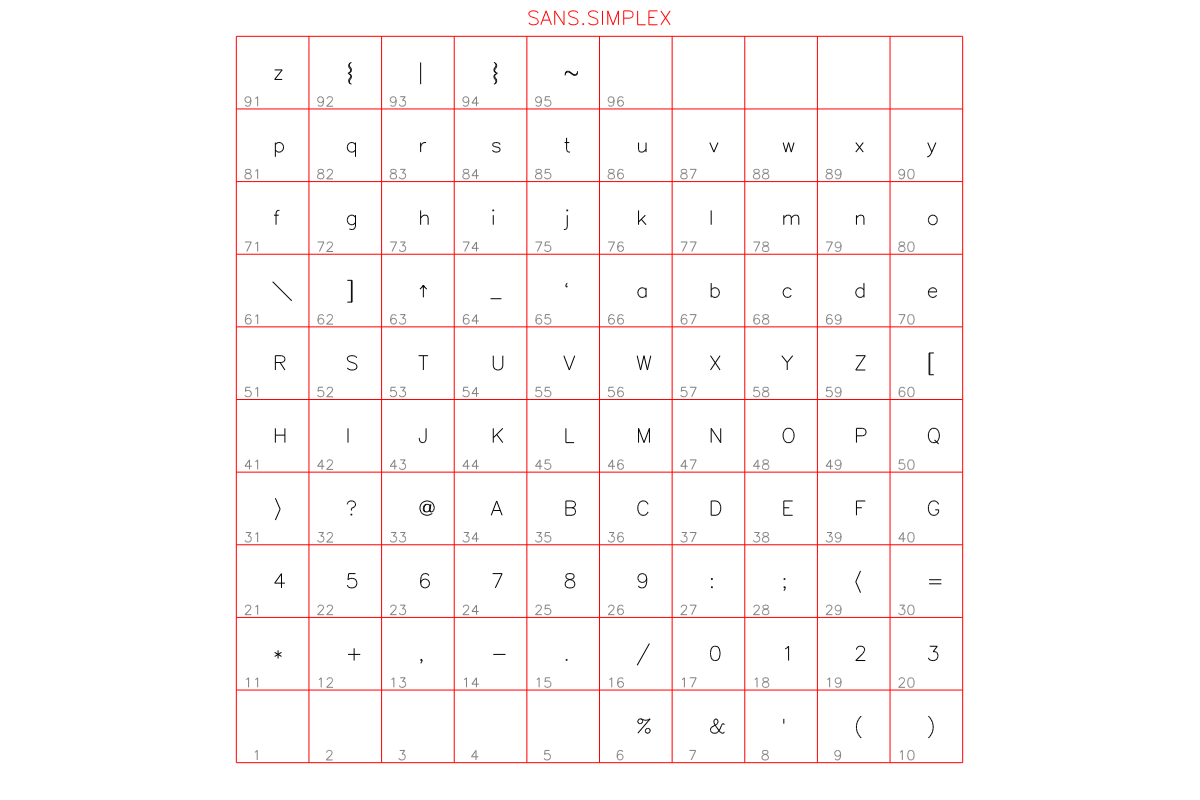
\includegraphics[width=\maxwidth]{../../temp/f01t001.eps}
  \caption{Sans Simplex}
  \label{fig:f01t001}
\end{figure}

\begin{figure}
  \centering
  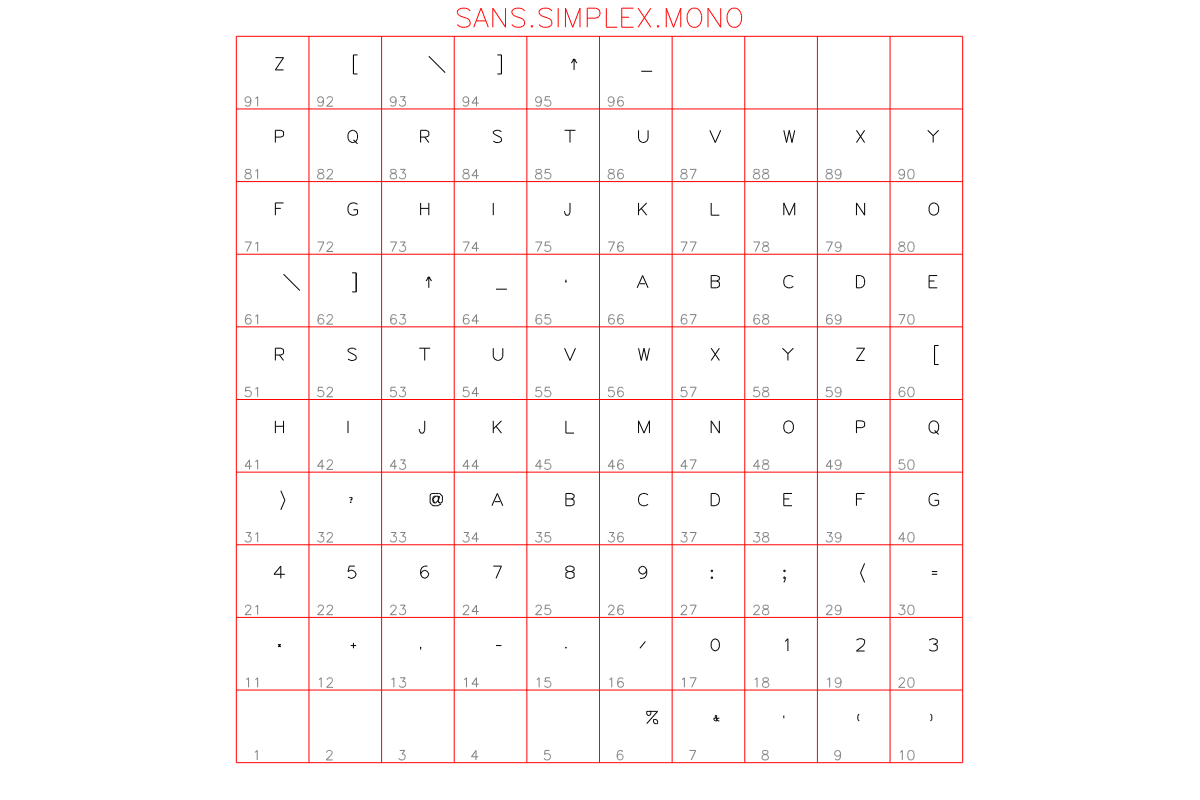
\includegraphics[width=\maxwidth]{../../temp/f02t001.eps}
  \caption{Sans Simplex Mono}
  \label{fig:f02t001}
\end{figure}

\clearpage
\begin{figure}
  \centering
  \includegraphics[width=\maxwidth]{../../temp/f03t001.eps}
  \caption{Sans Simplex Greek}
  \label{fig:f03t001}
\end{figure}

\begin{figure}
  \centering
  \includegraphics[width=\maxwidth]{../../temp/f04t001.eps}
  \caption{Sans Duplex}
  \label{fig:f04t001}
\end{figure}

\clearpage
\begin{figure}
  \centering
  \includegraphics[width=\maxwidth]{../../temp/f05t001.eps}
  \caption{Serif Complex}
  \label{fig:f05t001}
\end{figure}

\begin{figure}
  \centering
  \includegraphics[width=\maxwidth]{../../temp/f06t001.eps}
  \caption{Serif Complex Small}
  \label{fig:f06t001}
\end{figure}

\clearpage
\begin{figure}
  \centering
  \includegraphics[width=\maxwidth]{../../temp/f07t001.eps}
  \caption{Serif Complex Greek}
  \label{fig:f07t001}
\end{figure}

\begin{figure}
  \centering
  \includegraphics[width=\maxwidth]{../../temp/f08t001.eps}
  \caption{Serif Complex Greek Small}
  \label{fig:f08t001}
\end{figure}

\clearpage
\begin{figure}
  \centering
  \includegraphics[width=\maxwidth]{../../temp/f09t001.eps}
  \caption{Serif Triplex}
  \label{fig:f09t001}
\end{figure}

\begin{figure}
  \centering
  \includegraphics[width=\maxwidth]{../../temp/f10t001.eps}
  \caption{Serif Complex Italic}
  \label{fig:f10t001}
\end{figure}

\clearpage
\begin{figure}
  \centering
  \includegraphics[width=\maxwidth]{../../temp/f11t001.eps}
  \caption{Serif Complex Italic Small}
  \label{fig:f11t001}
\end{figure}

\begin{figure}
  \centering
  \includegraphics[width=\maxwidth]{../../temp/f12t001.eps}
  \caption{Serif Triplex Italic}
  \label{fig:f12t001}
\end{figure}

\clearpage
\begin{figure}
  \centering
  \includegraphics[width=\maxwidth]{../../temp/f13t001.eps}
  \caption{Script Simplex}
  \label{fig:f13t001}
\end{figure}

\begin{figure}
  \centering
  \includegraphics[width=\maxwidth]{../../temp/f14t001.eps}
  \caption{Script Complex}
  \label{fig:f14t001}
\end{figure}

\clearpage
\begin{figure}
  \centering
  \includegraphics[width=\maxwidth]{../../temp/f15t001.eps}
  \caption{Gothic Triplex}
  \label{fig:f15t001}
\end{figure}

\begin{figure}
  \centering
  \includegraphics[width=\maxwidth]{../../temp/f16t001.eps}
  \caption{Gothic Triplex German}
  \label{fig:f16t001}
\end{figure}

\clearpage
\begin{figure}
  \centering
  \includegraphics[width=\maxwidth]{../../temp/f17t001.eps}
  \caption{Gothic Triplex Italian}
  \label{fig:f17t001}
\end{figure}

\begin{figure}
  \centering
  \includegraphics[width=\maxwidth]{../../temp/f18t001.eps}
  \caption{Cyrillic Complex}
  \label{fig:f18t001}
\end{figure}


\clearpage
\subsection{Symbol fonts}

\newpara
This script draws a symbol font table:
\begin{lstlisting}
PROC 1 I,10,I0IJ,M,I,TS   ; DRAW SYMBOL I AT IJ
PROC 2 I,0.5,-,1,STO,0.5,CHS,M,1,RCL,9.5,D
PROC 3 0.5,CHS,I,0.5,-,1,STO,M,9.5,1,RCL,D
PROC 4 I,10,I0IJ,0.4,-,SWAP,0.4,-,SWAP,M,I,1,TVI
STRING 1 "(I2)"
FONT S $1 
CANVAS -1 10 -1 10
CSG ALL
COLOUR 0 0 0
WIDTH 1
SYMHT 0.3 
ITEVAL 1 96 1 @1
FONT 1 SANS.SIMPLEX 
SYMHT 0.2 
COLOUR 0.5 0.5 0.5
ITEVAL 1 96 1 @4
COLOUR 1 0 0
ITEVAL 0 10 1 @2
ITEVAL 0 10 1 @3
MOVE 4.5 9.75
SYMHT 0.4
CTEXT 0 $1
\end{lstlisting}
The argument is the font name.

\begin{figure}
  \centering
  \includegraphics[width=\maxwidth]{../../temp/f01s001.eps}
  \caption{Math symbols}
  \label{fig:f01s001}
\end{figure}

\begin{figure}
  \centering
  \includegraphics[width=\maxwidth]{../../temp/f02s001.eps}
  \caption{Cartographic symbols}
  \label{fig:f02s001}
\end{figure}

\clearpage
\begin{figure}
  \centering
  \includegraphics[width=\maxwidth]{../../temp/f03s001.eps}
  \caption{Astronomical symbols}
  \label{fig:f03s001}
\end{figure}

\begin{figure}
  \centering
  \includegraphics[width=\maxwidth]{../../temp/f04s001.eps}
  \caption{Astrological symbols}
  \label{fig:f04s001}
\end{figure}

\clearpage
\begin{figure}
  \centering
  \includegraphics[width=\maxwidth]{../../temp/f05s001.eps}
  \caption{Musical symbols}
  \label{fig:f05s001}
\end{figure}

%% \clearpage
\subsection{Marker font}

\newpara
This script draws a marker font table:
\begin{lstlisting}
PROC 1 I,10,I0IJ,M,I,TM   ; DRAW MARKER I AT IJ
PROC 2 I,0.5,-,1,STO,0.5,CHS,M,1,RCL,9.5,D
PROC 3 0.5,CHS,I,0.5,-,1,STO,M,9.5,1,RCL,D
PROC 4 I,10,I0IJ,0.4,-,SWAP,0.4,-,SWAP,M,I,1,TVI
STRING 1 "(I2)"
FONT M $1 
CANVAS -1 10 -1 10
CSG ALL
COLOUR 0 0 0
WIDTH 1
SYMHT 0.3 
ITEVAL 1 96 1 @1
FONT 1 SANS.SIMPLEX 
SYMHT 0.2 
COLOUR 0.5 0.5 0.5
ITEVAL 1 96 1 @4
COLOUR 1 0 0
ITEVAL 0 10 1 @2
ITEVAL 0 10 1 @3
MOVE 4.5 9.75
SYMHT 0.4
CTEXT 0 $1
\end{lstlisting}
The argument is the font name.

\begin{figure}
  \centering
  \includegraphics[width=\maxwidth]{../../temp/f01m001.eps}
  \caption{Principal marker font}
  \label{fig:f01m001}
\end{figure}


\section{Acknowledgements and history}
\newpara
\textbf{GPLOT} is entirely reliant on \textbf{DIMFILM}, written by Dr. John C. Gilbert at The University of London
Computer Centre (U.L.C.C.) and maintained primarily by him between 1972 and the mid-1990's. One goal of \textbf{GPLOT} is to
preserve \textbf{DIMFILM}. I can find almost no trace of this excellent software elsewhere.

\newpara
\textbf{GPLOT} uses character
string parsing subroutines written by Dr. Adrian Clark circa 1985. Dr. Clark also wrote a \textbf{DIMFILM} device
driver for Tektronix storage tube terminals on which the \textbf{GPLOT} Tektronix support
is based.

\newpara
The version of \textbf{DIMFILM} used here came to me from Dr. Gilbert via Dr. Clark in 2005. Due to a malfunctioning hardware
RAID controller, the U.L.C.C. production version was no longer available and the version we have here
was assembled by Dr. Gilbert from various sources. Unfortunately, it did not include the original font data. I had a
working version of \textbf{DIMFILM} using Hershey fonts by 2007 (it was very much a hobby project!). Not many changes were made.
The original, unmodified, source is retained in the \texttt{historic} sub-tree of the source repository.

\newpara
The original (albeit ``interim'') \textbf{DIMFILM} manual was preserved in several formats, including a very early version
of Microsoft Word and some mid-1980's version of WordStar. I have failed to find any software which can use these
files. Fortunately, the manual was also kept in a RUNOFF style format (i.e. plain text with markup). I never found
a RUNOFF style formatting program that could process these files either (the files have the extension \texttt{.sg} which
doesn't seem to be known to the Internet for text processing purposes). However, it was possible to write a
formatter in Python from scratch to get a PDF version of this essential manual.

\newpara
The first usable version of \textbf{GPLOT} (0.1, late 2013) 
could not output EPSF files as such, but used a
limited character set format that could be trivially translated to EPSF. V0.2 (2022) improved Tektronix 401x support. V0.58
(developed between late 2022 and early 2023) added significant -- if idiosyncratic -- facilities for function evaluation 
and other programmability features, as well as SVG output. It also exposed a lot more of \textbf{DIMFILM's} capabilities and directly
generated "true" EPS files. Most of what can be done with \textbf{DIMFILM} using a specially
written Fortran program can now be done from \textbf{GPLOT}. V0.59 fixed some bugs in parameter substitution. V0.6 (July 2025)
tidied up a few things and supported building on ``Unix-like'' systems as well as NOS. This version also uses the NOS MODIFY --
Git inter-operability tools so that the source can be managed equally well on NOS or with Git, with changes made on one system
being automatically reflected in the other. This version also automatically generates minor variations of the source code
needed for building on COS and Unix, using a single, NOS compatible, code base. Many further changes and additions were made
between July and October 2025 -- many of them a direct result of trying to use it (e.g. to produce the figures
in this manual). The additions include the ``higher level drawing'' functions.

\newpara
The current version (0.87) may be genuinely useful (I find it to be). 

\clearpage
\begin{figure}
  \centering
  \includegraphics[angle=90,scale=1.5]{../../temp/cht1001.eps}
\end{figure}


\clearpage
\begin{figure}
  \centering
  \includegraphics[angle=90,scale=1.5]{../../temp/cht2001.eps}
  \label{fig:cht2001}
\end{figure}


\clearpage
\begin{figure}
  \centering
  \includegraphics[width=\maxwidth]{../../temp/fin001.eps}
  \caption{THE END}
  \label{fig:fin001}
\end{figure}


\end{document}

